\documentclass[twosideprint]{politex}
% ========== Opções ==========
% pnumromarab - Numeração de páginas usando algarismos romanos na parte pré-textual e arábicos na parte textual
% abnttoc - Forçar paginação no sumário conforme ABNT (inclui "p." na frente das páginas)
% normalnum - Numeração contínua de figuras e tabelas 
%	(caso contrário, a numeração é reiniciada a cada capítulo)
% draftprint - Ajusta as margens para impressão de rascunhos
%	(reduz a margem interna)
% twosideprint - Ajusta as margens para impressão frente e verso
% capsec - Forçar letras maiúsculas no título das seções
% espacosimples - Documento usando espaçamento simples
% espacoduplo - Documento usando espaçamento duplo
%	(o padrão é usar espaçamento 1.5)
% times - Tenta usar a fonte Times New Roman para o corpo do texto
% noindentfirst - Não indenta o primeiro parágrafo dos capítulos/seções


% ========== Packages ==========
\usepackage[utf8]{inputenc}
\usepackage{amsmath,amsthm,amsfonts,amssymb}
\usepackage{graphicx,cite,enumerate}
\usepackage{listings}
\usepackage[brazil]{babel}
%\usepackage[english]{babel}
%\usepackage{caption}
%\usepackage{subcaption}
% ========== ABNT (requer ABNTeX 2) ==========
%	http://www.ctan.org/tex-archive/macros/latex/contrib/abntex2
\usepackage[num,overcite]{abntex2cite}

% Forçar o abntex2 a usar [ ] nas referências ao invés de ( )
\citebrackets{[}{]}

% ========== Lorem ipsum ==========
\usepackage{blindtext}

\usepackage{array}

\newcommand{\legend}[1]{\begin{center}\def\caption{}\caption{#1}\end{center}}
% \newcommand{\legend}[1]{\begin{center}\def\caption{}\makebox[\textwidth][s]{\caption{#1}} \par\end{center}}

% ========== Opções do documento ==========
% Título
\titulo{Formicarium: Ambiente de desenvolvimento em tempo real para microsserviços}

% Autor
\autor{Leonardo C. S. Iacovini\\
		Luiz G. Santos\\
		Rafael L. D. R. Santos\\
		Rafael R. Correia}

% Orientador / Coorientador
\orientador{Jorge Risco Becerra}
\coorientador{Rafael de França Ferreira}

% Tipo de documento
\tcc{de Computação}
%\dissertacao{Engenharia Elétrica}
%\teseDOC{Engenharia Elétrica}
%\teseLD
%\memorialLD

% Departamento e área de concentração
\departamento{PCS}
\areaConcentracao{Engenharia de Software}

% Local
\local{São Paulo}

% Ano
\data{2018}




\begin{document}
% ========== Capa e folhas de rosto ==========
\capa
% \falsafolhaderosto
\folhaderosto


% ========== Folha de assinaturas (opcional) ==========
%\begin{folhadeaprovacao}
%	\assinatura{Prof.\ X}
%	\assinatura{Prof.\ Y}
%	\assinatura{Prof.\ Z}
%\end{folhadeaprovacao}


% ========== Ficha catalográfica ==========
% Fazer solicitação no site:
%	http://www.poli.usp.br/en/bibliotecas/servicos/catalogacao-na-publicacao.html


% ========== Dedicatória (opcional) ==========
%\dedicatoria{Dedicatória}


% ========== Agradecimentos ==========
\begin{agradecimentos}
Risco
Ferreira
Nubank

\end{agradecimentos}


% ========== Epígrafe (opcional) ==========
\epigrafe{
	\emph{``The ability to simplify means to eliminate the unnecessary so that the necessary may speak.''}
	\begin{flushright}
		-{}- Hans Hofmann
\end{flushright}
}


% ========== Resumo ==========
\begin{resumo}
	Em uma arquitetura distribuída de microsserviços, é comum enfrentar problemas relacionados à produtividade enquanto o software é desenvolvido. Uma das causas deste problema é a necessidade de se executar diversos microsserviços ao mesmo tempo para iterar, testar e validar algum fluxo de negócio. Estes processos computacionais demandam uma quantidade de recursos (processamento e memória) que nem sempre estão disponíveis na máquina do desenvolvedor.
	
	Um outro problema comum é a dificuldade de se entender e depurar fluxos complexos de negócio que envolvam comunicação entre diversos microsserviços através de diferentes protocolos de troca de mensagens.
	
	Foi neste contexto que surgiu a parceria entre a Poli e o Nubank para o desenvolvimento de um projeto que tentasse mitigar os problemas acima descritos.
	
%%	O Nubank é uma fintech brasileira que conta com mais de 200 engenheiros, trabalhando diariamente em mais de 200 microsserviços para atender os mais de 5 milhões de clientes ativos em seus diversos produtos. A empresa é referência nacional e mundial em tecnologia, devido a sua arquitetura de software moderna, baseada em microsserviços. Porém, as implicações negativas deste modelo já estão se manifestando na empresa há algum tempo, prejudicando a produtividade das equipes.
	
	O projeto foi co-orientado por um dos engenheiros mais prestigiados do Nubank, que está presente na empresa desde praticamente o seu nascimento, sendo responsável por importantes decisões arquiteturais e por ter participado da construção da fundação de toda a tecnologia da empresa.
	
	Através do intenso uso de computação em nuvem, orquestração de Containers Docker, conceitos de Distributed Tracing e técnicas para sincronização de file systems, este projeto visa aumentar a produtividade dos engenheiros do Nubank em suas tarefas de desenvolvimento e manutenção dos microsserviços da empresa.
	
	Para o desenho da solução, foi feito um estudo profundo sobre modelos de PaaS, características de microsserviços de modo geral, bem como seu uso no contexto específico do Nubank. 
	
	O resultado foi a construção de um ambiente de desenvolvimento para arquiteturas de larga escala baseada em microsserviços, chamado de Formicarium. O projeto foi implantado em um squad do Nubank nos últimos meses de desenvolvimento do trabalho para que feedbacks pudessem ser colhidos e para que fossem feitos os ajustes necessários.
	
	Com base nos resultados, pode-se concluir que o projeto conseguiu atender os requisitos propostos e mitigar os diversos problemas apresentados. A sua implantação foi bem recebida pelo squad escolhido e sua difusão não é uma tarefa complicada, dado sua fácil utilização e vantagens imediatas. Inclusive, ao longo do projeto foi tomado o cuidado de se extrair os componentes altamente acoplados com características específicas do Nubank, de modo que a implantação da solução até mesmo em outras empresas fosse possível sem muitas modificações.
	
%
% \\[3\baselineskip]
%
\textbf{Palavras-Chave} -- Microsserviço, Docker, Kubernetes, Computação em Nuvem, Distributed Tracing.
\end{resumo}


% ========== Abstract ==========
\begin{abstract}
Abstract...
%
\\[3\baselineskip]
%
\textbf{Keywords} -- Word, Word, Word, Word, Word.
\end{abstract}


% ========== Listas (opcional) ==========
\listadefiguras
\listadetabelas

% ========== Listas definidas pelo usuário (opcional) ==========
%\begin{pretextualsection}{Lista de símbolos}

%Lista de símbolos...

%\end{pretextualsection}

% ========== Sumário ==========
\sumario



% ========== Elementos textuais ==========

%\part{Introdução}
\chapter{Introdução}
	\section{Objetivo}
	%% O que o seu projeto resolve?
	O objetivo deste trabalho é criar um ambiente e um ferramental para acelerar a iterações no desenvolvimento de microsserviços em uma arquitetura de larga escala.
	\section{Motivação}
	%% Por que fazer um trabalho?
	A motivação desse projeto vem de alguns fatores. O primeiro é o interesse e a familiaridade do grupo quanto ao desenvolvimento de microsserviços provenientes da experiência adquirida nos estágios na Nubank, e o reconhecimento dos benefícios e dificuldades essa arquitetura. Outro fator importante é a constatação de que, com o crescimento das aplicações em nuvem computacional, a necessidade e urgência de uma arquitetura distribuída aumenta, e a carência de ferramentas para conter suas dificuldades se torna um problema cada vez mais importante.
	
	Com isso, foi possível a identificação de um problema relativamente complexo de Engenharia de Software que ainda não teve a devida atenção no mercado, e uma oportunidade para aplicação e aprofundamento do nosso conhecimento de processo de desenvolvimento de software. Nós queríamos, então, criar uma proposta de solução para um problema real ainda em discussão.
	\section{Justificativa}
	%% Por que fazer esse trabalho? 
	%% 1. O tema é necessário (debugging microservices)
	O crescimento da arquitetura de microsserviços é notório e pode ser percebido de várias formas. Tanto no mercado quanto na academia, a discussão só tem crescido, com cada vez mais empresas grandes decidindo adotar essa tecnologia, tais como Uber e Netflix. É possível notar também um crescente número de livros que tratam sobre o assunto, como \textit{Production-Ready Microservices} da Susan J. Fowler\cite{productionreadyms} e \textit{Microservices Patterns} de Chris Richardson\cite{mspatterns}. Esse crescimento permitiu a escalabilidade dessas empresas, mas também veio com um custo: a crescente complexidade.
	
	É nesse contexto que o Nubank se encontra e faz parceria neste trabalho. O Nubank é uma fintech brasileira que conta com cerca de 200 engenheiros, trabalhando diariamente em mais de 200 microsserviços para atender os mais de 5 milhões de clientes ativos em seus diversos produtos. A empresa é referência nacional e mundial em tecnologia, devido a sua arquitetura de software moderna, baseada em microsserviços. Porém, as implicações negativas deste modelo já estão se manifestando na empresa há algum tempo, prejudicando a produtividade das equipes. Assim, tivemos a oportunidade de firmar essa parceria e trabalharmos em um contexto real, para resolver uma carência crescente na empresa.
	
	No entanto, este trabalho foi feito de tal forma que, com algum esforço de implantação, as ferramentas desenvolvidas possam ser usufruídas por outras empresas que tenham características de arquitetura semelhantes. Um estudo feito na Universidade de Brighton, no Reino Unido, indica que dentre 33 publicações referentes à arquitetura de microsserviços, o desafio mais citado é referente a comunicação e integração dos microsserviços.\cite{systematicmapping}
	%% 4. Há evidência de que outros contextos podem se beneficiar desse projeto.
	%%\cite{fowlermicroservices}
	\section{Organização do Trabalho}
	%% Como ler esse texto?
	
\chapter{Aspectos Conceituais}
    
    \section{Ambiente de desenvolvimento}
    
    O ambiente de desenvolvimento de um projeto de desenvolvimento de software é o termo usado para todos os itens de que o projeto precisa para desenvolver e implantar o sistema, como, por exemplo, ferramentas, diretrizes, processo, \textit{templates} e infra-estrutura.\cite{ambientedev}
    
    Geralmente temos alguns ambientes de de software bem comuns como Produção, Homologação e Desenvolvimento. Cada um desses ambientes possui suas características próprias e requisitos de funcionamento e ferramental.
    
    Em especial o ambiente de desenvolvimento incluem as ferramentas utilizadas pelo desenvolvedor para escrever, executar e testar sua aplicação, nesse contexto temos editores de texto, ferramentas de linha de comando, executores de teste, plataformas de contêineres locais para execução de serviços, entre outros.
    
    \section{Desenvolvimento em tempo real} %% TODO
    
    Quando falamos de "tempo real" esperamos que o tempo entre ação e \textit{feedback} seja curto o suficiente para atender os requisitos de uma determinada aplicação. No caso de desenvolvimento em tempo real, queremos que o tempo de iteração no processo de escrita de código e validação deste, seja curto o suficiente para não prejudicar o fluxo de desenvolvimento do desenvolvedor, geralmente estamos falando de algo na casa de segundos até poucos minutos.
    
    Esse tempo pode ser por exemplo, o intervalo de tempo levado para execução de testes unitários ou de integração que são usados pelo desenvolvedor. Aqui não se incluem processos que são executados em pipelines automatizadas ou sistemas de CI/CD, somente as ferramentas utilizadas pelo desenvolvedor no dia a dia.
    
    \section{Contêineres} %% TODO: Paps 
	    \subsection{Breve história da tecnologia}
	    A história dos Contêineres começa em 1979 no Unix L7. Nele foi introduzido a chamada de sistema (\textit{system call}) \textit{chroot} capaz de mudar o diretório raiz de um processo e de seus processos filhos para um novo local no sistema de arquivos. Este avanço foi o início do conceito de isolamento de processos, pois limitava o acesso de cada processo ao sistema de arquivos. 

	    Em 2000, surgiu o FreeBSD Jail, que permitia a administradores particionar um sistema FreeBSD em vários sistemas menores isolados e independentes, chamados de “\textit{jails}”. O sistema é similar ao \textit{chroot}, mas incluiu recursos de isolamento adicionais em diversos aspectos do sistema operacional, como por exemplo a atribuição de um endereço de IP diferente para cada \textit{jail}. \cite{abriefhistoryofcontainers}

	    Em 2001, foi lançado o Linux VServer que, assim como o FreeBSD Jail, também é um mecanismo de \textit{jail} que pode particionar recursos (sistema de arquivos, endereços de rede, memória) em um sistema computacional. Isso é realizado por meio de níveis de isolamento do \textit{kernel}. Cada partição é chamada \textit{security context} e o sistema virtualizado dentro dele é chamado de \textit{virtual private server}. \cite{linuxvserver}

    	Em 2004, foi lançado o Solaris Zones para sistemas x86 e SPARC. Cada \textit{zone} age como um servidor virtual completamente isolado dentro de uma única instância. Existem dois tipos de \textit{zones}: zonas globais (\textit{Global Zones}) e não-globais (\textit{Non-Global Zones}). A zona global é o ambiente de SO tradicional e é a área onde o SO Solaris está instalado. Todas as operações do sistema, como instalações, inicializações e desligamentos são feitas na zona global. As zonas não-globais, comumente chamadas somente de zonas, tem seus recurso e limites definidos pela zona global a que pertencem  \cite{introductiontosolariszone}

    	Em 2005 a empresa Virtuozzo lançou o OpenVZ, que utiliza o \textit{kernel} do Linux para fornecer virtualização, isolamento, gerenciamento de recursos e \textit{checkpointing}. Cada contêiner OpenVZ possui um sistema de arquivos isolado, usuários e grupos de usuários, uma árvore de processos, rede, dispositivos e comunicação entre processos. Uma desvantagem da solução é que seu funcionamento depende da aplicação de um \textit{patch} no \textit{kernel} do Linux. \cite{openvz}

    	Em 2006 engenheiros da Google desenvolveram o Process Containers, projetado para limitar, contabilizar e isolar o uso de recursos computacionais (CPU, memória, I/O do disco, rede) de uma coleção de processos. Um ano depois o projeto foi renomeado para Control Groups (\textit{cgroups}) e foi adicionado ao \textit{kernel} do Linux na versão \textit{2.6.24}.

    	Em 2008 surgiu o LXC (LinuX Containers), que foi a primeira e mais completa implementação de um gerenciador de contêineres Linux. Foi implementado utilizando \textit{cgroups} e Linux \textit{namespaces} e funciona no \textit{kernel} do Linux sem a necessidade da aplicação de \textit{patches}.
	
    	Em 2011 a empresa CloudFoundry iniciou o projeto Warden, que utilizava LXC em suas primeiras implementações, porém depois foi substituído por soluções próprias da empresa. Warden roda em formato \textit{daemon} e pode isolar ambientes em qualquer sistema operacional. Além disso, provê uma API para o gerenciamento de \textit{cgroups}, \textit{namespaces}, ciclo de vida dos processos e dos contêineres em diversos \textit{hosts} através de um modelo cliente-servidor.

    	Finalmente, em 2013, surgiu o Docker. Neste momento contêineres cresceram muito em popularidade, juntamente com o Docker em si.
	    Assim como o Warden, o Docker utilizou LXC em seus primeiros estágios mas logo trocou por uma solução própria para gerenciamento de     contêineres: o \textit{libcontainer}.
	    O Docker se destacou de seus concorrentes por oferecer um ecossistema completo para o gerenciamento de contêineres, que será detalhado mais adiante.
	
	\subsection{Diferenças com Máquinas virtuais}
	
	A virtualização é a tecnologia que permite a criação de diferentes ambientes computacionais, chamados de virtuais por simular a interface que é esperada por um sistema operacional.
	
	Um dos principais componentes da arquitetura é o \textit{Hypervisor}. Ele gerencia a distribuição dos recursos computacionais na máquina física (armazenamento, processamento e memória) entre as várias máquinas virtuais, além de fornecer um isolamento entre elas. Ele é um componente que fica entre o \textit{hardware} e a máquina virtual e é necessário para o processo de virtualização.
	Entre os gerenciadores de máquinas virtuais mais populares no mercado, pode-se citar VMWare vSphere, VirtualBox, Xen, Hyper-V e KVM.

	No baixo nível, um contêiner é apenas um conjunto de processos que são isolados do resto do sistema. No caso do Docker, os contêineres compartilham o \textit{kernel} do sistema operacional hospedeiro e, frequentemente, os binários e bibliotecas também. Todos os componentes compartilhados são \textit{read-only}. Este compartilhamento de componentes reduzem a necessidade de se replicar código do sistema operacional, e isso significa que um único servidor pode executar múltiplos contêineres com uma única instalação do sistema operacional.

	Diferentemente, uma máquina virtual é constituída do espaço de usuário juntamente com o espaço do \textit{kernel} de um sistema operacional e o \textit{hardware} é virtualizado. Cada máquina virtual tem um sistema operacional e suas aplicações e elas compartilham entre si o \textit{hardware} do computador hospedeiro.

	Ambas as tecnologias provém ambientes isolados para execução de aplicações e podem ser utilizadas para empacotar e distribuir \textit{software}.

	Dado o menor número de camadas entre a aplicação e o \textit{hardware},  os contêineres tendem a ser mais leves e mais rápidos, tornando-os mais práticos para os ciclos de desenvolvimento e implantação de serviços. Comparativamente, o tempo de inicialização de uma máquina virtual é muito maior do que a de um contêiner equivalente, além de o espaço ocupado em disco ser uma ordem de magnitude maior. \cite{whatsthediffvmvscontainers}
	
	\begin{figure}[htb]
		\caption{\label{fig_circulo}Diferenças entre VMs e Contêiners}
		\begin{center}
    		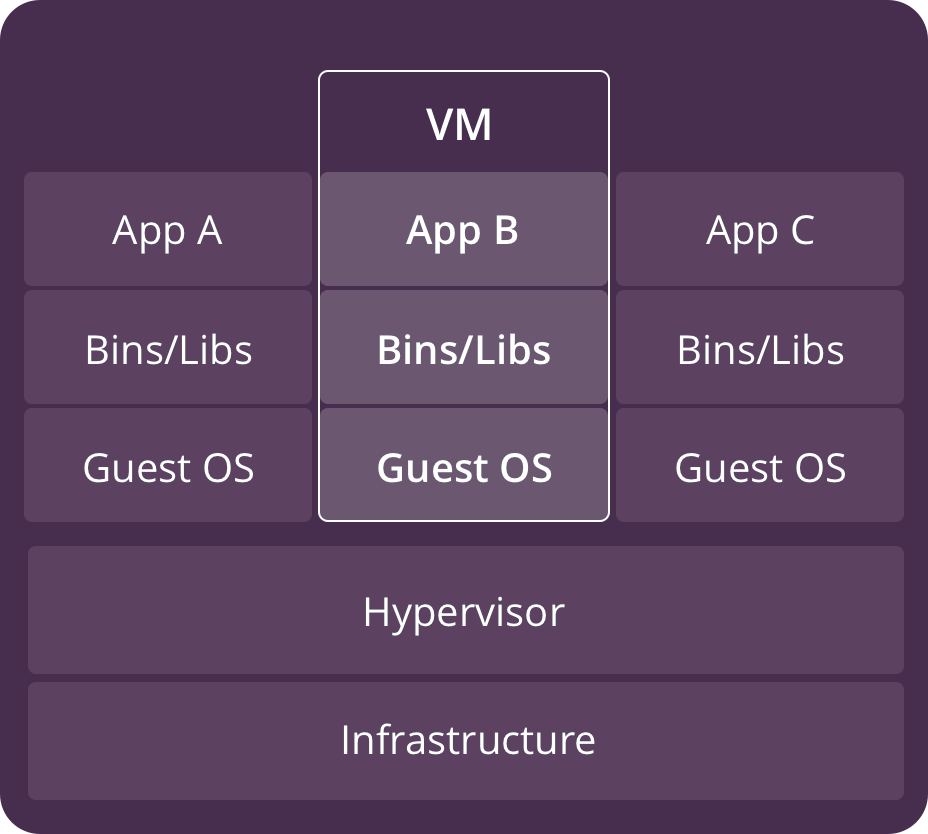
\includegraphics[scale=0.20]{pictures/vms.png}
    		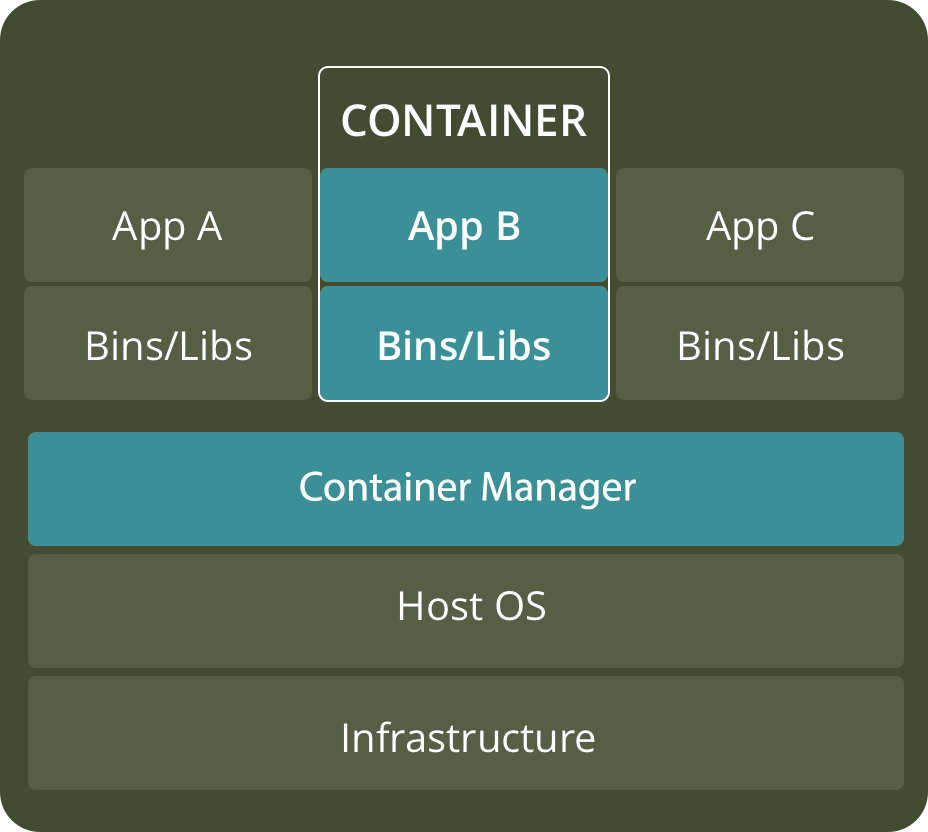
\includegraphics[scale=0.20]{pictures/containers.png}
		\end{center}
		\legend{Fonte: https://www.backblaze.com/blog/vm-vs-containers/}
	\end{figure}
	
	Ambos têm vantagens e desvantagens, e a decisão entre um outro varia dependendo dos casos de uso específicos, mas pode-se utilizar as seguintes regras como um ponto de partida:
	
	Máquinas virtuais são melhores para executar aplicações que necessitam de todos os recursos e funcionalidades do sistema operacional ou quando há uma variedade de sistemas operacionais para se gerenciar.
	
	Contêineres são uma escolha melhor quando a maior prioridade é maximizar o número de aplicações sendo executadas em um número mínimo de servidores.
	
	\section{Cloud Computing}
	Computação em Nuvem (do Inglês \textit{Cloud Computing}) é segundo a NIST \footnote{National Institute of Standards and Technology, https://www.nist.gov/} um modelo para prover um acesso de rede a um grupo compartilhado (\textit{shared pool}) de recursos computacionais (recursos como capacidade de rede, servidores, armazenamento, aplicações e serviços) de forma ubíqua, prática e sob demanda.

    Tal acesso deve ser rapidamente provisionado e lançado com o mínimo de gerenciamento e interação com o provedor de serviços por parte da aplicação.

    O modelo de computação em nuvem deve possuir algumas características básicas, que estão descritas na seção seguinte.

        \subsection{Características básicas de Cloud Computing}

            A NIST define 5 características essenciais do modelo de Cloud Computing:
            \begin{itemize}
            	\item Serviço sob demanda: Um consumidor pode provisionar unilateralmente capacidades computacionais, como tempo de servidor e armazenamento de rede, conforme for necessário, sem qualquer interação humana com o provedor de serviço;
            	
            	\item Agrupamento de recursos: Os recursos de computação do provedor são agrupados para atender a vários consumidores usando um modelo "multi inquilino", com diferentes recursos físicos e virtuais dinamicamente atribuídos e reatribuídos de acordo com a demanda do consumidor. Existe uma sensação de independência de localização pois o cliente geralmente não tem controle ou conhecimento sobre a localização exata dos recursos fornecidos, mas pode ser capaz de especificar a localização em um nível de abstração (por exemplo, país, estado ou datacenter). Exemplos de recursos incluem armazenamento, processamento, memória e largura de banda de rede.
            	
            	\item Amplo acesso à rede: Os recursos estão disponíveis na rede e são acessados por meio de mecanismos que promovam o uso por plataformas heterogêneas por clientes em diversos dispositivos (por exemplo, telefones celulares, tablets, laptops e estações de trabalho). Esta característica promove o conceito de computação ubíqua, isto é, em toda parte, onipresente.
            	
            	\item Elasticidade rápida: Os recursos podem ser provisionados e liberados elasticamente, em alguns casos automaticamente, proporcionando uma escalabilidade crescente ou descrescente conforme a demanda. Os recursos disponíveis normalmente aparentam ser ilimitados para o consumidor, podendo ser requisitidados em qualquer quantidade e a qualquer momento.
            	
            	\item Serviço mensurável: Os sistemas em nuvem controlam e otimizam automaticamente o uso de recursos, aproveitando-se de uma capacidade de medição em um nível de abstração apropriado ao tipo de serviço (por exemplo, armazenamento, processamento, largura de banda e contas de usuário ativas). O uso de recursos pode ser monitorado, controlado e reportado, gerando transparência tanto para o fornecedor e consumidor do serviço utilizado.
            \end{itemize}

        \subsection{Modelos para Cloud Computing}

        Este capítulo introduz brevemente os modelos de serviço de cloud computing que podem ser adotados por um provedor e os modelos de     \textit{deployment}, nas secções seguintes.

\subsection{Modelos de serviços}

A teoria por trás dos serviços de computação em nuvem abrange três elementos principais: software, plataforma e infraestrutura. Temos os seguintes modelos de serviço:

\begin{itemize}
  \item \textbf{SaaS, Software as a Service} ("Software como um serviço") 

  Neste modelo é oferecido ao consumidor o uso de aplicações de um provedor que rodam sobre uma infraestrutura em nuvem. Estas aplicações são acessíveis a partir de vários dispositivos clientes por meio de uma interface simples, como um navegador da web, ou uma interface de por meio de um programa (mobile ou desktop). 

  O consumidor não gerencia ou controla a infraestrutura de nuvem por trás da aplicação, incluindo rede, servidores, sistemas operacionais, armazenamento ou capacidade da aplicação individual. São disponibilizadas apenas configurações do aplicativo específicas para aquele usuário individual.

  Alguns exemplos de SaaS são serviços de \textit{webmail}, \textit{streaming} de vídeos, conversão de arquivos e trabalho colaborativo com arquivos. Este modelo não será mais detalhado neste trabalho.

  \item \textbf{PaaS, Platform as a Service} ("Plataforma como um serviço") 

  A capacidade fornecida ao consumidor é de implantar na nuvem aplicações criadas por meio de linguagens de programação, bibliotecas, serviços e ferramentas suportadas pelo provedor. Tais aplicações podem ser criadas pelo próprio consumidor, ou consumidas por este.

  Assim como no modelo de SaaS, o consumidor geralmente não gerencia ou têm controle sobre a infraestrutura de nuvem por trás, incluindo rede, servidores, sistemas operacionais, ou armazenamento. Porém o consumidor as tem controle sobre os aplicativos implantados e possivelmente sobre definições de configuração para o ambiente de hospedagem do aplicativo.

  Como exemplos de provedores no mercado temos \textit{IBM Bluemix}, \textit{Heroku}, e \textit{Windows Azure Cloud}.

  \item \textbf{IaaS, Infrastructure as a Service} ("Infraestrutura como um serviço") 

  A capacidade oferecida ao consumidor é provisionar processamento, armazenamento, redes e outros recursos fundamentais de computação onde o consumidor é capaz de implantar e executar software arbitrário, incluindo-se sistemas e aplicações. O consumidor não gerencia nem controla a infraestrutura de nuvem por trás, mas tem controle sobre sistemas operacionais, armazenamento e aplicativos implantados. Possivelmente possui também um controle limitado de componentes de rede (por exemplo, firewalls de host). Geralmente acompanha serviços de máquinas virtualizadas.

  Alguns exemplos de provedores no mercado são \textit{Amazon Web Services}, \textit{Microsoft Azure}, \textit{Google Cloud} e \textit{VMware Cloud on AWS}. 
\end{itemize}

	\section{Programação Funcional}
	
	Como o próprio nome diz, a programação funcional surge de funções matemáticas, mais especificamente do cálculo lambda. Programação funcional é um paradigma de programação assim como Orientado a Objeto ou Imperativo. As características mais marcantes desse paradigma são a presença de imutabilidade de dados e estados, funções serem tratadas como valores como quaisquer outros tipos (inteiros, strings, etc...), transparência referencial e separação de efeitos colaterais.
	As linguagens de programação podem ser puramente funcionais, ou parcialmente, isso é, contém elementos desse paradigma porém não se limitam a ele, ou fazem pequenos desvios em prol da usabilidade.
	
	\section{Microsserviços}
	
	Microsserviços é um termo usado para designar uma arquitetura de software distribuída que possui um certo conjunto de características, como por exemplo o deploy independente. É uma abordagem de desenvolvimento que que permite a criação de uma aplicação única através de um conjunto de pequenos serviços, de modo que cada um é responsável apenas por uma pequena parte do processo e durante sua execução eles se comunicam por meio de mecanismos leves, geralmente uma API e/ou mensageria (mas não se limitando a esses). Cada um dos serviços é focado em uma parte atômica da lógica de negócio e funcionam através de mecanismos de deploy independente e automatizado. Em contraste a esse tipo de arquitetura temos uma aplicação monolítica, que se caracteriza pela centralização da lógica e código em apenas um serviço de grande porte. \cite{microsservicos}
	
	\begin{figure}[htpb]
	    \caption{Microsserviços vs Monolitos}
	    \begin{center}
	        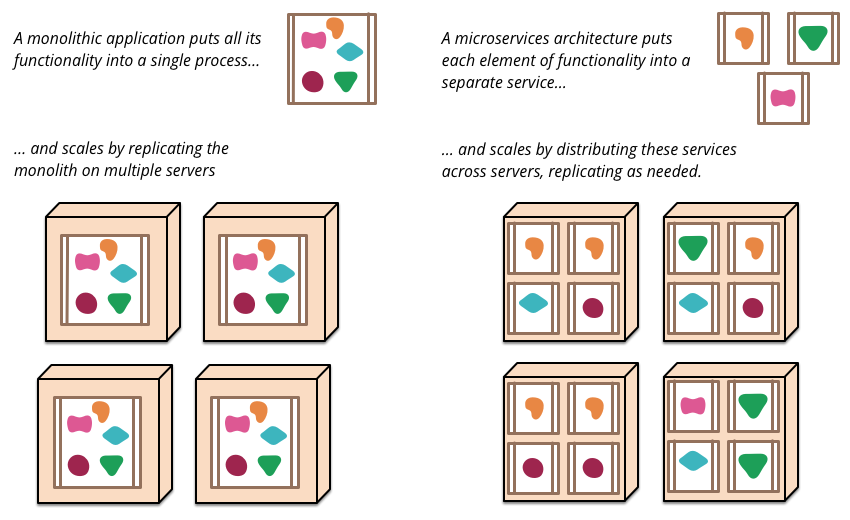
\includegraphics[scale=0.4]{pictures/sketch_microservices.png}
	    \end{center}
	    \label{fig:microsservicos_vs_monolito}
	    \legend{Fonte: https://martinfowler.com/articles/microservices/images/sketch.png}
	\end{figure}

    A arquitetura de microsserviços tem diversas vantagens em relação a monolítica, como por exemplo a divisão da lógica de negócio em pequenos serviços torna esses mais fáceis de compreender em relação a uma grande aplicação única. Esse modelo também torna mais simples a adoção de novas tecnologias sem a necessidade de intervir em serviços já existentes, isso acaba também por facilitar o desenvolvimento em equipe, dando mais independência para times entenderem e realizarem modificações em seus serviços, o que por fim contribui para o crescimento da empresa e sua escalabilidade.\cite{microservices-intro}
    
    Microsserviços também são uma opção altamente escalável e permitem que cada serviço seja dimensionando dinamicamente e individualmente em relação aos outros, o que significa que em arquiteturas de maior porte permite uma economia de recursos e melhor dimensionamento de capacidade dos serviços.
    
    Por outro lado, microsserviços também tem seu lado negativo, possuindo algumas desvantagens em relação ao modelo monolítico. Entre elas o sistema altamente distribuído exige que se tenha um alto nível de automação da infra-estrutura para que eles possam ser utilizados de forma fácil, como por exemplo o uso de algum PaaS. Gerenciamento de dados distribuídos, problemas de consistência eventual e lógica distribuída também se apresentam como desafios desse modelo de arquitetura.

	\section{Distributed Tracing}
	
	Distributed Tracing, ou Rastreamento Distribuído, é uma técnica utilizada em sistemas distribuídos para conseguir acompanhar algum fluxo que acaba por interagir com diversos serviços. Muito utilizado para ajudar desenvolvedor em sessões de depuração afim de entender qual caminho de código está sendo executado e com quais parâmetros em um sistema complexo e distribuído. Geralmente esse sistema se compõe de um broker central para onde as métricas e dados de tracing são enviados pelos serviços, e um conjunto de código que roda em todos os serviços, responsável por realizar a amostragem e enviar esses dados para o broker principal. Enquanto os brokers esperam receber mensagens representando eventos de entrada ou saída dos serviços através de um processo coletor, as bibliotecas se encarregam de enviar essa menagem e também propagar informações de rastreabilidade para as próximas interações com outros serviços. Podemos ver um digrama exemplificando a arquitetura de um Distributed Tracing nas figuras \ref{fig_tracing_concept} e \ref{fig_tracing_components}
	
	\begin{figure}[htb]
		\caption{\label{fig_tracing_concept}Anatomia de um Distributed Tracing}
		\begin{center}
		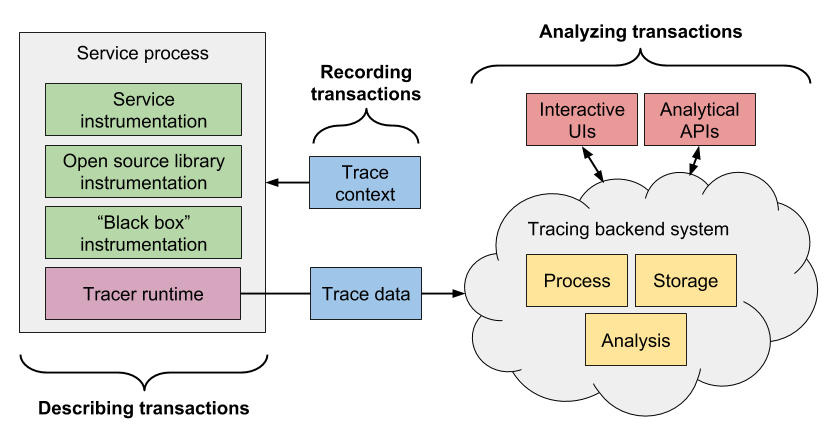
\includegraphics[scale=0.5]{pictures/tracing_concept.png}
		\end{center}
		\legend{Fonte: \url{https://cdn-images-1.medium.com/max/838/1*NuwuCvqZHLBJcJycRr1HTw.png}}
	\end{figure}
	
	\begin{figure}[htb]
		\caption{\label{fig_tracing_components}Componentes de um Distributed Tracing}
		\begin{center}
		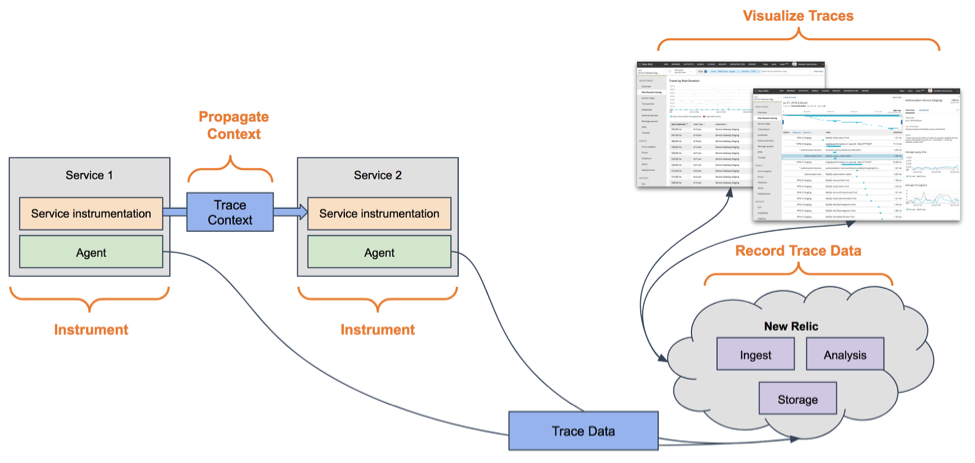
\includegraphics[scale=0.95]{pictures/distributed-tracing-components.png}
		\end{center}
		\legend{Fonte: \url{http://blog.newrelic.com/wp-content/uploads/Distributed-tracing-components.png}}
	\end{figure}
	
	Um dos primeiros Distributed Tracers que foi desenvolvido, foi o Dapper \cite{googledapper}, pela Google em meados de 2010. Com a abertura do código do Dapper outras empresas acabaram se interessando pelo projeto e funcionalidades e criaram suas próprias versões de tracers, entre eles alguns dos mais famosos: Zipkin\cite{zipkin}, pelo Twitter, e Jaeger\cite{jaegerarch}, pela Uber. Com o surgimento de novos tracers no mercado, a industria entrou em busca de um padrão para esse tipo de software, originando-se o OpenTracing\cite{opentracing}. OpenTracing é um padrão desenvolvido afim de definir normas e regras e padrões para implementação de Distributed Tracers. Nela são descritos estratégias para se realizar a identificação de informações gera mente importantes e o formato do tráfego de dados entre os serviços e os brokers.
	
	Grande parte do valor dos Distributed Tracing vem de suas ferramentas analíticas, que facilitam a vida do desenvolvedor e permitem com que ele faça análises de forma rápida e eficiente nos sistemas. Geralmente essas ferramentes vem junto com uma aplicação de Frontend que consegue exibir fluxos e montar gráficos. Entre eles o Flamegraph é muito utilizado para visualizarmos como a comunicação se aprofunda e se propaga na rede, uum exemplo de Flamegraph do Zipkin pode ser visto na figura \ref{fig_zipking_sample}. Outro tipo de visualização muito útil é a de mapa de Topologia de servços, que nada mais é que um grafo representando as interações entre diversos serviços, temos um exemplo na figura \ref{fig_topology_map}
	
	\begin{figure}[htb]
		\caption{\label{fig_zipking_sample}Exemplo de Flamegraph do Zipkin}
		\begin{center}
		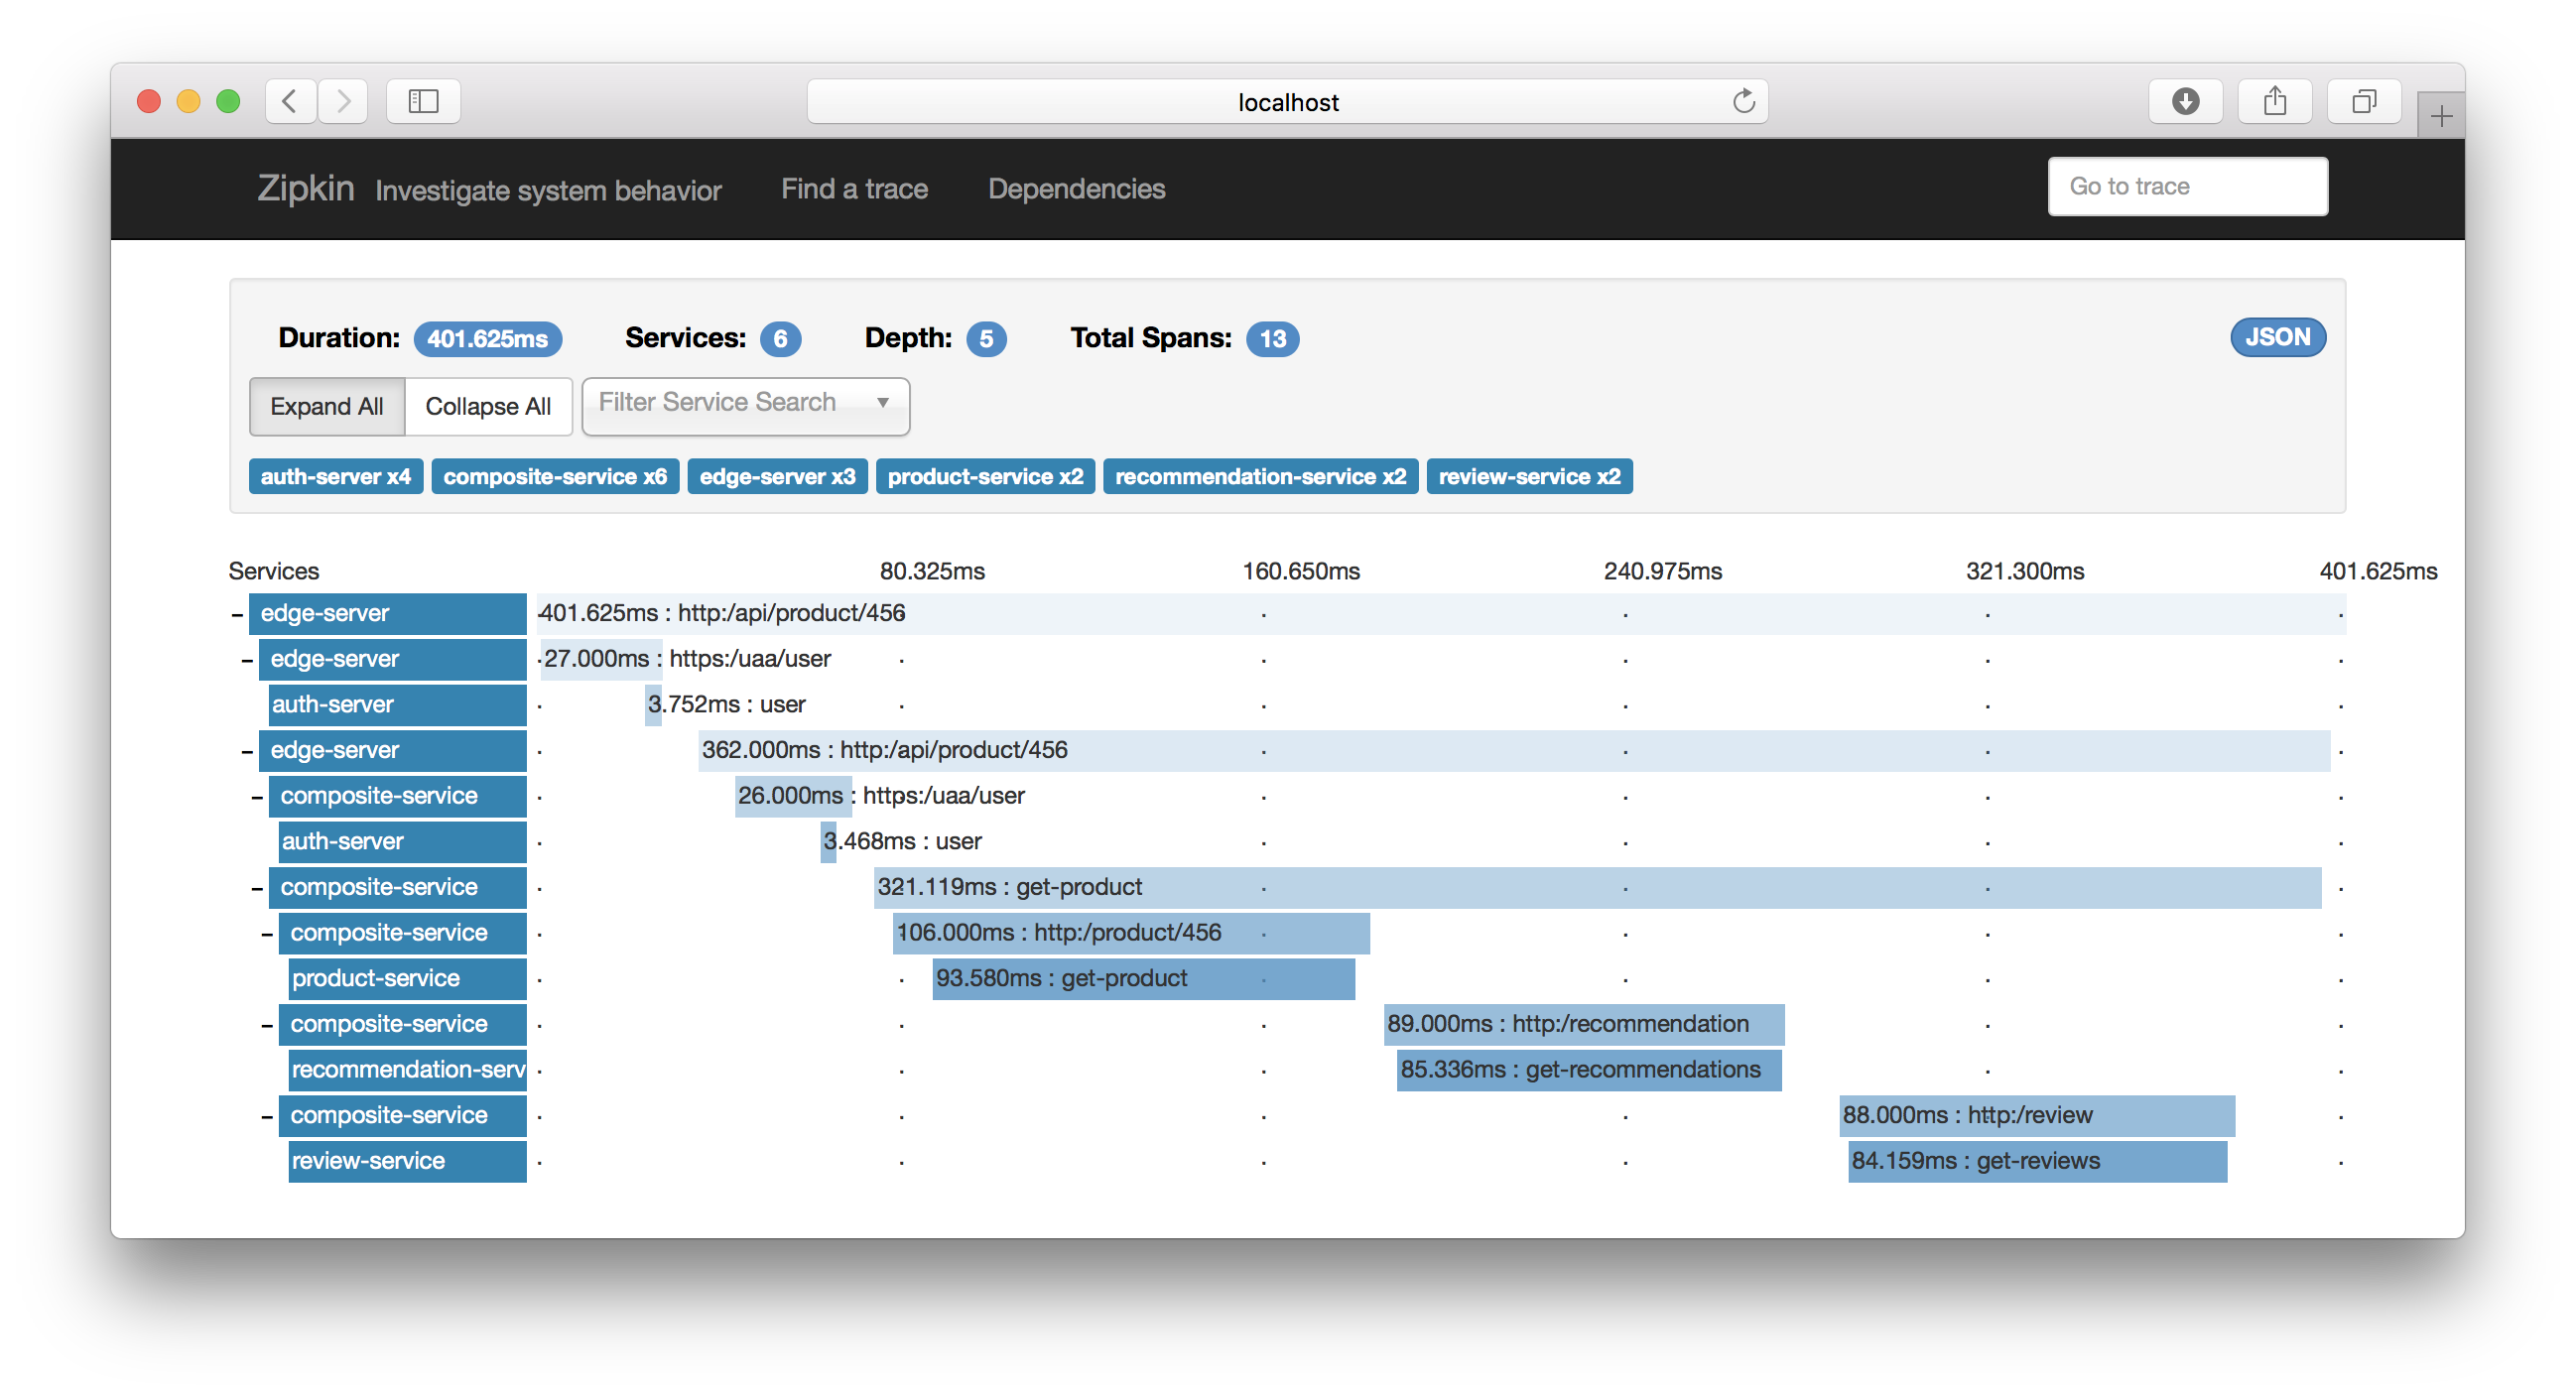
\includegraphics[scale=0.16]{pictures/zipkin-sample.png}
		\end{center}
		\legend{Fonte: \url{http://callistaenterprise.se/assets/blogg/build-microservices-part-7/Zipkin-sample.png}}
	\end{figure}
	
	\begin{figure}[htb]
		\caption{\label{fig_topology_map}Exemplo de Mapa de Topologia de Serviços}
		\begin{center}
		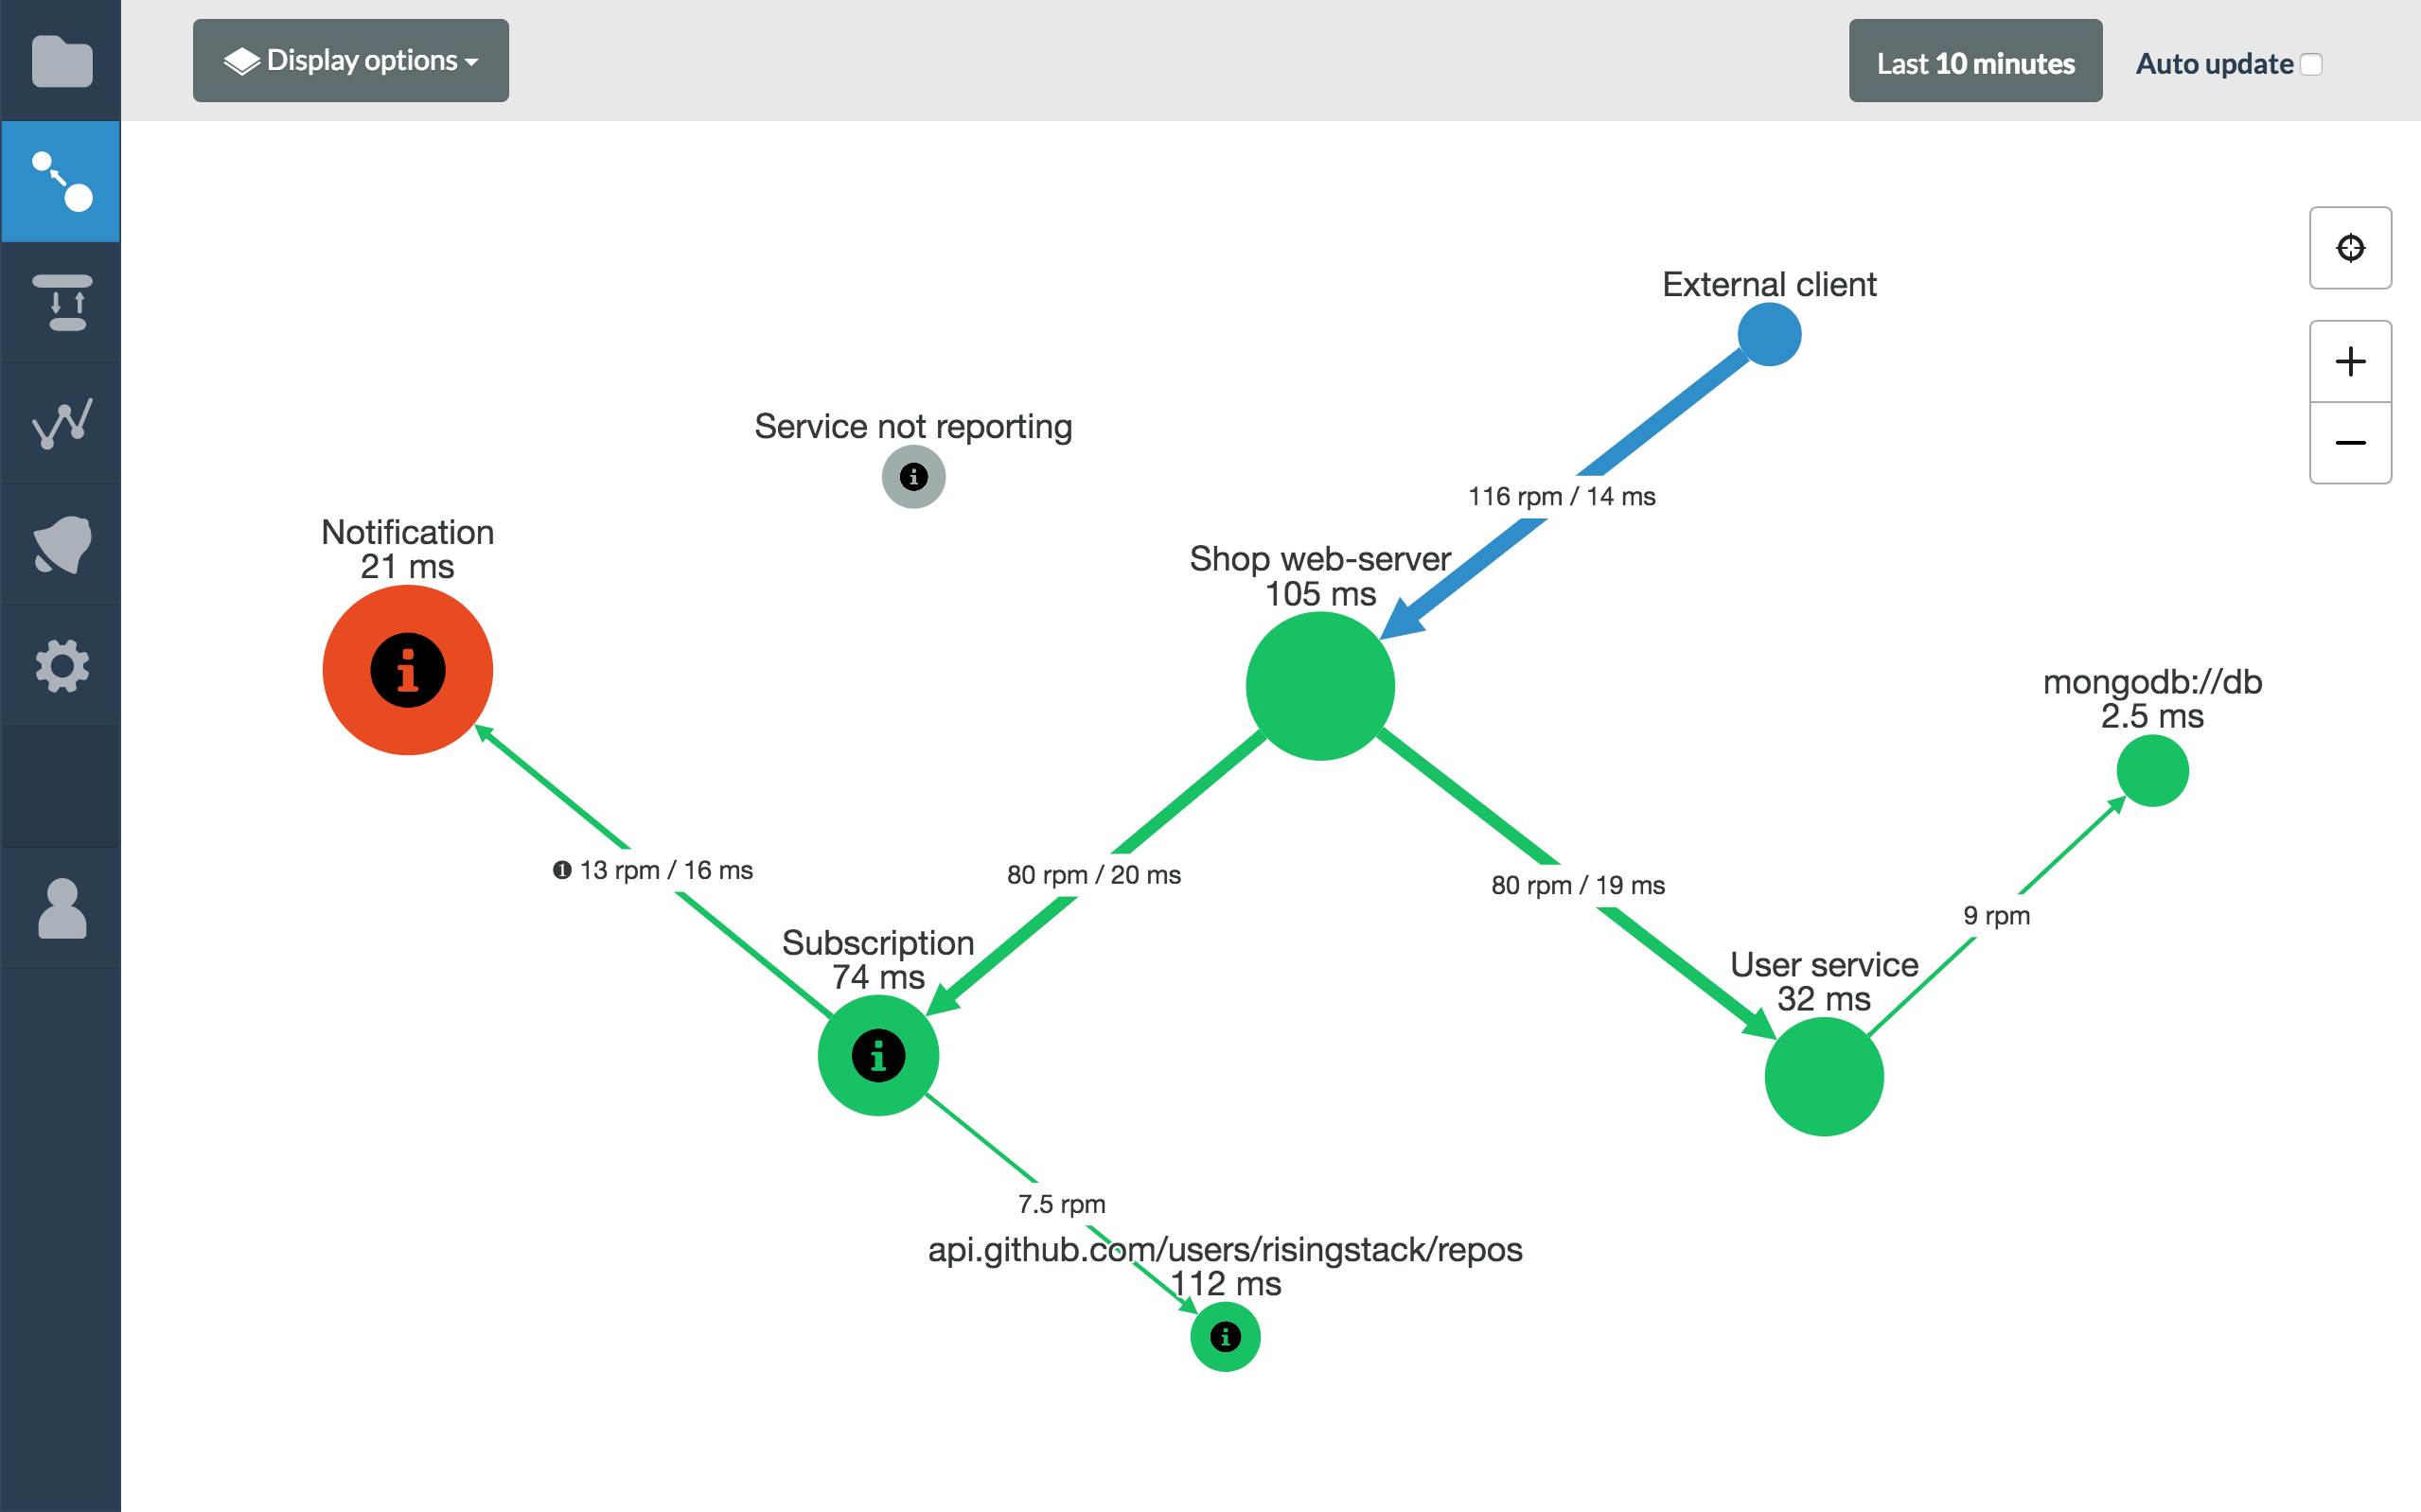
\includegraphics[scale=0.16]{pictures/service_topology_map.png}
		\end{center}
		\legend{Fonte: \url{https://blog-assets.risingstack.com/2016/May/Distributed_transaction_tracing_with_service_topology_map_trace_by_risingstack-1462456507669.png}}
	\end{figure}
	
	\section{Devspaces}
    
    Um Devspace, como foi batizado pelo grupo, é um ambiente de desenvolvimento isolado que roda em cima da plataforma Formicarium. Ele é o ambiente que o desenvolvedor vai ter disponível para uso e que vai interagir durante o seu tempo testando e desenvolvendo os serviços. 
    
    Os Devspaces são provisionados e configurados de forma automática pelo serviço Soil, a medida que um desenvolvedor requisita sua criação através da CLI. Para obter dados de configuração e setup inicial do Devspace, o Soil consulta um servidor de configurações via Webhooks, esse encarregado de fornecer todo configuração específica da empresa para fazer o bootstrap de um novo Devspace.
    
    Objetivamente, os Devspaces são Namespaces do Kubernetes que são gerenciados pelo Soil, além dos recursos padrões do Kubernetes, esse Namespaces acabam recebendo serviços adicionais do Formicarium, sendo esses o Hive e o Tanajura. A interação com os Devspaces é feito sempre através da CLI do Formicarium, não exigindo que o usuário tenha que ter o ferramental do Kubernetes instalado e configurado em sua máquina.
    
    Dentro de um Devspace os serviços que rodam nele conseguem se localizar entre si por meio do servidor de DNS do Kubernetes que garante isolamento entre Namespaces, dessa forma conseguimos alcançar um isolamento entre serviços entre Devspaces, mesmo que 2 desenvolvedores estejam executando o mesmo serviço. Além disso, cada Devspace recebe do Config Server um conjunto de aplicações de infra-estrutura ou de uso comum, que também garante isolamento dos demais Devspaces, como por exemplo, a existência de um broker de mensageria por Devspace. não havendo confusão na produção e consumo de mensagens.
    
        \begin{figure}[htbp]
			\caption{\label{fig_devspace1}Anatomia de um Devspace}
			\begin{center}
			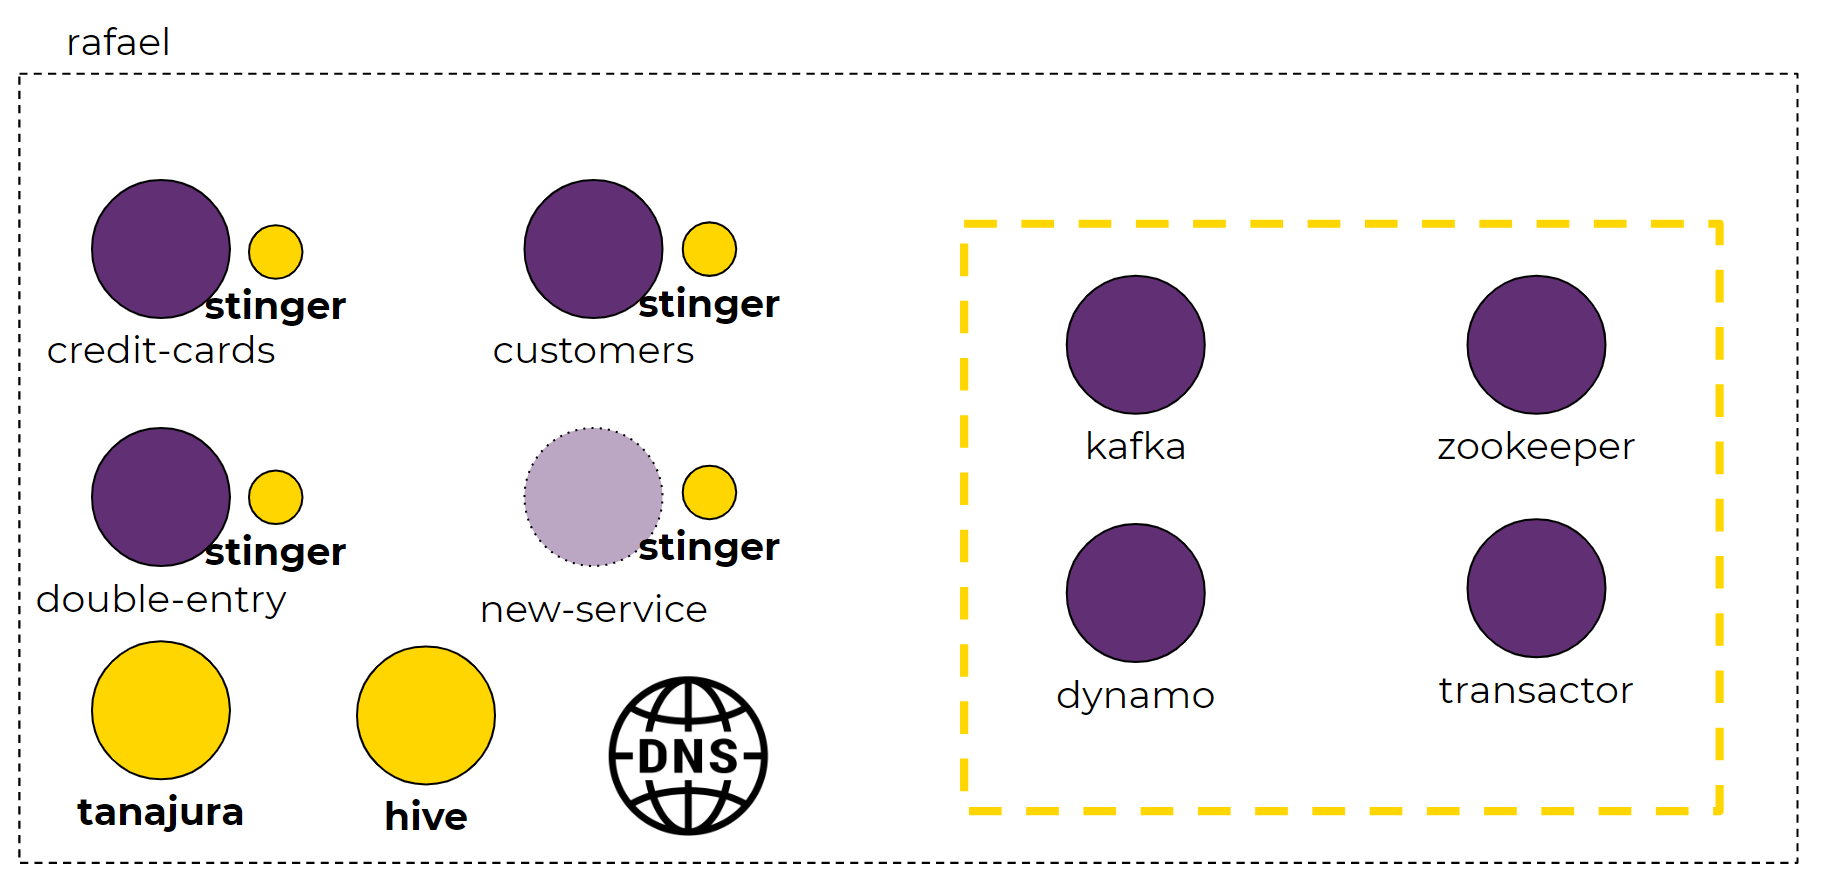
\includegraphics[scale=0.30]{pictures/devspace1.png}
			\end{center}
			\legend{Fonte: os autores}
			% \caption{Fonte: própria}
		\end{figure}
    
    	\begin{figure}[htbp]
			\caption{\label{fig_create_devspace}Fluxo de Criação de Devspaces}
			\begin{center}
			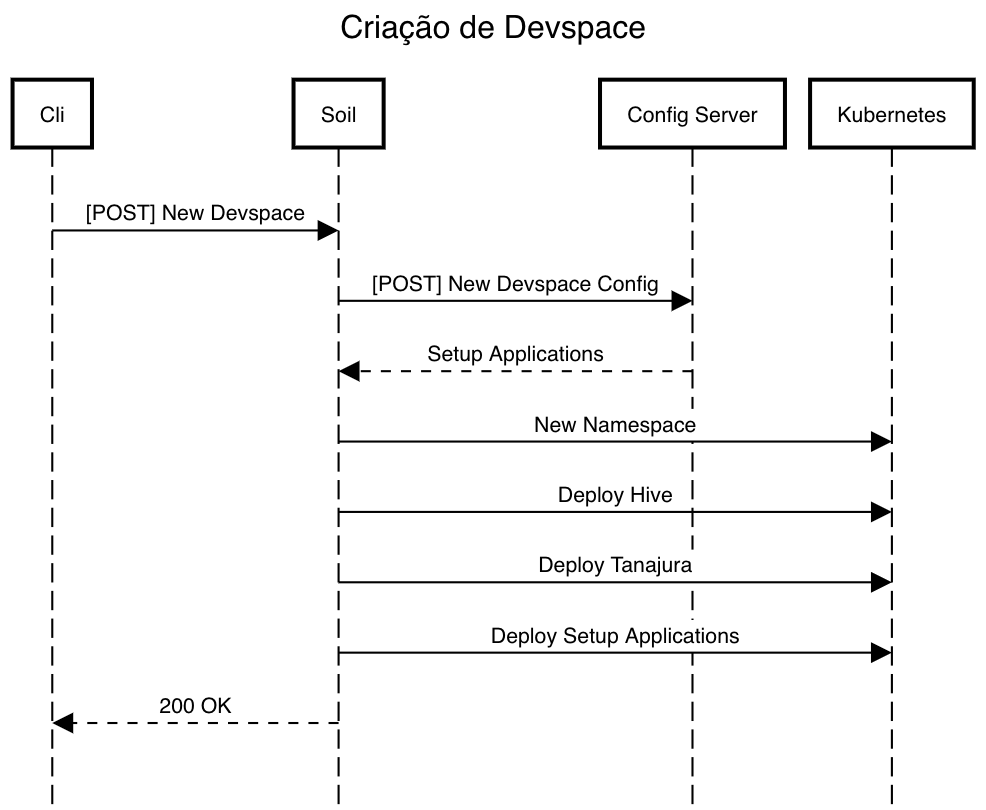
\includegraphics[scale=0.40]{pictures/create-devspace.png}
			\end{center}
			\legend{Fonte: os autores}
			% \caption{Fonte: própria}
		\end{figure}
 
\chapter{Tecnologias Utilizadas}
    \section{Protocolos de Comunicação}
        \subsection{HTTP}
	    Acrônimo de \textit{HyperText Transfer Protocol}. Protocolo usado pela \textit{Web}, define formato de mensagens trafegadas e formatação, dando também orientações semânticas via códigos\cite{httpcodes} de como os \textit{browsers} ou servidores devem reagir em resposta a diversos comandos.
	
	    \subsection{Git}
	        Git é um sistema de controle de versões distribuído amplamente utilizado em desenvolvimento de software. o Git se organiza através de repositórios que podem ser clonados e editados localmente pelo usuário e então sincronizados com um servidor remoto, publicando as alterações. Todo o histórico de alterações é mantido nesse processo sem perda de informações.
	        
	        Alguns conceitos importantes de serem destacados no funcionamento do Git para o melhor entendimento desse projeto são os seguintes:
	
        	\textbf{Repositório}
        	\newline
        	Corresponde a um diretório de arquivos gerenciado pelo Git.
        	
        	\textbf{Commit}
        	\newline
        	É uma consolidação de um conjunto de alterações realizado no repositório Git. Representa um ponteiro para um estado específico (uma versão).
        	
        	\textbf{Branch}
        	\newline
        	Branch é um ponteiro movél que aponta para um determinado commit. Branches criam a ideia de uma árvore de caminhos em um repositório apontam sempre para o commit mais recente de uma bifurcação de mudanças.
        	
        	\textbf{HEAD}
        	\newline
        	HEAD é um ponteiro que aponta para para o branch ou commit atual que está em uso no repositório local.
        	
        	\textbf{FETCH\_HEAD}
        	\newline
        	Um ponteiro efêmero que aponta para a última referência buscada por um fetch.
        	
        	\textbf{Staging}
        	\newline
        	Área do Git onde as alterações que vão entrar no próximo commit ficam
        	
        	\begin{figure}[htbp]
        		\caption{\label{fig_git1}Anatomia do Git}
        		\begin{center}
        		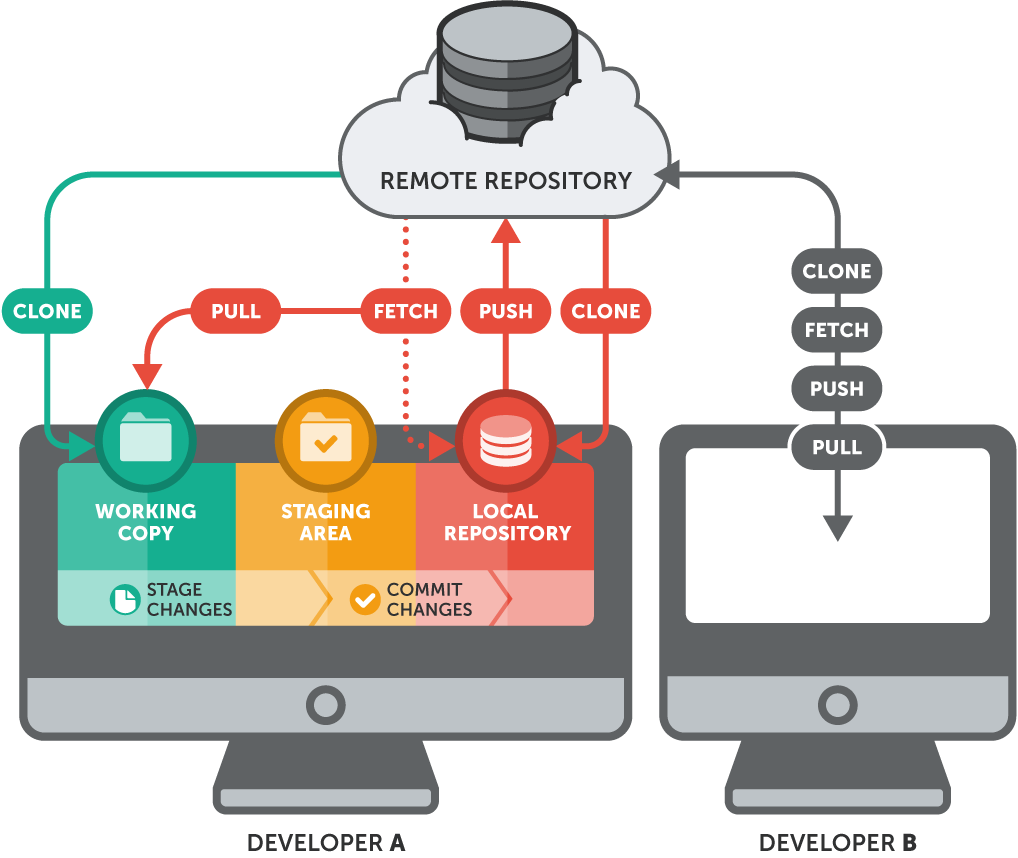
\includegraphics[scale=0.4]{pictures/git.png}
        		\end{center}
        		\legend{Fonte: \url{https://raw.githubusercontent.com/UnbDroid/AprendendoGithub/master/images/git.png}}
        	\end{figure}
        	
        	Para realizar a sincronização entre repositórios locais e remotos o Git possibilita o uso de diversos protocolos de rede, temos entre eles principalmente: HTTP(S), FTP, rsync ou SSH.
        	
        	Durante o processo de uso do Git algumas ações são frequentemente utilizadas, e valem ser destacadas aqui, essas são:
        	\begin{itemize}
            	\item \textbf{git init:} 
            	Inicia um repositório git vazio no diretório.
            	
            	\item \textbf{git clone:}
            	Cria um cópia de um repositório remoto localmente, acaba por fazer um download da estrutura remota para a maquina do usuário.
            	
            	\item \textbf{git fetch:}
        	    Sincroniza o estado do repositório remoto com o local sem realizar alterações na \textit{working tree} do desenvolvedor. Baixa os dados existentes no repositório remote que não existem no computador do usuário.
        	
            	\item \textbf{git checkout:}
            	Alinha o repositório local de acordo com a revisão ou branch especificado no comando.
            	
            	\item \textbf{git commit:}
            	O commit é o ato de criar um ponto no histórico do repositório contendo as mudanças que foram adicionas na área de staging.
            	
            	\item \textbf{git add:}
            	O comando \textit{add} é responsável por adicionar as mudanças especificadas na área de staging do git para serem comitadas em seguida.
            	
            	\item \textbf{git push:}
            	O push executa a ação de enviar os commits locais para o repositório remoto especificado.
            	
            	\item \textbf{git merge:}
            	Atualiza os arquivos na working tree para corresponderem ao especificado no comando. O merge também pode acabar atualizando o HEAD do branch atual.
            	
            	\item \textbf{git pull:}
            	Esse comando realiza a atualização do repositório local a partir das mudanças realizadas no repositório remoto. De forma geral ele acaba realizando um download dos commits mais recentes que estão presentes no remote. É uma combinação do git fetch com o git merge FETCH\_HEAD
        	\end{itemize}
        	\begin{figure}[htb]
        		\caption{\label{fig_git2}Fluxo de trabalho em Git}
        		\begin{center}
        		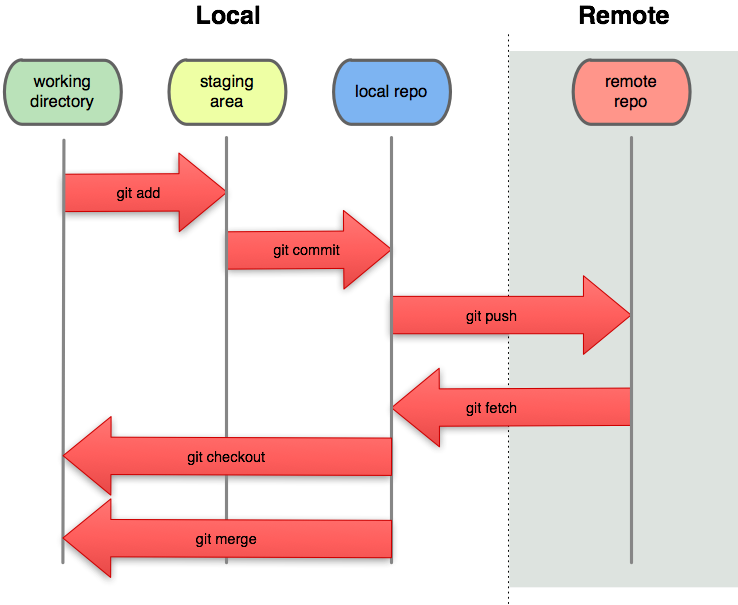
\includegraphics[scale=1]{pictures/GIT2.png}
        		\end{center}
        		\legend{Fonte: \url{https://kevintshoemaker.github.io/StatsChats/GIT2.png}}
        	\end{figure}
        	
    	\subsection{GraphQL}
            GraphQL é uma linguagem de consulta criada pelo Facebook em 2002 e lançada publicamente em 2015. É utilizada principalmente em conjunto com o protocolo HTTP no contexto de um servidor web para que um cliente possa obter os dados que necessita de um servidor.
            Ele tem algumas características que torna seu uso interessante, como por exemplo:
            - Ela permite que o cliente especifique exatamente quais dados ele quer que sejam retornados em determinada requisição
            - Torna fácil o processo de agregação de dados vindos de diferentes fontes.
            - Utiliza um sistema de tipos para descrever dados.
    
            Além disso, a comunidade oferece diversos \textit{Frameworks} que atuam no lado do cliente e que são responsáveis pela obtenção, cacheamento e normalização dos dados. Os mais relevantes são Apollo e Relay (também desenvolvido e mantido pelo Facebook). Do lado do servidor, existe uma infinidade de implementações de GraphQL nas mais diferentes linguagens de programação, sendo a mais popular a implementação de referência em Javascript, mantida pela própria empresa criadora da linguagem.
        
            GraphQL é uma alternativa ao modelo REST e vem ganhando espaço no mercado nos últimos anos, sendo utilizado por grandes empresas como Facebook e Github em seus produtos mais importantes.
    
        \subsection{ZeroMQ} 
        
        ZeroMQ é um biblioteca escrita originalmente em C que provê a ferramentas para a construção de mecanismos de rede embarcada em aplicações diversas. Ela fornece diversos tipos de \textit{sockets} que carregam mensagens atômicas através de diversos protocolos de transporte, como por exemplo TCP. O ZeroMQ possibilita a criação de topologias e padrões de conexão de \textit{sockets} extremamente variáveis e flexíveis, entre eles \textit{fan-out}, \textit{pub-sub}, \textit{request-reply}, entre outros. A implementação do ZeroMQ se utiliza de um modelo de I/O assíncrono que permite fácil escalabilidade e uma grande quantidade de carga. ZeroMQ tem bibliotecas em implementações na grande maioria das linguagens de programação, tornando ele um boa opção para arquiteturas mistas.\cite{zeromqguide}
        
    \section{Linguagens de Programação}
    	\subsection{Clojure}
    	    Clojure é uma linguagem de programação dinâmica e funcional. Sendo um dialeto de LISP que roda na JVM, é uma linguagem compilada, mas que mantém todas características dinâmicas a ser utilizadas em Runtime. Possui compatibilidade e interoperabilidade com todo ecossistema Java e de outras linguagens que rodem na JVM. Clojure enfatiza o uso de estruturas de dados imutáveis e de a filosofia de Code is Data, com um sistema poderoso de macros e de estruturas de dados mutáveis Thread Safe quando necessário. \cite{clojurerationale}
	
    	    Clojure é a principal linguagem de programação utilizada no Nubank, e também é muito familiar para o grupo, além de apresentar características interessantes para o desenvolvimento do projeto. como a grande habilidade para lidar com problemas de concorrência de forma segura e eficiente.
	
	        Dentro do desenvolvimento do projeto Clojure foi utilizada como uma das principais linguagens de programação para serviços de Backend. Um dos recursos que torna Clojure especialmente interessante é a possível interação em tempo real com o código através de um REPL (Read Eval Print Loop), algo que foi utilizado em um dos módulos do projeto como será descrito mais a frente. Além disso a familiaridade dos desenvolvedores do Nubank com a linguagem foi um fator decisivo para que o projeto pudesse continuar a ser mantido por mais pessoas no futuro.
	
        	\begin{figure}
        	    \centering
        	    
\includegraphics[scale=0.1]{pictures/clojure_logo.png}
        	    \caption{Logo Clojure}
        	    \legend{Fonte: \url{https://cdn-images-1.medium.com/max/1200/1*eLqeIits5crU3G5b9LMEyg.png}}
        	    \label{fig:logo_clojure}
        	\end{figure}
	
        \subsection{Javascript} %% TODO: Paps
            Javascript é uma linguagem de programação interpretada baseada em ECMAScript. Foi originalmente criada para atuar junto com navegadores web, tornando possível que scripts fossem executados no lado do cliente sem passar pelo servidor, realizando comunicação assíncrona (AJAX) a manipulando o conteúdo do documento exibido em páginas web.
            
            Ela foi concebida par ser uma linguagem script com orientação a objetos baseada em protótipos, tipagem fraca e dinâmica e funções de primeira classe. Possui suporte à programação funcional e apresenta recursos como \textit{Closures} e \textit{higher-order functions}.

            Hoje é uma das linguagens mais populares do mundo e já há alguns anos vem sendo bastante utilizada no lado do servidor através de ambientes como Node.js. 
	
	
            \subsubsection{Typescript}
                Typescript é uma linguagem de programação desenvolvida e mantida pela Microsoft que tem como objetivo tornar bases de código em Javascript mais fáceis de se manter e menos suscetíveis à erros, através da adição de um sistema de tipos à linguagem, entre outros recursos. 

                Para que o código escrito em Typescript possa de fato ser executado em ambientes como navegadores web e Node.js, é preciso compilá-lo para Javascript e este processo pode ser feito através do compilador oferecido como parte do ferramental da linguagem. Na verdade, todo código Javascript é um código Typescript válido, porém o contrário não é verdadeiro.

            \subsubsection{Node.js}
                Node.js é um ambiente de execução multiplataforma e de código aberto, com a capacidade de executar Javascript fora do contexto de um browser, tornando possível o uso da linguagem em um ambiente de servidor.
    
                Utiliza o motor de Javascript V8, desenvolvido pela Google e que está presente também em seu navegador Google Chrome. Node.js segue uma arquitetura \textit{event-driven} capaz de realizar I/O de maneira assíncrona e não bloqueante. Estas escolhas de projeto tem como objetivo otimizar o \textit{throughput} e escalabilidade em aplicações web com muitas operações de entrada e saída, bem como aplicações web \textit{real-time} como por exemplo programas de comunicação em tempo real e jogos.

                Como parte de seu ecossistema, é oferecido um gerenciador de pacotes chamado \textit{npm}, que conta com uma interface de linha de comando e um banco de dados público de pacotes, que podem ser adicionados em projetos através de um sistema de dependência.

                Hoje Node.js é utilizado por empresas como GoDaddy, Groupon, IBM, Linkedin, Microsoft, Netflix, PayPal, Rakuten, Walmart, Yahoo, entre outros.

    \section{React}
        React é uma biblioteca JavaScript de código aberto para criar interfaces interativas. É declarativa, eficiente e flexível e permite que o desenvolvedor componha interfaces complexas a partir de partes menores e isoladas chamadas "componentes".

        Utiliza a técnica de \textit{Virtual DOM}, o que melhora drasticamente sua performance pois diminui o número de operações feitas de fato no DOM (\textit{Document Object Model}), que costumam ser tarefas de processamento mais intensivo.

	
	\section{Docker}
	    Docker é uma plataforma \textit{open source} para desenvolvimento de aplicações através de contêineres, criada e mantida pela empresa Docker Inc. Foi escrito na linguagem de programação Go, que é fortemente tipada e possui \textit{garbage collector} para gerenciamento de memória, além de suporte explícito para programação concorrente.
	
	    No seu ecossistema existem ferramentas para criação de imagens e execução de con\-têi\-ne\-res (\textit{Docker Engine}), repositórios para distribuição de imagens (\textit{Registries}) e também uma ferramenta para orquestração de con\-têi\-ne\-res em um cluster (\textit{Docker Swarm})
	
	
    	\subsection{Base tecnológica}
    	    O Docker se utiliza de diversos recursos do kernel do sistema operacional para prover a tecnologia de contêineres, como \textit{cgroups}, que permitem que os processos sejam organizados em grupos hierárquicos e cuja utilização de recursos pode ser limitada e monitorada. \textit{Namespaces}, que permitem que um sistema isole uma coleção de processos para que não possam ver certas partes do sistema geral e o \textit{Unionfs}, que é um sistema de arquivos empilhável que permite aos usuários especificar um conjunto de diretórios que são apresentados como um único diretório virtual, mesmo que estes possam vir de diferentes sistemas de arquivos.
    	
    	\subsection{Arquitetura}
    	    Utiliza-se de uma arquitetura cliente-servidor composta por três componentes: um \textit{Daemon}, que é o responsável por criar e manipular os objetos Docker (imagens, contêineres, redes, volumes, \textit{etc.}) e age como servidor.
    	
    	    Uma API REST, que define uma interface que os outros programas podem utilizar para interagir com o daemon e instruí-lo sobre o que fazer.
    	
    	    Uma interface de linha de comando, que é a principal interface do usuário com o Docker. Ela age como cliente e se utiliza da API REST para interagir com o daemon através de scripts ou diretamente de comandos em um terminal.
    	
    	\subsection{Objetos Docker}
    	    \subsubsection{Imagens}
    	        Uma imagem é um \textit{template read-only} com instruções para a criação de um contêiner Docker. Normalmente é baseada em outra imagem, com customizações adicionais. Por exemplo, é possível construir uma imagem baseada na imagem do \texttt{ubuntu}, porém que instala e configura um servidor web Apache e uma determinada aplicação.
    	
    	        Para criar uma imagem, é preciso um Dockerfile, arquivo que se utiliza de uma sintaxe simples para definir os passos necessários para criar a imagem e executá-la. Cada instrução em um Dockerfile cria uma camada na imagem, que são reaproveitadas quando a imagem é reconstruída caso a instrução continue a mesma. Esta estratégia é responsável por tornar as imagens leves e rápidas, quando comparadas com outras tecnologias de virtualização.
    	
        	\subsubsection{Contêineres}
        	    Um contêiner é uma instância executável de uma imagem. É possível criar, pausar, interromper, mover e remover um contêiner utilizando a interface de linha de comando ou a API REST. É possível também conectar um contêiner em uma ou mais redes, acoplar volumes de dados ou mesmo gerar novas imagens a partir do estado atual de um contêiner.
        	
    	        Por padrão, um contêiner é relativamente bem isolado de outros contêineres e da máquina hospedeira, e este nível de isolamento pode ser controlado através dos mecanismos de redes e volumes oferecidos pelo Docker.
    	
    	        Um contêiner é efêmero do ponto de vista que nenhuma das mudanças em seu estado que não forem armazenadas de maneira persistentes serão perdidas assim que o contêiner é removido. \cite{dockeroverview}
	
	
	\section{Kubernetes}
	    Kubernetes é um projeto de código aberto da Google, que possui mais de 1800 contribuidores e ganha cada vez mais atenção no mundo de operação e desenvolvimento de software. 
	    A Google, dado a escala de sua operação, sofria com problemas com o gerenciamento de muitas máquinas virtuais. 
    	Assim, precisou-se repensar como lidar com esse problema, o que, depois de anos, levou ao gerenciador e escalonador de contêineres chamado Kubernetes.

    	Para entender melhor a necessidade de um gerenciador tal como o Kubernetes, é necessário dar um passo atrás e olhar para as vantagens e desvantagens dos contêineres.
    	Contêiners são feitos para serem leves, rápidos, mas de duração curta e frágeis.
    	Assim, eles trocaram a resiliência de uma máquina virtual pela velocidade e leveza. Isso requer que contêineres rodem em um ambiente onde em caso de falha ou mudança de carga, esse ambiente garanta a substituição desses contêineres e gerencie eventuais mudanças de rede e recursos de memória e CPU do \textit{cluster}.
    	
    	Kubernetes trabalha com a ideia de guardar o estado desejado do \textit{cluster}. Isso porque, em sistemas distribuídos, é importante a construção de um modelo de estado global.\cite{globalstate} Muitos problemas são resolvidos com uma boa modelagem de estado global. Para isso, o Kubernetes provê alguns objetos através da sua API. Dentre todos os objetos, os relevantes para o nosso projeto são:
    	
	    \begin{itemize}
	        \item \textit{Namespace}: provêm um escopo de nomes, são projetados para ambientes nos quais há diversos usuários do \textit{cluster}. Recursos dentro de um namespace devem ter um nome único.\cite{k8sdocsnamespace}
	        \item \textit{Pod}: respresenta a unidade mais simples capaz de ser distribuída pelo Kubernetes. É o bloco básico para construção de outros objetos. Encapsulam um ou mais contêineres que representam uma aplicação, com todos os requisitos de disco e rede. Pods são efêmeros, isto é, eles podem ser removidos e recriados sem aviso prévio. \cite{k8sdocspods}
	        \item \textit{Deployment}: é um dos objetos controladores, provém atualizações declarativas aos \textit{Pods}. Capaz de criar e gerenciar réplicas de Pods, \textit{rollout} de atualizações, reinício de \textit{Pods} em caso de falha. \cite{k8sdocsdeployments}
	        \item \textit{Service}: é uma abstração que define um conjunto lógico de \textit{Pods} e uma política de acesso a ele.\cite{k8sdocsservice} Quando um \textit{Service} é criado dentro de um \textit{Namespace}, é criado uma entrada de DNS, permitindo que os \textit{Pods} se encontrem na rede apenas pelo nome do \textit{Service}, garantindo que com a mesma configuração, serviços acessem recursos de seus respectivos \textit{Namespaces}. \cite{k8sdocsnamespace}
	        \item \textit{Ingress}: são configurações de acesso externo ao \textit{cluster}, tipicamente HTTP. \cite{k8sdocsingress} 
	    \end{itemize}


\chapter{Metodologia do Trabalho}
    \section{Introdução}
        A nossa metodologia de trabalho foi uma adaptação da proposta de (Bittner, 2002)\cite{usecases}, ODP() e Scrum\cite{essentialscrum}. Tendo entendido o problema e o \textit{stakeholders} (primeira parte), Unimos a completeza e formalidade da definição de requisitos funcionais identificáveis por casos de uso e ODP para a concepção inicial do produto (segunda parte), inserindo esses conhecimentos num \textit{framework} de \textit{Scrum}, adaptado para o nosso contexto (terceira parte).
        
        \begin{enumerate}
            \item Definição de stakeholders e contexto do problema
            \item Concepção inicial do produto
            \item Execução iterativa
        \end{enumerate}

    \section{Definição de Stakeholders e contexto do pro\-ble\-ma}
        Um stakeholder é uma pessoa ou organização com direitos ou interesse com respeito ao sistema ou às propriedades dele. Os \textit{stakeholders} dão forma ao software, gerando oportunidades e limitações ao desenvolvimento, sendo também a fonte de requisitos do sistema. Os desenvolvedores podem propor requisitos, mas cabe aos \textit{stakeholders} acatar as sugestões ou não.

        A tabela \ref{tab:roles} mostra os \textit{stakeholders} de nosso projeto, e em seguida temos uma descrição das dores e influência de cada um na nossa solução. O método de alinhamento de expectativas está descrito na próxima seção.

        \begin{table}[ht]
            \centering
            \caption{Papéis de cada entidade ao longo do projeto.}
            \begin{tabular}{l l}
                Entidade                            & Papel \\
                \hline
                Leonardo Iacovini                   &  Desenvolvedor, stakeholder  \\
                Luiz Gustavo                        &  Desenvolvedor, stakeholder  \\
                Rafael Leal                           &  Desenvolvedor, stakeholder \\
                Rafael Correia                      &  Desenvolvedor, stakeholder \\
                Rafael Ferreira                     &  Stakeholder \\
                Integrantes da equipe de platform   &  Stakeholder \\
                Integrantes da equipe de lending    &  Stakeholder 
            \end{tabular}
            \label{tab:roles}
        \end{table}
        \subsection{Detalhamento dos stakeholders e influências}
            TBD

    \section{Concepção inicial do produto}
        \subsection{ODP}
        \subsection{Outras considerações}

    \section{Execução Iterativa}
        Simplificamos muitas das práticas do \textit{scrum} usual para lidar com as limitações e o menor escopo do projeto, se comparado com desenvolvimento de software empresarial de larga escala.
        
        Usamos \textit{sprints} de duas semanas cada, correspondente ao período de implementação do que foi definido como prioridade, a partir do \textit{backlog}. Este, por sua vez, fora definido em cada uma das reuniões de \textit{sprint planning}, usadas por nós para priorizar tarefas do \textit{backlog}, identificar os maiores problemas e travas para prosseguir na implementação e reorganizar e/ou atualizar os \textit{milestones}.\par
        
        Trabalhamos três vezes por semana, fazendo sessões de \textit{pairing} para codificar a solução e discuti-la e fazer \textit{live-testing} em reuniões de 4 horas a 6 horas de duração, em média, dependendo da dificuldade do problema que estávamos tentando resolver, ou disponibilidade dos integrantes do grupo.
        
        Como estávamos todos na mesma sala discutindo e implementando, ficou mais simples de difundir o conhecimento da arquitetura e das decisões de projeto para cada integrante, e problemas técnicos ou arquiteturais foram resolvidos com bastante eficiência, pois os outros integrantes estavam ao lado, caso qualquer dúvida ocorresse. Devido ao teor organizacional dessas reuniões de projeto que fizemos, vimos que as \textit{daily meetings} propostas pela metodologia de \textit{scrum} seriam supérfluas para nosso método de trabalho, e acabamos não adotando-as.
        
        Não coincidindo necessariamente com o final da \textit{sprint}, fizemos reuniões que uniram as idéias de \textit{sprint reviews} e \textit{sprint retrospective} para mostrar \textit{demo} aos nossos \textit{stakeholders}, pegar feedback e reorganizar o \textit{backlog} segundo o feedback dos mesmos, além de identificar o que deu errado, para poder se preparar melhor para o próximo período de trabalho. 
        
        Vale mencionar também que antes de termos a ideia do produto formalizada também fizemos algumas reuniões com um de nossos \textit{stakeholders} (Rafael Ferreira) que nos deu grande ajuda para entendermos do que se tratava o produto, além de proporcionar feedbacks quanto ao andamento do projeto, soluções técnicas e \textit{milestones}.
        
        Escolhemos não ter \textit{scrum master} pois o papel do mesmo de filtrar forças distrativas no nosso trabalho não se mostrou necessário, e também não tivemos \textit{Product Owner} pois o nosso \textit{backlog} foi feito de forma conjunta, pelos 4 desenvolvedores e a terceirização da comunicação com os \textit{stakeholders} não foi necessária, pois tínhamos liberdade e disponibilidade para falar com os mesmos diretamente, quando precisássemos.

    \section{Scrum } %% TODO: Luiz 
        Scrum\cite{essentialscrum} é um método de desenvolvimento de produtos e serviços. Esse método teve concepção em 1986, Em uma publicação\cite{scrumorigin} de Takeuchi e Nonaka, que descrevem bons resultados obtidos em grandes empresas usando a metodologia.
        
        O início da execução do \textit{Scrum} é criar uma lista priorizada de \textit{features} (funcionalidades) e outras capacidades necessárias pra se desenvolver um produto com sucesso, chamada de \textbf{backlog}. A implementação sempre tem que seguir a ordem de prioridade atribuída a cada \textit{feature}, sendo sempre executado primeiro o que for mais prioritário.
        
        O trabalho é feito em \textit{Sprints}: iterações de tempo curto e limitado (em geral de 1 ou 2 semanas). A execução é feita por uma equipe multi-funcional e auto-contida, com desenvolvedores, arquitetos, engenheiros, \textit{designers}, etc, de modo que ao final da \textit{Sprint} obtém-se uma parte do produto que traz algum valor de negócio.
        
        No final da \textit{Sprint}, a equipe revisa o que foi feito com os \textit{stakeholders} e ajusta a priorização de acordo com o \textit{feedback}. O ciclo recomeça com uma reunião de planejamento para a próxima iteração.
        
        \begin{figure}[htb]
    		\caption{\label{fig:scrum} Framework do scrum}
    		\begin{center}
    		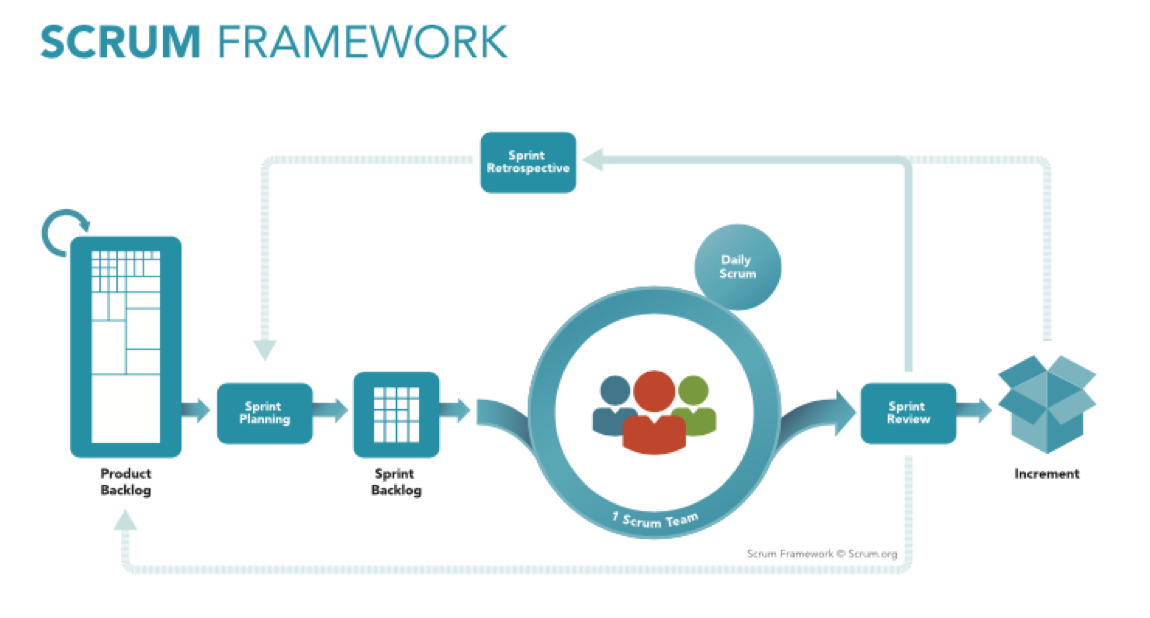
\includegraphics[width=\textwidth,keepaspectratio]{pictures/ScrumFrameworkTest.png}
    		\end{center}
    		\legend{Fonte: https://www.scrum.org/resources/what-is-scrum}
    	\end{figure}

    \section{Utilitários}
    Aqui apresentaremos algumas ferramentas auxiliares que utilizamos para organizar o andamento do projeto.

        \subsection{GitHub}
            GitHub \cite{github} é um servidor de \textit{git}.

        \subsection{Clubhouse}
            Clubhouse \cite{clubhouse} é uma ferramenta online de gerenciamento de projetos de software, provendo funcionalidades interessantes para criar \textit{tasks}, definir \textit{milestones}, verificar o andamento do projeto com \textit{boards} e alguns gráficos. Também provê integração com o \textit{GitHub}.

            \begin{figure}[htb]
                \caption{Board do Formicarium no Clubhouse}
                \begin{center}
                    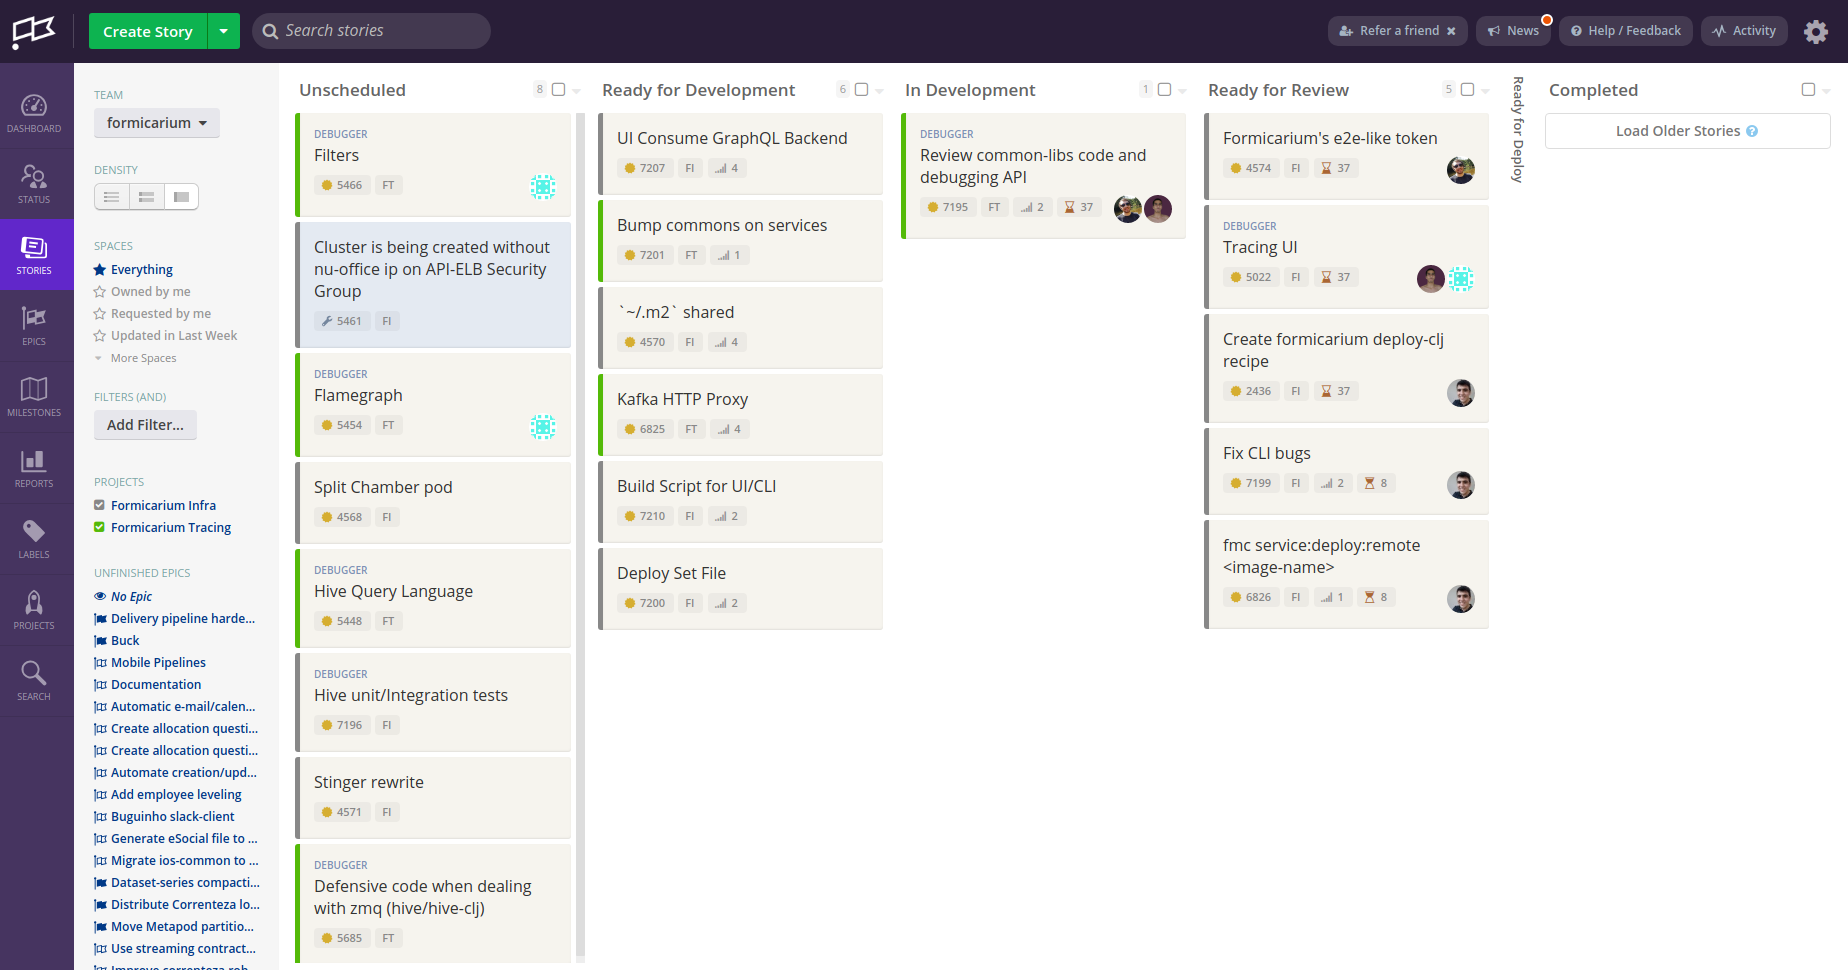
\includegraphics[scale=0.20]{pictures/clubhouse-fmc.png}
                \end{center}
                \label{fig:clubhouse}
                \legend{Fonte: os autores - 2018-11-10}
            \end{figure}

        \subsection{Slack}
            Slack \cite{slack} \textit{software} para equipes que proporciona mensageria instantânea, canais de conversa, \textit{workspaces} e muitas integrações (por exemplo, utilizamos a do \textit{GitHub} para acompanhar os nossos repositórios).
    

\chapter{Especificação de Requisitos do Sistema}
    Escolhemos especificar os requisitos de sistema do nosso projeto seguindo o modelo de referência ODP, pois ele apresenta uma forma de simplificar a descrição de sistemas complexos por meio dos seus Pontos de Vista.\cite{odppart1} Sabíamos também que gostaríamos se seguir alguns princípios de projeto, descritos na Tabela \ref{principios_de_projeto}. Esses princípios foram resultado de conversas com engenheiros de software e interessados no projeto, e nos ajudaram a guiar durante a definição dos requisitos de sistema.
    \begin{table}
        \centering
        \caption{Princípios de Projeto}
        \label{principios_de_projeto}
        \resizebox{\textwidth}{!}{%
        \begin{tabular}{|l|p{10cm}|}
            \hline
            Princípio de Projeto                 & Descrição \\ \hline
            Ambientes de curta duração           & O desenvolvedor deve ser capaz de criar e deletar ambientes com rapidez e facilidade                                 \\ \hline
            Visualização de fluxos complexos     & O desenvolvedor deve ser capaz de visualizar o resultado de suas requisições HTTP e mensagens Kafka                  \\ \hline
            Ambiente parecido com o local        & O desenvolvedor deve ter uma experiência de desenvolvimento similar com o ambiente de sua máquina                    \\ \hline
            Esconde complexidade de configuração & O desenvolvedor não deve precisar conhecer a configuração dos serviços que ele precisa disponíveis no ambiente dele. \\ \hline
        \end{tabular}
        }
        \legend{Fonte: os autores}
    \end{table}
	\section{Ponto de Vista da Empresa}
	    As empresas que podem se beneficiar do nosso projeto devem ter alguma semelhança com o processo de negócio de desenvolvimento e entrega de novas funcionalidades, descritos respectivamente nas Figuras \ref{fig:build-ci} e \ref{fig:automated-deploy}. O primeiro processo descreve como uma alteração de código por um desenvolvedor gera novas imagens Docker, que são guardadas em um catálogo chamado \textit{Docker Registry}. Exemplos de \textit{Docker Registry} são o DockerHub e o Quay.io. Já o segundo processo, descreve como uma imagem desses catálogo é implantada de forma automatizada pelo Servidor de Entrega Contínua.
	    \begin{figure}[htb]
    	    \centering
    	    \caption{Processo de Entrega Contínua - Construção da imagem Docker}
    	    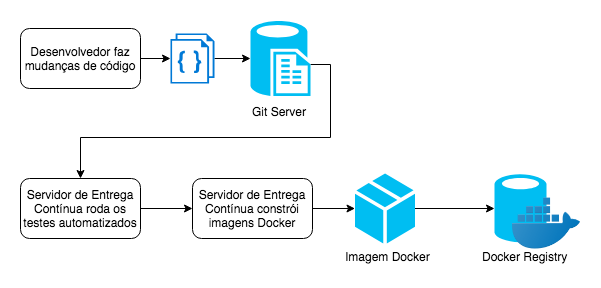
\includegraphics[scale=0.7]{pictures/especificacao-de-requisitos/build-ci.png}
    	    \legend{Fonte: os autores}
    	    \label{fig:build-ci}
	    \end{figure}
	    \begin{figure}[htb]
    	    \centering
    	    \caption{Processo de Entrega Contínua - Implantação automatizada}
    	    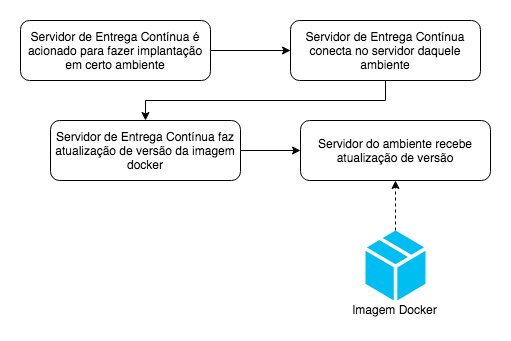
\includegraphics[scale=0.7]{pictures/especificacao-de-requisitos/automated-deploy.png}
    	    \legend{Fonte: os autores}
    	    \label{fig:automated-deploy}
	    \end{figure}
	\section{Ponto de Vista da Informação}
	    O objetivo dessa seção é apresentar a organização das informações por todos os componentes do sistema. A Figura \ref{fig:info-contexts} representa os três principais contextos onde as informações são modeladas, e como é o fluxo de informações. 
	    \begin{figure}[htb]
    	    \centering
    	    \caption{Contextos de informação e seu fluxo}
    	    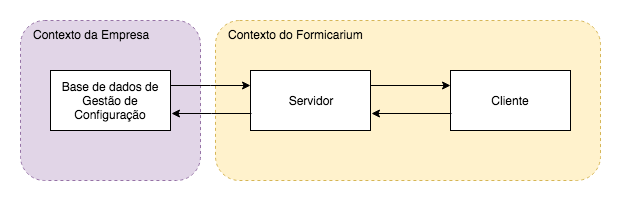
\includegraphics[scale=0.67]{pictures/especificacao-de-requisitos/information-contexts.png}
    	    \legend{Fonte: os autores}
    	    \label{fig:info-contexts}
	    \end{figure}
	    \subsection{Contexto da Empresa}
	        O contexto da empresa refere-se a uma base de dados pré-existente capaz de fornecer as configurações de uma aplicação dado o ambiente: teste, homologação e produção, tradicionalmente. Assim, a modelagem dessa base de dados pode ser arbitrária em relação ao sistema do Formicarium.
	    \subsection{Contexto do Formicarium}
	        \subsubsection{Servidor}
	        A Figura \ref{fig:info-server} representa a modelagem da configuração necessária para rodarmos uma aplicação. Note que uma aplicação pode possuir múltiplas interfaces e pode constituir por múltiplos contêineres. Isso permite maior flexibilidade na implantação e modelagem de aplicações.
	        \begin{figure}[htb]
        	    \centering
        	    \caption{Modelagem das Informações no Servidor}
        	    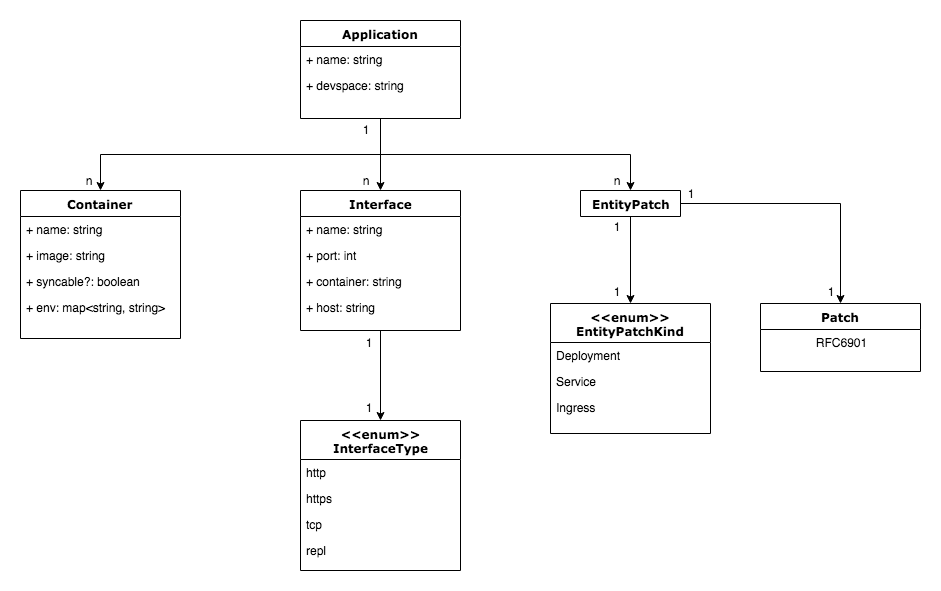
\includegraphics[scale=0.40]{pictures/especificacao-de-requisitos/info-server.png}
        	    \legend{Fonte: os autores}
        	    \label{fig:info-server}
	        \end{figure}
	        \subsubsection{Cliente}
	            
	\section{Ponto de Vista da Computação}
	    O Ponto de Vista da computação está diretamente ligado a distribuição. Não diz respeito aos mecanismos de interação, mas decompõe o sistem em objetos capazes de realizar funções e interagir por interfaces bem definidas \cite{odppart1}.
	    \subsection{Arquitetura de Referência} %% TODO: Leal
	        A arquitetura deste projeto compartilha conceitos e mecanismos com arquiteturas de Plataformas como Serviço (\textit{Platform as a Service}), em particular a arquitetura do Heroku.
	        
	        O Heroku se descreve da seguinte forma: "Heroku é uma plataforma de nuvem baseada em um sistema de contêineres gerenciado, com integração a serviços de dados e um poderoso ecossistema, para implantação e execução de aplicações modernas. O \textit{Heroku Developer Experience} é uma abordagem centrada na aplicação para entrega de software, integrada com as mais populares ferramentas e fluxos de trabalhos atuais." (\citeauthor{herokuplatform}, \citeyear{herokuplatform}).
	        
	\section{Ponto de Vista da Engenharia}
	\section{Ponto de Vista da Tecnologia}


\chapter{Projeto e Implementação}
    \section{Devspaces}
    
    Um Devspace, como foi batizado pelo grupo, é um ambiente de desenvolvimento isolado que roda em cima da plataforma Formicarium. Ele é o ambiente que o desenvolvedor vai ter disponível para uso e que vai interagir durante o seu tempo testando e desenvolvendo os serviços. 
    
    Os Devspaces são provisionados e configurados de forma automática pelo serviço Soil, a medida que um desenvolvedor requisita sua criação através da CLI. Para obter dados de configuração e setup inicial do Devspace, o Soil consulta um servidor de configurações via Webhooks, esse encarregado de fornecer todo configuração específica da empresa para fazer o bootstrap de um novo Devspace.
    
    Objetivamente, os Devspaces são Namespaces do Kubernetes que são gerenciados pelo Soil, além dos recursos padrões do Kubernetes, esse Namespaces acabam recebendo serviços adicionais do Formicarium, sendo esses o Hive e o Tanajura. A interação com os Devspaces é feito sempre através da CLI do Formicarium, não exigindo que o usuário tenha que ter o ferramental do Kubernetes instalado e configurado em sua máquina.
    
    Dentro de um Devspace os serviços que rodam nele conseguem se localizar entre si por meio do servidor de DNS do Kubernetes que garante isolamento entre Namespaces, dessa forma conseguimos alcançar um isolamento entre serviços entre Devspaces, mesmo que 2 desenvolvedores estejam executando o mesmo serviço. Além disso, cada Devspace recebe do Config Server um conjunto de aplicações de infra-estrutura ou de uso comum, que também garante isolamento dos demais Devspaces, como por exemplo, a existência de um broker de mensageria por Devspace. não havendo confusão na produção e consumo de mensagens.
    
        \begin{figure}[htbp]
			\caption{\label{fig_devspace1}Anatomia de um Devspace}
			\begin{center}
			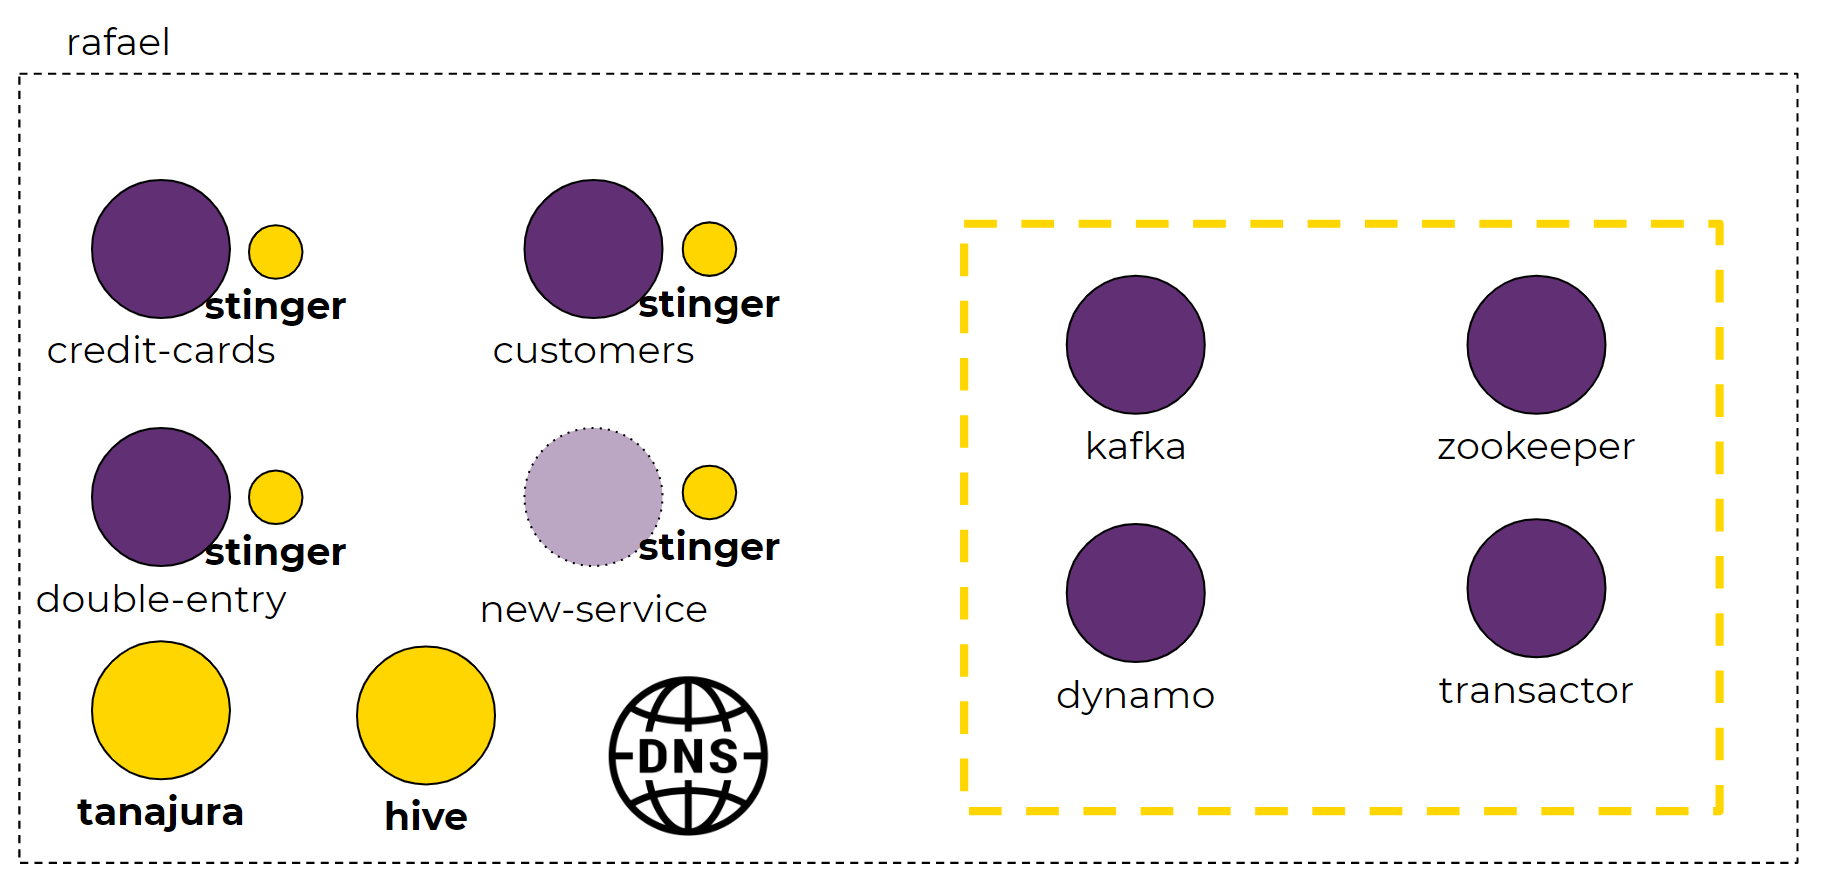
\includegraphics[scale=0.30]{pictures/devspace1.png}
			\end{center}
			\legend{Fonte: os autores}
			% \caption{Fonte: própria}
		\end{figure}
    
    	\begin{figure}[htbp]
			\caption{\label{fig_create_devspace}Fluxo de Criação de Devspaces}
			\begin{center}
			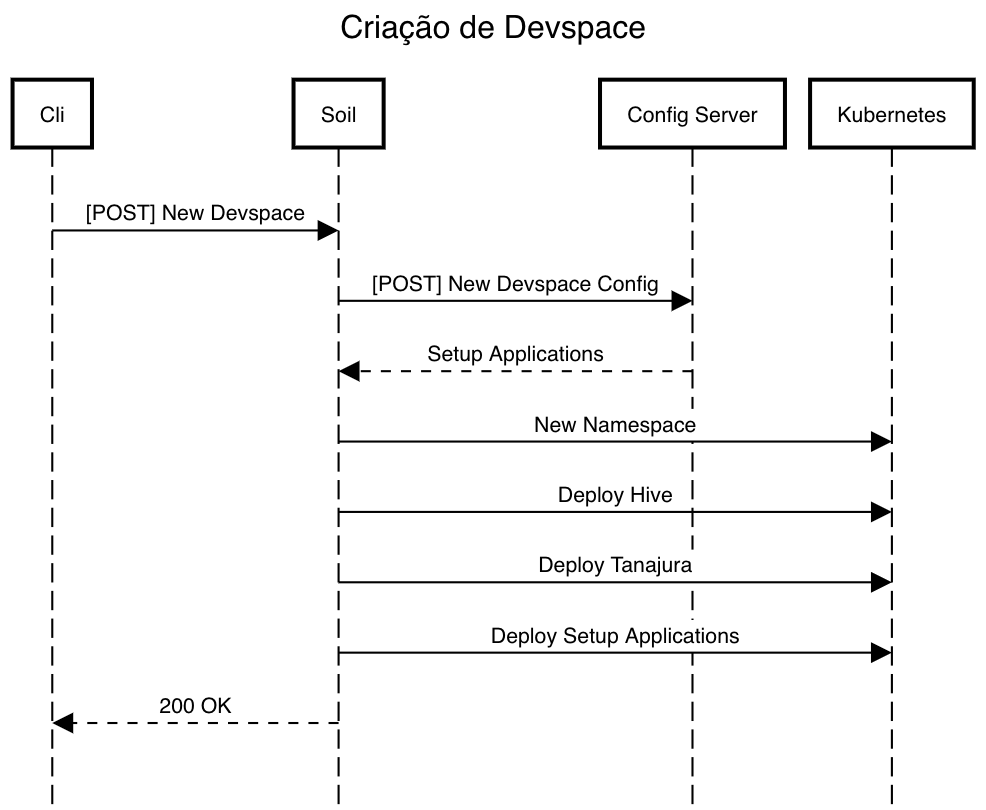
\includegraphics[scale=0.40]{pictures/create-devspace.png}
			\end{center}
			\legend{Fonte: os autores}
			% \caption{Fonte: própria}
		\end{figure}

	\section{FileSync}

	Um dos grandes desafios do projeto foi a construção de um sistema para sincronização de arquivos em uma arquitetura distribuída de microsserviços.
	
	O caso de uso principal para esta funcionalidade é permitir que o engenheiro da Nubank pudesse iterar de maneira mais rápida no desenvolvimento de um novo microsserviço ou em modificações de algum existente.
	
	Do ponto de vista da empresa, esta era um dos requisitos mais desejados e que mais agregaria valor ao produto final, dado que é uma ferramenta extremamente poderosa para o engenheiro, garantindo-lhe mais produtividade e liberdade enquanto estivesse desenvolvendo.
	
	Este sistema de sincronização de arquivos precisava atender algumas premissas:
	- Deve se integrar facilmente ao workflow do engenheiro, para haver um incentivo à sua adoção.
	- Segurança: Os arquivos trafegados não devem ser, de maneira alguma, expostos para a internet ou suscetíveis a ataques como Man in the middle, dado que o conteúdo trafegado é extremamente sensível (códigos fonte dos produtos da empresa)
	- Velocidade: Quanto mais rápido for o processo de sincronização, mais dinâmico será o processo, permitindo iterações mais rápidas e, consequentemente, maior produtividade.

	Para entender o problema que o sistema de Filesync se propõe a resolver, é preciso entender o cenário:
	
	Os serviços em que o engenheiro está trabalhando não estão sendo compilados e executados na mesma máquina em que está o código fonte. Na verdade eles estão sendo executados em um contêiner Docker, gerenciado por um \textit{cluster} Kubernetes, operando em uma infraestrutura de \textit{hardware} fornecida pela AWS EC2. Para que mudanças no código fonte fossem de fato percebidas pelo desenvolvedor, este precisaria compilar uma nova imagem Docker com o código fonte atualizado, publica-lá em um repositório de contêineres e realizar a implantação desta nova imagem no \textit{cluster} remoto. Este processo, em um contexto de desenvolvimento, é extremamente ineficiente, o que tornaria a ferramenta pouco dinâmica e não atrativa para o engenheiro.

	Para evitar a geração de uma nova imagem Docker a cada iteração no código fonte, foi desenvolvida uma imagem genérica capaz de compilar e executar qualquer serviço da Nubank em modo de desenvolvimento. Esta imagem foi apelidada de Chamber e uma de suas características é a sua extensibilidade, permitindo que em melhorias futuras sejam desenvolvidas versões para outras linguagens e plataformas (Como por exemplo \textit{Node.js}, \textit{Ruby}, \textit{Scala}, \textit{etc.}). Para implantação no Nubank, foi desenvolvida a imagem Chamber-lein, capaz de executar programas escritos em \textit{Clojure}, principal linguagem utilizada nos microsserviços do Nubank.
	
	Além disto, esta imagem tem um componente de software capaz de atualizar o código do serviço que está sendo executado dentro do contêiner através do Git.
	
% 	\section{Arquitetura da solução}
% 		\begin{figure}[htb]
% 			\caption{\label{fig_arquitetura1}Arquitetura da solução}
% 			\begin{center}
% 			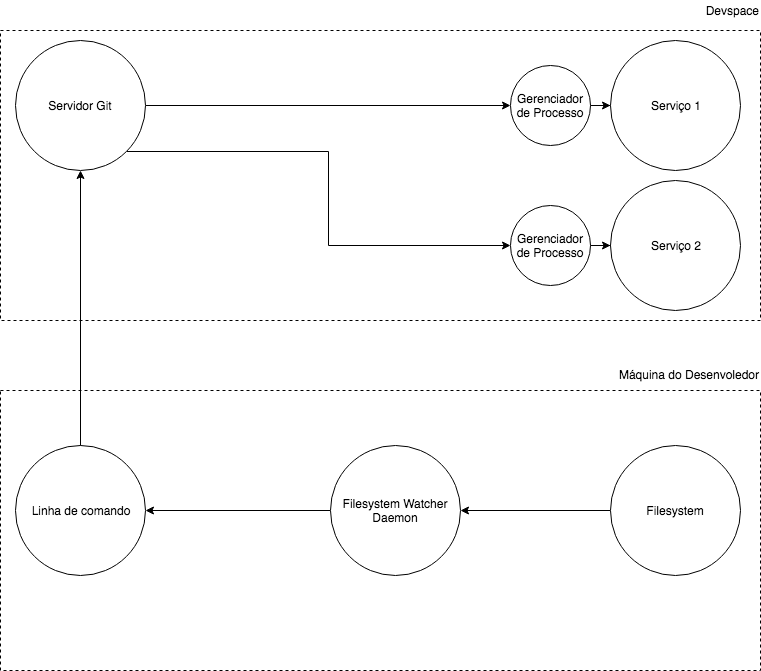
\includegraphics[scale=0.50]{pictures/arquitetura-da-solucao.png}
% 			\end{center}
% 			\legend{Fonte: os autores}
% 		\end{figure}
	
	\subsection{Servidor web para Git (Tanajura)}
	Um dos componentes do sistema de sincronização de arquivos é um servidor web apelidado de \textit{Tanajura}. O serviço tem como principal responsabilidade ser um \textit{hub} de repositórios Git.
	
	Nestes repositórios está o código fonte dos serviços em que o desenvolvedor está trabalhando no momento e o Git é utilizado como mecanismo de sincronização entre o sistema de arquivos local da máquina do desenvolvedor e o sistema de arquivos do contêiner em que está sendo executado a aplicação, em um \textit{cluster} Kubernetes remoto.
	
	O serviço conta com \textit{endpoints} para gerenciamento de repositórios (operações de criação, remoção e consulta) através de uma interface REST, bem como um \textit{endpoint} que implementa os protocolos do Git para transferência e dados através de HTTP. Assim é possível para qualquer cliente Git a realização das operações básicas como \textit{push}, \textit{pull} e \textit{fetch}.
	
	Os repositórios Git neste serviço têm como característica a efemeridade, ou seja, eles não precisam ser de mecanismos robustos de persistência e só existem para fins de sincronização entre dois sistemas de arquivos, podendo ser sobrescritos e apagados a qualquer momento sem perda de dados importantes.
	
	A escolha do Git para este sistema de sincronização pode ser justificado por algumas de suas características que atendiam os requisitos definidos:
	
	- O binário do Git já está presente na máquina do desenvolvedor do Nubank, pois todos trabalham com Git em seu dia-a-dia.
	
	- É um método eficiente para troca de dados, pois os \textit{commits} são criados a partir das modificações feitas em arquivos, ou seja, apenas as diferenças são transmitidas pela rede.
	
	- A troca de dados pode ser criptografada com SSL.

	Ao receber um \textit{push} em algum repositório Git, o \textit{Tanajura} identifica qual o serviço associado ao repositório e faz uma requisição HTTP para o \textit{Soil} a fim de obter a URL do Gerenciador de Processo (\textit{Stinger}) deste serviço.
	
	Uma vez obtida esta URL, o serviço \textit{Tanajura} faz uma requisição para o \textit{Stinger} avisando-o de que há uma nova versão do código disponível para ser sincronizada.
	
	Este, por sua vez, realiza um \textit{pull} no repositório remoto para obtenção do código atualizado e, após o recebimento dos arquivos, executa os \textit{scripts} necessários para recompilação e execução do código.
	
	Esta parte do processo pode ser representada pelo seguinte diagrama de sequência:
		\begin{figure}[htb]
			\caption{\label{fig_arquitetura2}Fluxo do Tanajura}
			\begin{center}
			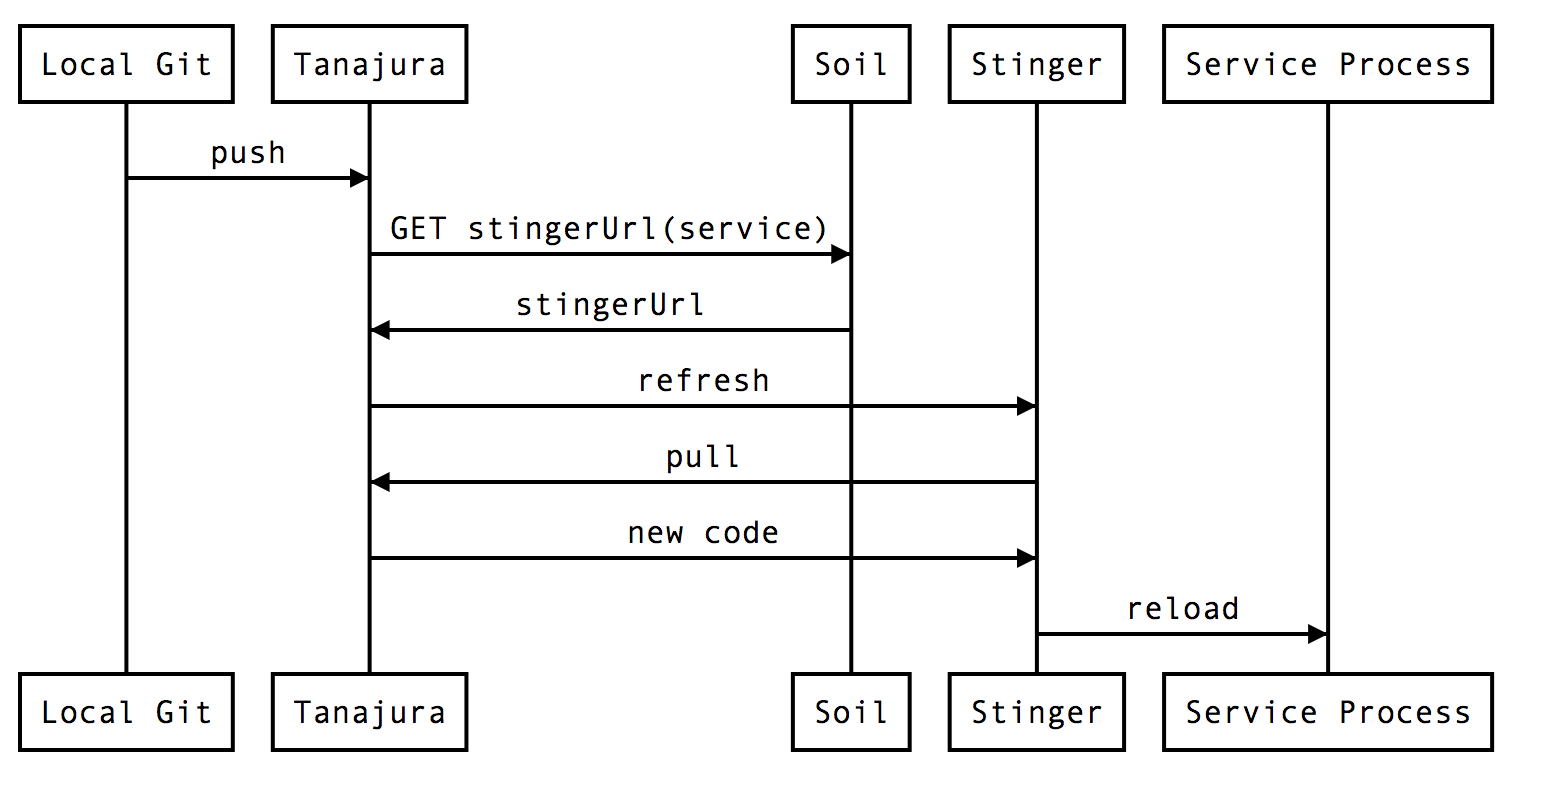
\includegraphics[scale=0.29]{pictures/tanajura-flow.png}
			\end{center}
			\legend{Fonte: os autores}
			% \caption{Fonte: própria}
		\end{figure}

	Em termos práticos, o processo ocorre da seguinte maneira:
	
	Quando o desenvolvedor deseja implantar em seu devspace um serviço com capacidades de sincronização, ele digita o seguinte o comando:

	\begin{verbatim}
	fmc service:deploy:local my-service -f ./config.json /path/to/service
	\end{verbatim}

	Este comando irá realizar a implantação de um serviço chamado \textit{"my-service"}, utilizando o arquivo de configuração \textit{"./config.json"} a partir da pasta local \textit{"/path/to/service"}

	\subsection{Gerenciador de Processos (Stinger)}	
	
	Para que fosse possível o método de sincronização de arquivos utilizando Git foi necessário o desenvolvimento de uma aplicação que, através de uma interface HTTP exposta para o \textit{cluster}, pudesse fazer \textit{pull} em um repositório Git remoto para obtenção do código fonte atualizado e, após o recebimento dos arquivos, fosse possível executar um comando arbitrário para que o processo do serviço pudesse ser recarregado.
	
	Esta aplicação foi apelidada de Stinger e é o binário executado primariamente pela imagem Docker onde os serviços são executados (esta imagem será descrita em detalhes mais adiante). Os endpoints HTTP disponíveis neste serviço são:

    \textbf{POST /reset}
	\newline
	Ao receber uma requisição neste endpoint, o Stinger termina o processo do serviço em execução através de seu identificador de processo (\textit{process ID}) e executa o \textit{script} de \textit{cleanup}. Após a garantia de que o processo do serviço foi terminado com êxito, é executado o \textit{script} de \textit{start}, que garante sua reinicialização.
	
	\textbf{POST /pull}
	\newline
	Ao receber uma requisição neste endpoint, o Stinger executa o comando git pull origin master para obter a versão mais recente do código no repositório remoto. É possível, através de parâmetros no corpo da requisição, fazer com que o processo do serviço seja reinicializado logo após o recebimento do código atualizado.

	Quando o Stinger é iniciado, ele verifica a existência do repositório Git local e, caso não o encontre, executa o comando \textit{git clone [url do repositório] [pasta local]} para obter a versão inicial do código. Logo após o recebimento dos arquivos, é feito o processo de inicialização do serviço.

	É possível configurar diversos parâmetros de funcionamento do \textit{Stinger} através de variáveis de ambiente. Os mais relevantes são:
	
	\textbf{APP\_PATH}
	\newline
	É a o caminho para o diretório local onde o Stinger irá clonar o código do repositório remoto.
	
	\textit{exemplo: /app}

	\textbf{STINGER\_SCRIPTS}
	\newline
	Caminho para o diretório local onde o Stinger irá executar os scripts para gerenciar os ciclos de vida do serviço. Dentro desta pasta, devem estar presentes os scripts de start e cleanup.
	
	\textit{exemplo: /scripts}
	
	\textbf{GIT\_URL}
	\newline
	É a URL de onde o \textit{Stinger} fará o \textit{git clone} inicial dos arquivos.
	
	\textit{exemplo: \url{https://tanajura.joe.formicarium.nubank.com.br/service-name}}
	
	\textbf{START\_AFTER\_PULL}
	\newline
	Caso esta variável esteja setada, o \textit{Stinger} irá reinicializar o processo sempre após o recebimento de novo código através do \textit{pull}. Esta configuração existe porque em certas linguagens de programação (como a utilizada pela Nubank) não é necessário recompilar e nem executar nenhum comando para que o novo código obtido seja aplicado no processo em execução.
    
	De maneira geral, o \textit{Stinger} é um gerenciador de processos integrado com o Git e que expõe suas funcionalidades através de um servidor HTTP.

\section{Frontend}  
    \subsection{Organização do código}
        Para oferecer uma interface amigável aos usuários, foram construídas duas aplicações: uma Interface de linha de comando e uma Aplicação \textit{Desktop}. Ambas têm funcionalidades semelhantes, porém a segunda oferece elementos de interface gráfica essenciais para a construção do módulo de \textit{Distributed Debugger} do sistema.

        Como as duas aplicações compartilham diversos módulos, todo o código comum foi extraído para uma biblioteca (chamada \textit{common}) e seu código fica disponível para ambas as aplicações através de um sistema de dependências oferecido pelo NPM.

        Foi tomado o cuidado de não se criar acoplamentos dos módulos desta biblioteca com casos de uso específicos de cada aplicação, tornando o código mais reaproveitável e desacoplado, com responsabilidades bem definidas.

        O código dos três módulos vive em mesmo repositório Git, dividido apenas por pastas. Esta prática é comum para o gerenciamento de múltiplos módulos que compõe um sistema maior e  repositórios com esta característica são denominados \textit{monorepos}.

        Este tipo de organização é vantajosa pois preserva os benefícios de desacoplamento das diferentes partes do sistema, porém eliminando, através do uso de ferramentas específicas, as complexidades de se gerenciar as dependências entre os diversos módulos, tanto no estágio de desenvolvimento quanto nos estágios de compilação e publicação.

        Para gerenciar as dependências do \textit{monorepo}, foi utilizado a ferramenta \textit{yarn workspaces}, que otimiza o uso de memória em disco do código fonte e o tempo de instalação inicial para novos desenvolvedores através do compartilhamento das dependências comuns entre os vários módulos. Ela também é responsável por criar \textit{links} simbólicos (\textit{symlinks}) entre os módulos quando em estágio de desenvolvimento. Os \textit{symlinks} permitem iterações mais rápidas de desenvolvimento, pois uma mudança no código de uma dependência irá refletir automaticamente nos módulos dependentes, sem a necessidade de se incrementar versões e recompilar partes do programa.

        Todos os módulos do projeto utilizam \textit{Semantic Versioning} como padrão versionamento. O incremento é feito automaticamente através de uma ferramenta que analisa as mensagens presentes nos commits do Git para determinar, através de \textit{tokens} pré-definidos, qual será o incremento de versão: \textit{Major}, \textit{minor}, \textit{patch}.

        Além do incremento automático em cada módulo, foi utilizada a ferramenta \textit{Lerna} para determinar quais módulos e dependências devem ter suas versões atualizadas, através também da análise de quais arquivos foram modificados nos commits desde a última atualização.

        Todo este ferramental tornou a experiência de desenvolvimento deste projeto muito mais eficiente e facilitará também sua manutenção.

    \subsection{Interface de linha de comando}
        
        Para a construção deste software, foi utilizado a linguagem Typescript, com a plataforma Node.js. A framework para desenvolvimento foi a ocli, mantida pela Salesforce.
        
        Este software é distribuído através do NPM (\textit{Node Package Manager)}. Por ser uma ferramenta já presente nos computadores dos engenheiros do Nubank, a instalação da linha de comando se torna simples e rápida, basta executar o comando
    \begin{verbatim}
	    npm install -g @formicarium/cli
	\end{verbatim}
	
	Com isso, o binário \textit{fmc} já fica disponível para ser executado através do terminal.
	
	Para atualizar a versão do software após a publicação de alguma modificação, basta o comando
	\begin{verbatim}
	    npm update -g @formicarium/cli
	\end{verbatim}
	
	Este mecanismo de fácil distribuição e atualização foi escolhido para facilitar ainda mais a adesão dos engenheiros ao uso do ecossistema Formicarium.

    A interface de linha de comando apresenta suas funcionalidades divididas em subprogramas, cada um referente a um conjunto de casos de uso agrupados logicamente. Utilizando o comando \textit{help}, o engenheiro tem acesso à documentação da ferramenta, podendo listar os subprogramas e comandos disponíveis dentro de cada nível hierárquico de funcionalidades e entender o que fazem através de descrições e exemplos de uso.

    Por exemplo, ao requisitar ajuda no contexto geral da linha de comando:

    \begin{verbatim}
    A CLI to operate on Formicarium
    VERSION
        @formicarium/cli/1.3.2 darwin-x64 node-v11.1.0
    USAGE
        $ fmc [COMMAND]
    COMMANDS
        devspace  Creates a Devspace
        git       Configures local fmcgit and hive
        help      display help for fmc
        repl      Connects to remote repl. If no service is provided, connects on Hive's Repl
        service   Deletes a service in the current Devspace
        setup     Configures Formicarium CLI to one cluster
    \end{verbatim}
    
    Ao requisitar ajuda para um contexto específico (no caso, o contexto \textit{devspace}):
    \begin{verbatim}
    Creates a Devspace
    
    USAGE
      $ fmc devspace:COMMAND
    
    COMMANDS
      devspace:create    Creates a Devspace
      devspace:delete    Deletes a Devspace
      devspace:info      Get information for the current devspace
      devspace:list      List availables Devspaces
      devspace:services  Lists the services in your devspace
      devspace:use       Configures to use one Devspace context
    \end{verbatim}
    
    
    Ao requisitar ajuda para um comando específico (no caso, o comando \textit{devspace:create}):
    \begin{verbatim}
    Creates a Devspace
    
    USAGE
      $ fmc devspace:create ID
    
    OPTIONS
      -h, --help  show CLI help
      --test
    
    EXAMPLE
      $ fmc devspace:create paps
    \end{verbatim}


    A facilidade proporcionada ao engenheiro do Nubank para entender o uso da ferramenta através desta documentação interativa fez parte da estratégia do grupo para disseminação e adesão da ferramenta por toda a empresa de maneira escalável.


    
    \begin{table}[ht]
    \centering
    \begin{tabular}{l l}
    Comando & Descrição \\
    \hline
      devspace:create    & Cria um novo devspace \\
      devspace:delete    & Deleta um devspace existente \\
      devspace:info      & Obtém informações sobre o devspace atual \\
      devspace:list      & Lista todos os devspaces disponíveis \\
      devspace:services  & Lista todos os serviços em execução no devspace atual \\
      devspace:use       & Muda o contexto do Formicarium para utilizar outro devspace \\
      sync:push          & Sincroniza o sistema de arquivos local com o de um serviço remoto \\
      service:delete     & Deleta uma serviço em execução no devspace atual \\
      service:deploy     & Implanta um novo serviço no devspace atual \\
      service:logs       & Obtém os \textit{logs} de um serviço \\
      service:restart    & Reinicia o processo do serviço \\
      repl               & Inicia uma sessão de REPL com o serviço \\
    \end{tabular}
    \caption{Comandos disponíveis e uma breve descrição do que fazem}
    \label{tab:roles}
    \end{table}

    \subsection{Aplicação \textit{Desktop}}

    Como parte do ferramental do ambiente Formicarium, foi desenvolvida uma aplicação Desktop multiplataforma (Windows, Linux, OS X) com o intuito de melhorar a experiência dos usuários nas funções mais comuns e também para atender requisitos do sistema que exigiam interfaces gráficas mais interativas e avançadas. A aplicação foi desenvolvida utilizando tecnologias web (HTML5, CSS3 e Javascript), o que tornou possível sua execução em diferentes plataformas utilizadas pelos engenheiros do Nubank. Como era necessário o uso de \textit{APIs} nativas do sistema (como acesso ao sistema de arquivos e execução de outros programas a partir da interface gráfica) que não seriam possível no browser, foi utilizada a \textit{framework} Electron para empacotar a aplicação em um binário capaz de ter acesso às \textit{system calls} necessárias. Electron é a framework por trás de diversos projetos populares como Slack, WhatsApp Desktop, Visual Studio Code, Atom, Spotify entre outros. Além disso, conta com uma enorme comunidade, melhorando ainda as características de manutenibilidade de software da solução.

    Para a sua distribuição dentro do Nubank, o software compilado foi disponibilizado em um \textit{bucket} da \textit{AWS S3} acessível apenas para funcionários credenciados \textit{download} e execução para começar a utilizá-lo.

    A aplicação ainda não conta com sistemas automatizados de atualização, sendo necessária a obtenção manual de uma nova versão sempre que o engenheiro veja a necessidade de atualização. Este mecanismo de atualização poderá ser aprimorado em melhoria futuras.

    \subsection{Gerenciamento de Devspaces}
    Esta área tem como objetivo mostrar ao engenheiro os Devspaces disponíveis para serem utilizados. Normalmente o Devspace pessoal do engenheiro estará selecionado, porém é possível por exemplo alternar entre este e o Devspace do \textit{squad} ou ainda o de algum colega caso queiram compartilhar alguma configuração para reproduzir ambientes de testes e desenvolvimento.

    \begin{figure}[htb]
    	\caption{\label{fig_frontend_devspaces}Tela Lista de Devspaces}
    	\begin{center}
    	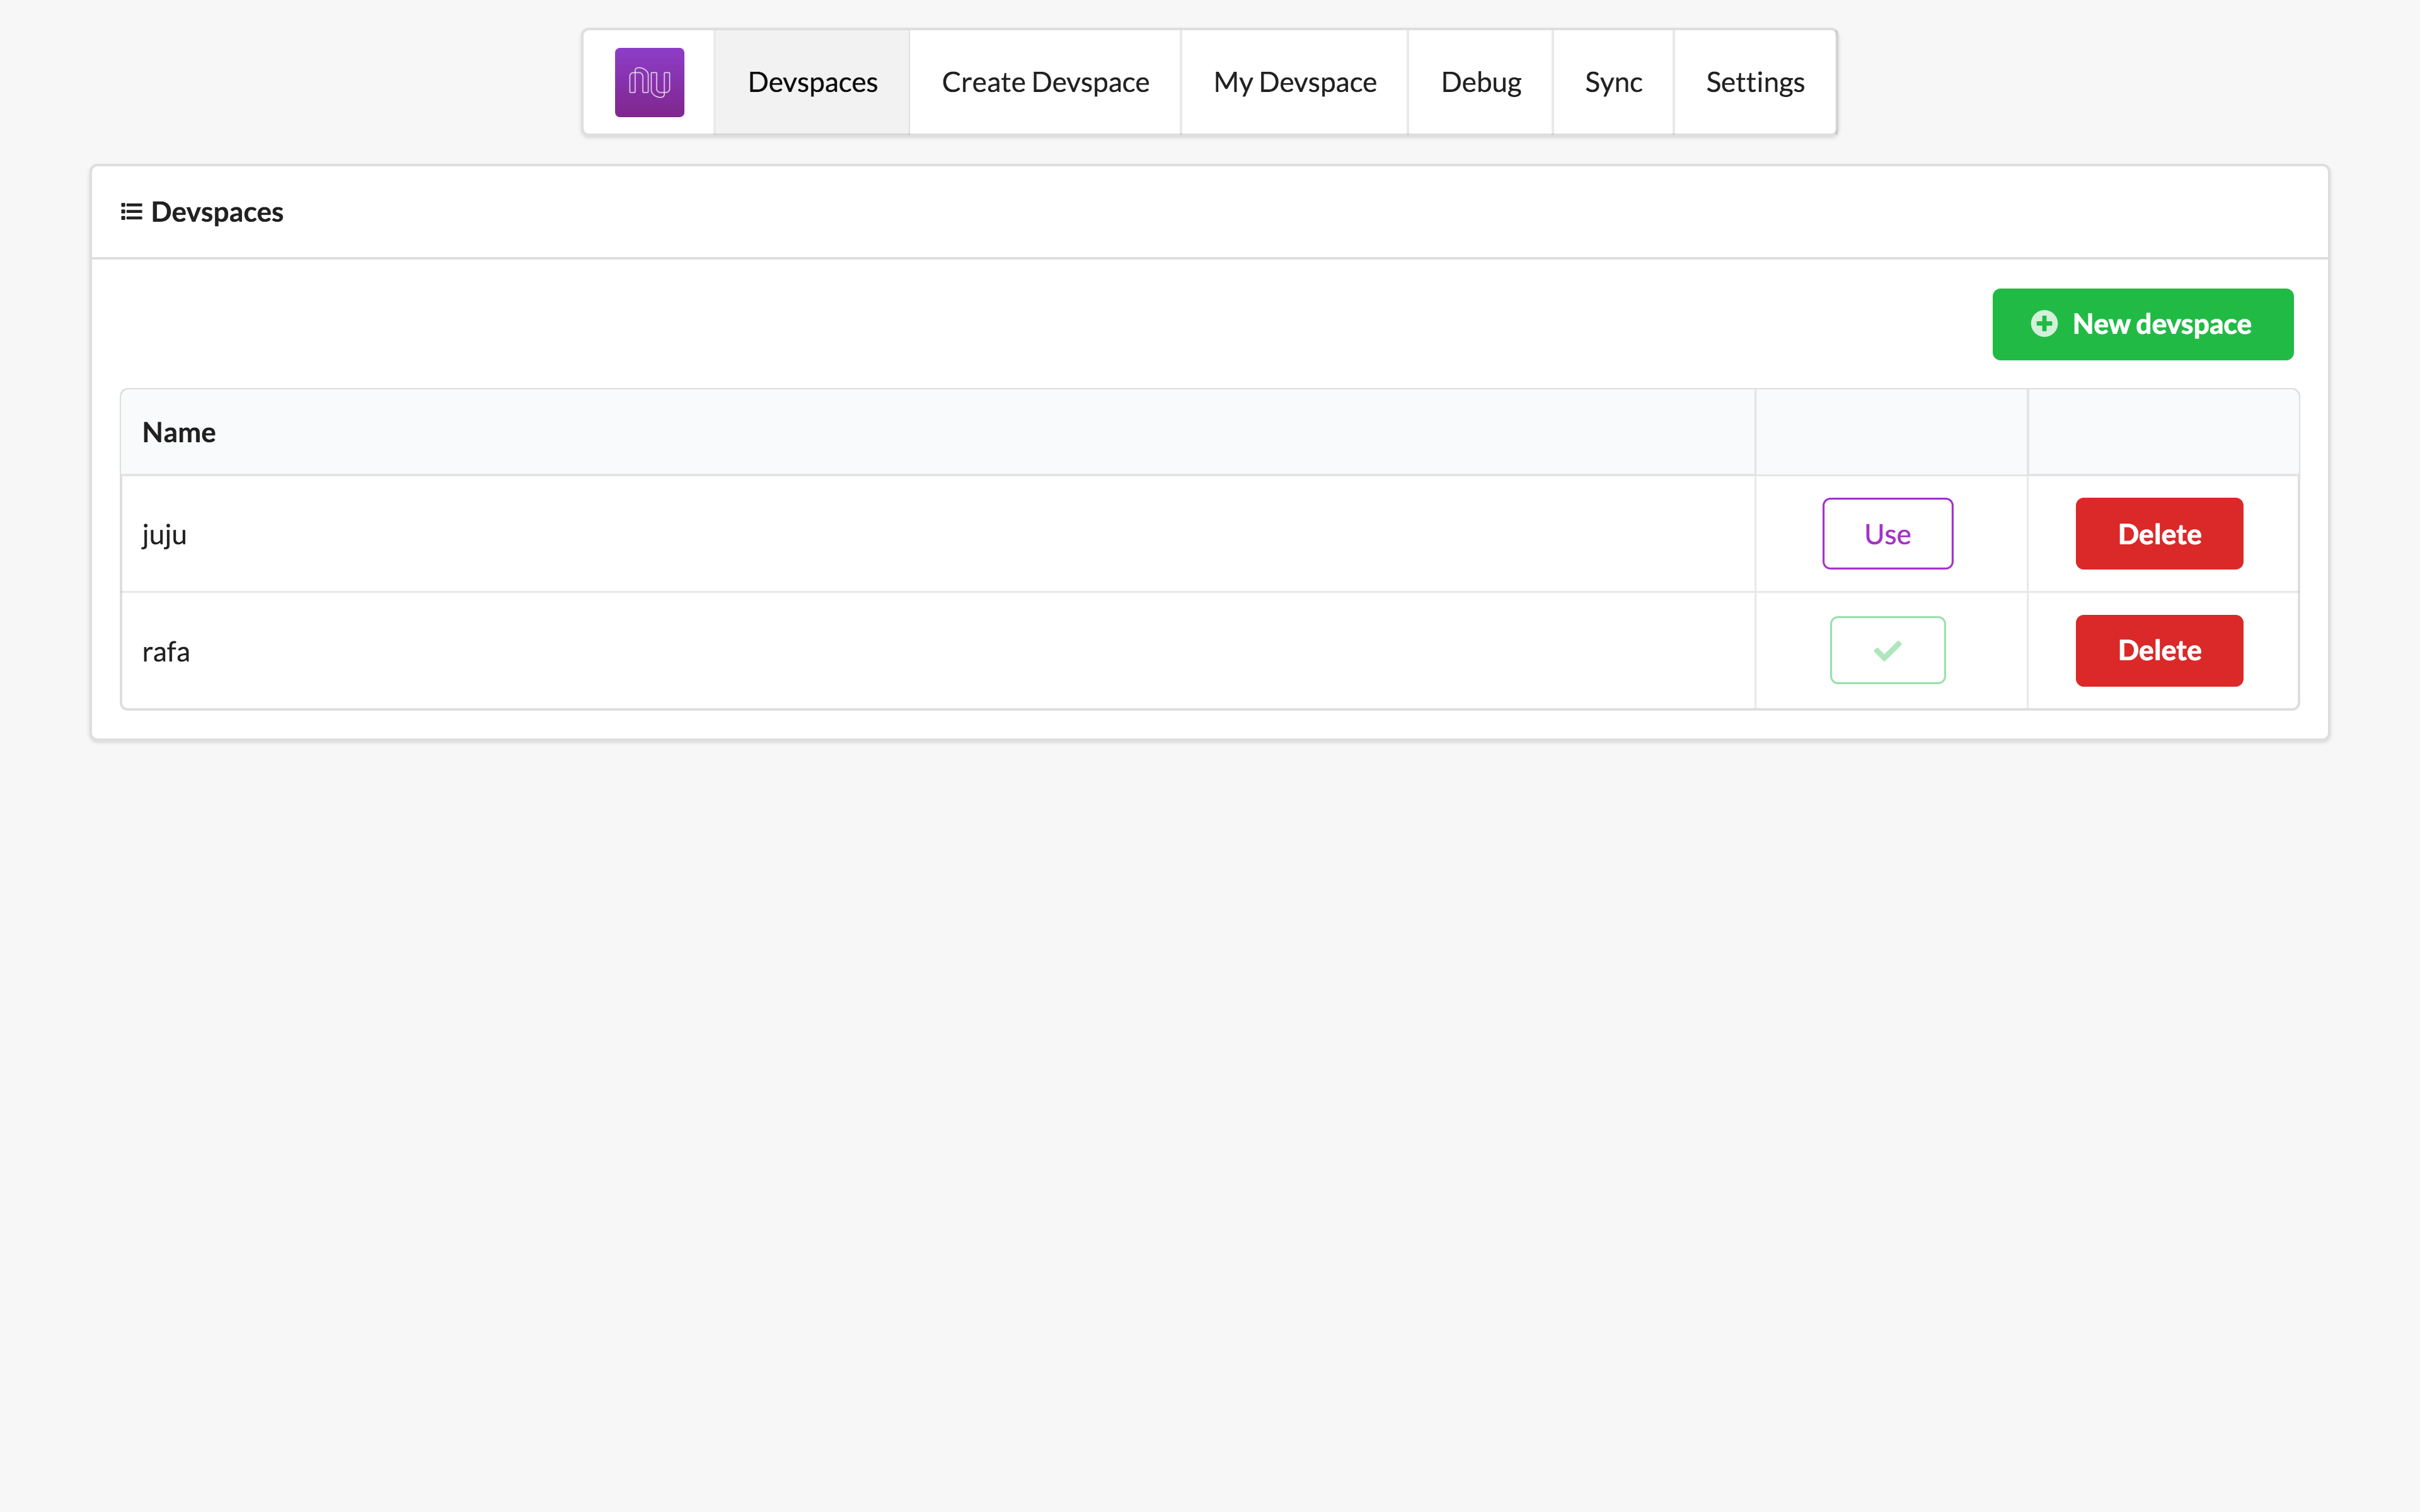
\includegraphics[width=\textwidth,keepaspectratio]{pictures/frontend/frontend-devspaces.png}
    	\end{center}
    	\legend{Fonte: Elaborado pelos autores}
    \end{figure}



    \subsection{Devspace}
    Esta área tem como objetivo mostrar informações e proporcionar interações com o Devspace específico selecionado pelo engenheiro.

    \subsubsection{Infraestrutura}
    Nesta área o engenheiro pode conferir o status dos serviços básicos de infraestrutura do Devspace, como o Hive (para \textit{Distributed Tracing}) e o Tanajura (para sincronização de arquivos). Também é possível extrair os logs destes serviços em tempo real.

    \begin{figure}[htb]
    	\caption{\label{fig_frontend_devspace_info}Tela Informações do Devspace}
    	\begin{center}
    	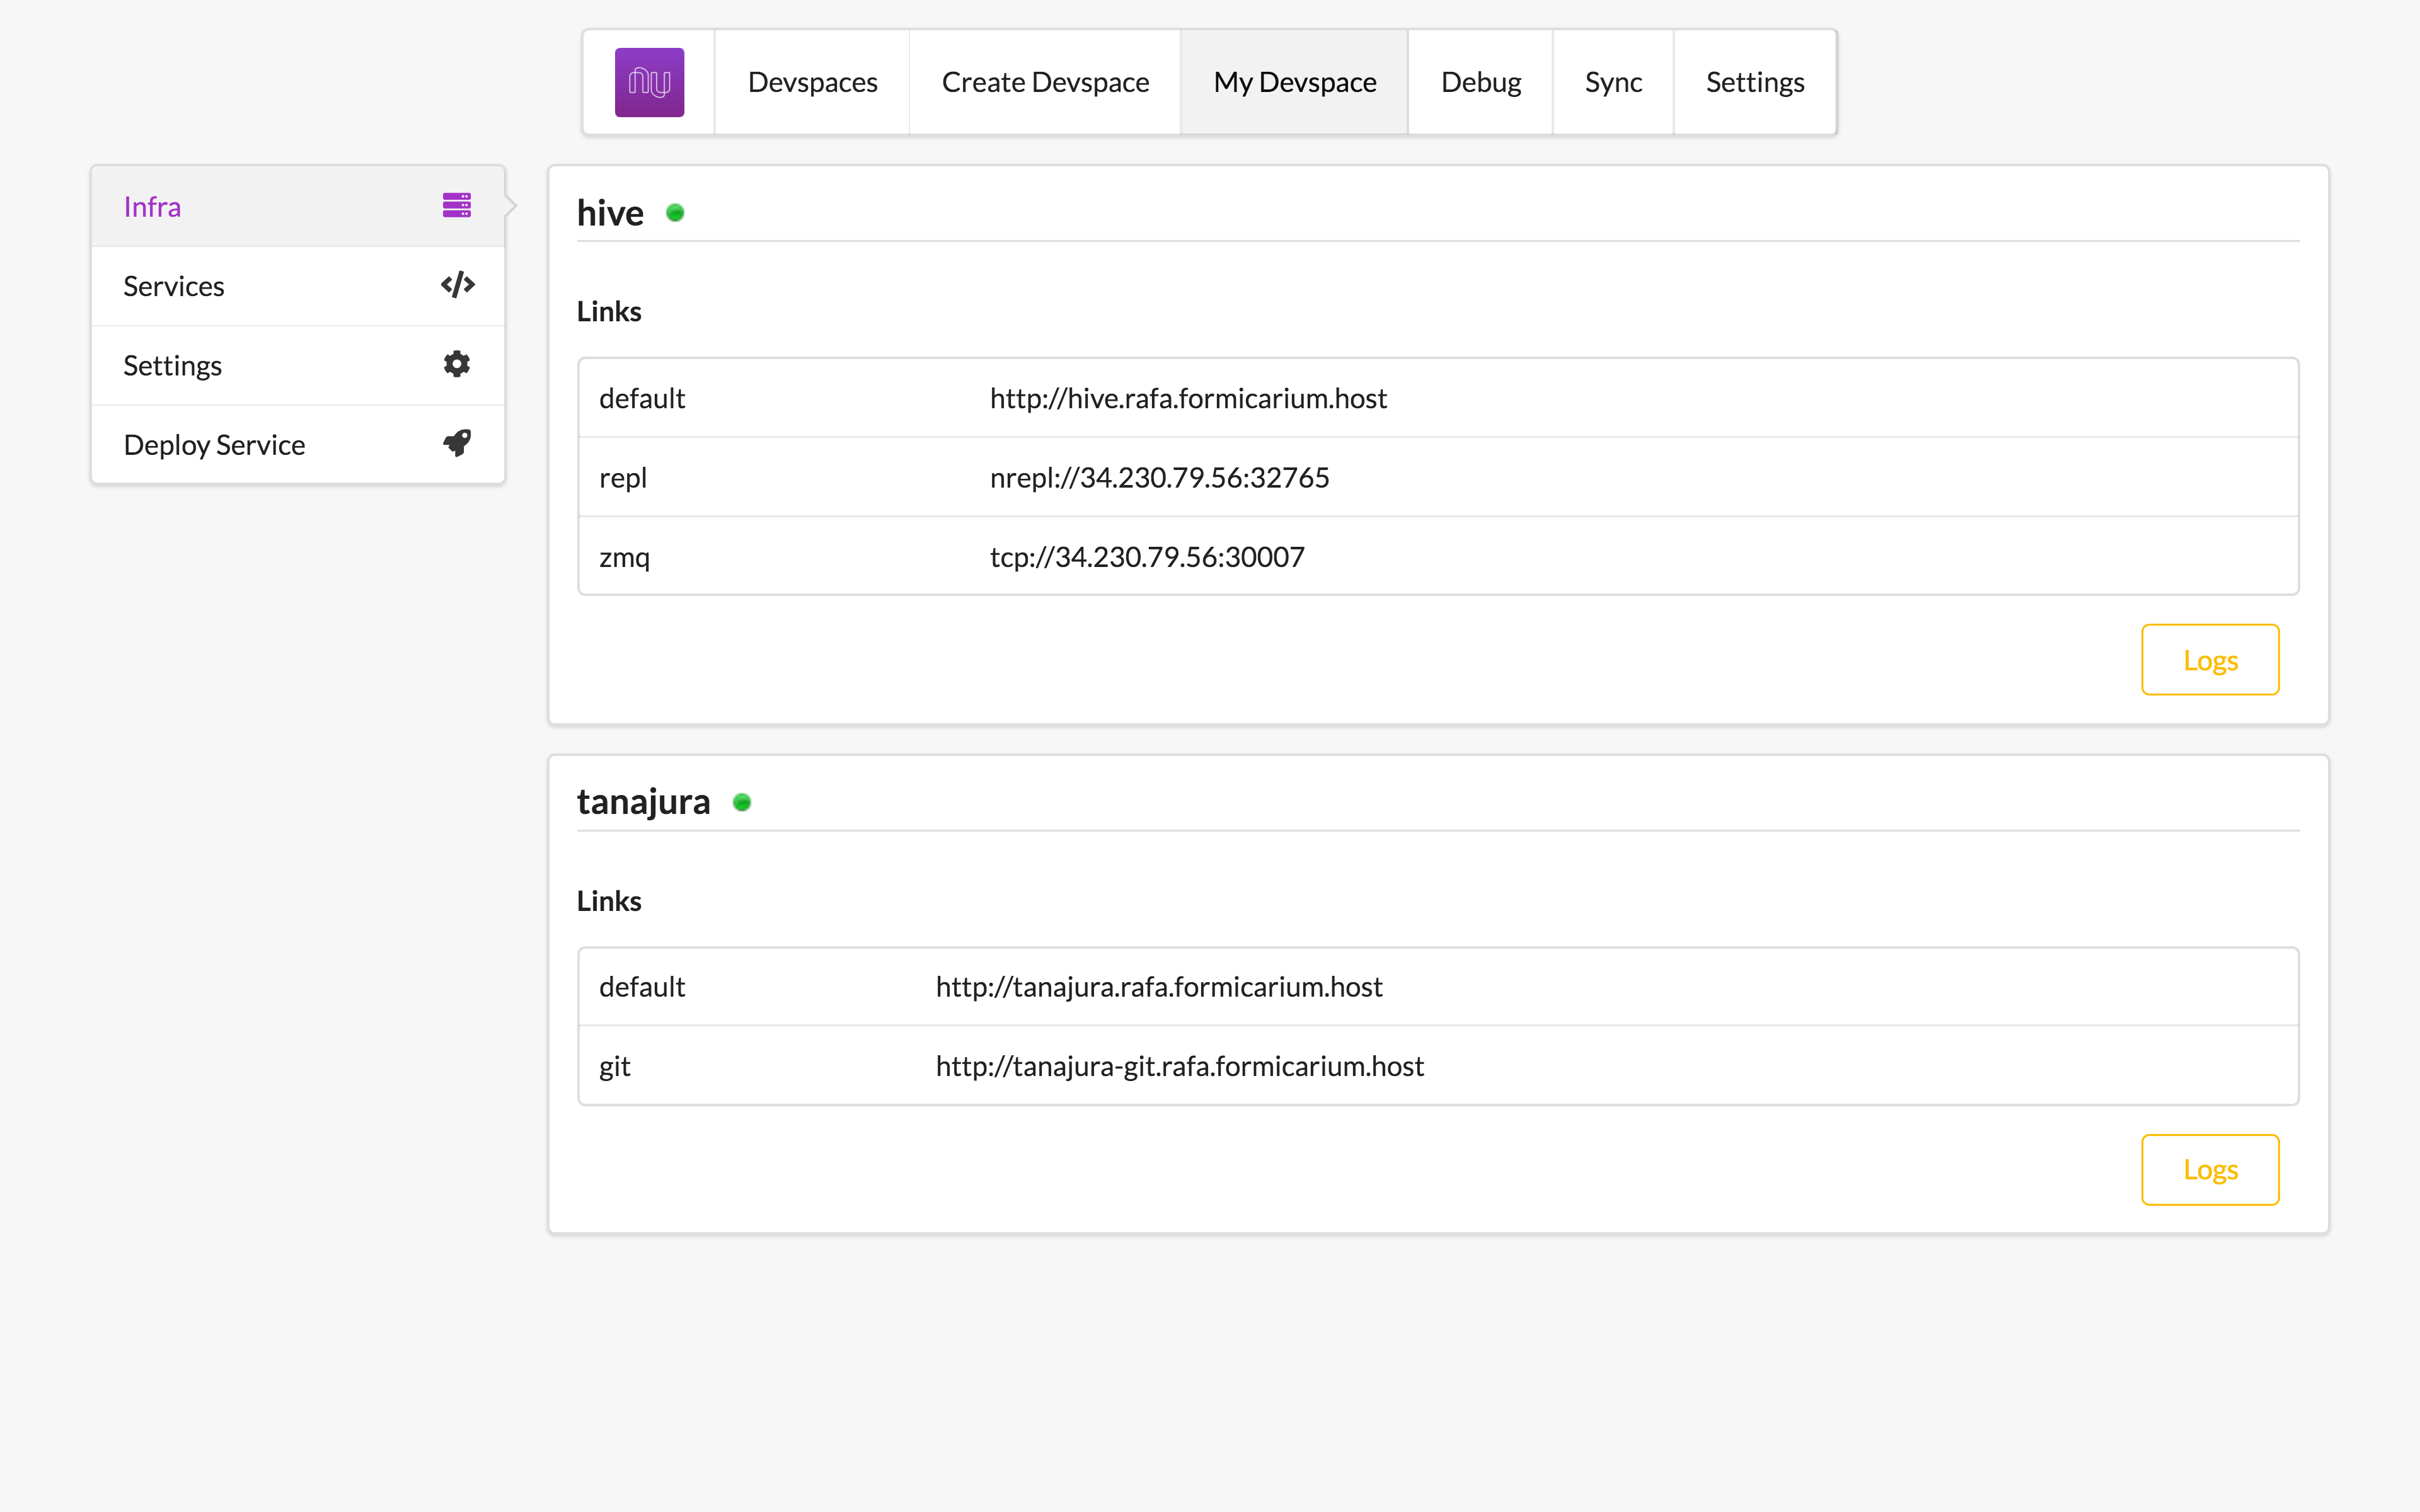
\includegraphics[width=\textwidth,keepaspectratio]{pictures/frontend/frontend-devspace-info.png}
    	\end{center}
    	\legend{Fonte: Elaborado pelos autores}
    \end{figure}
    
    \subsubsection{Serviços}
    
    Nesta área o engenheiro pode conferir o status dos serviços implantados no Devspace atual e também interagir com cada um deles de forma independente. É possível a obtenção em tempo real dos \textit{logs} (tudo que for direcionado ao \textit{stdout} e \textit{stderr} do processo), a reinicialização do processo e também a sua remoção do Devspace através de botões. A lista também apresenta as interfaces de cada processo expostas para a \textit{internet} para permitir outros tipos de interação, como por exemplo a interface de um possível servidor HTTP do serviço e a interface HTTP do Stinger, que é um gerenciador de processos oferecido pelo Formicarium e que está presente nos serviços implantados no Devspace.
    
    \begin{figure}[htb]
    	\caption{\label{fig_frontend_devspace_services}Tela Serviços do Devspace}
    	\begin{center}
    	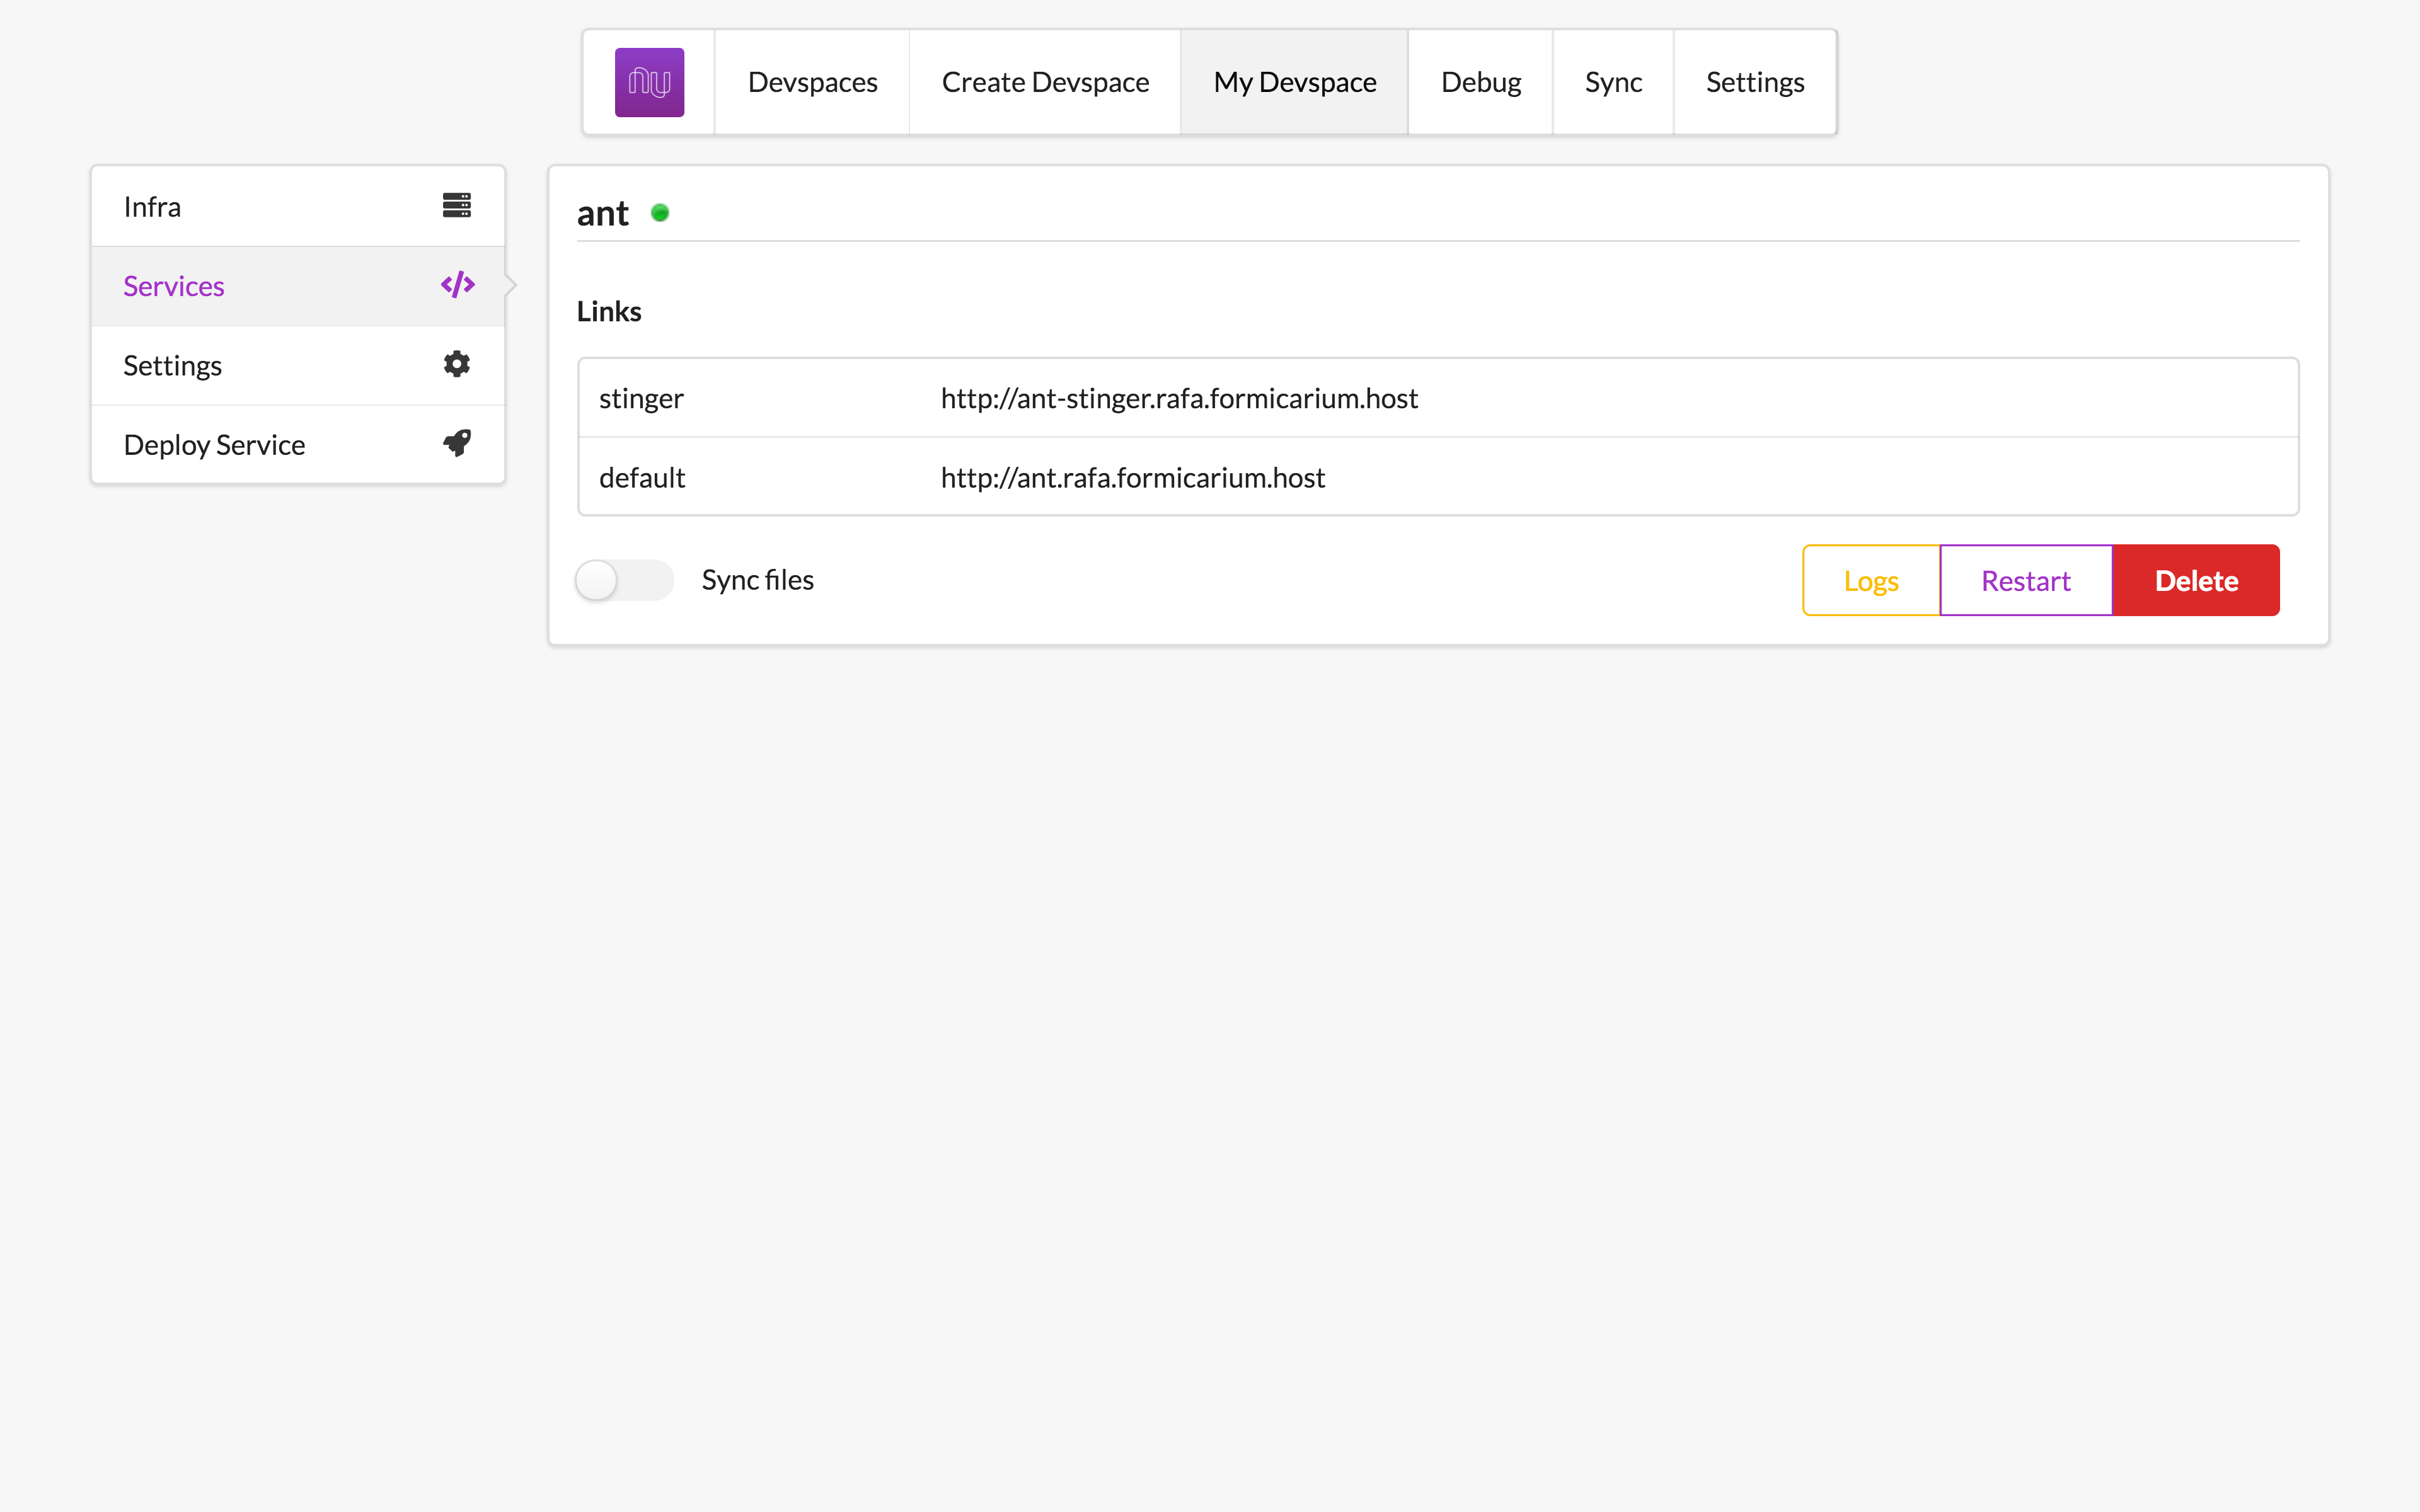
\includegraphics[width=\textwidth,keepaspectratio]{pictures/frontend/frontend-devspace-services.png}
    	\end{center}
    	\legend{Fonte: os autores - 2018-11-10}
    \end{figure}
    
    \begin{figure}[htb]
    	\caption{\label{fig_frontend_logs}Tela Logs de um serviço}
    	\begin{center}
    	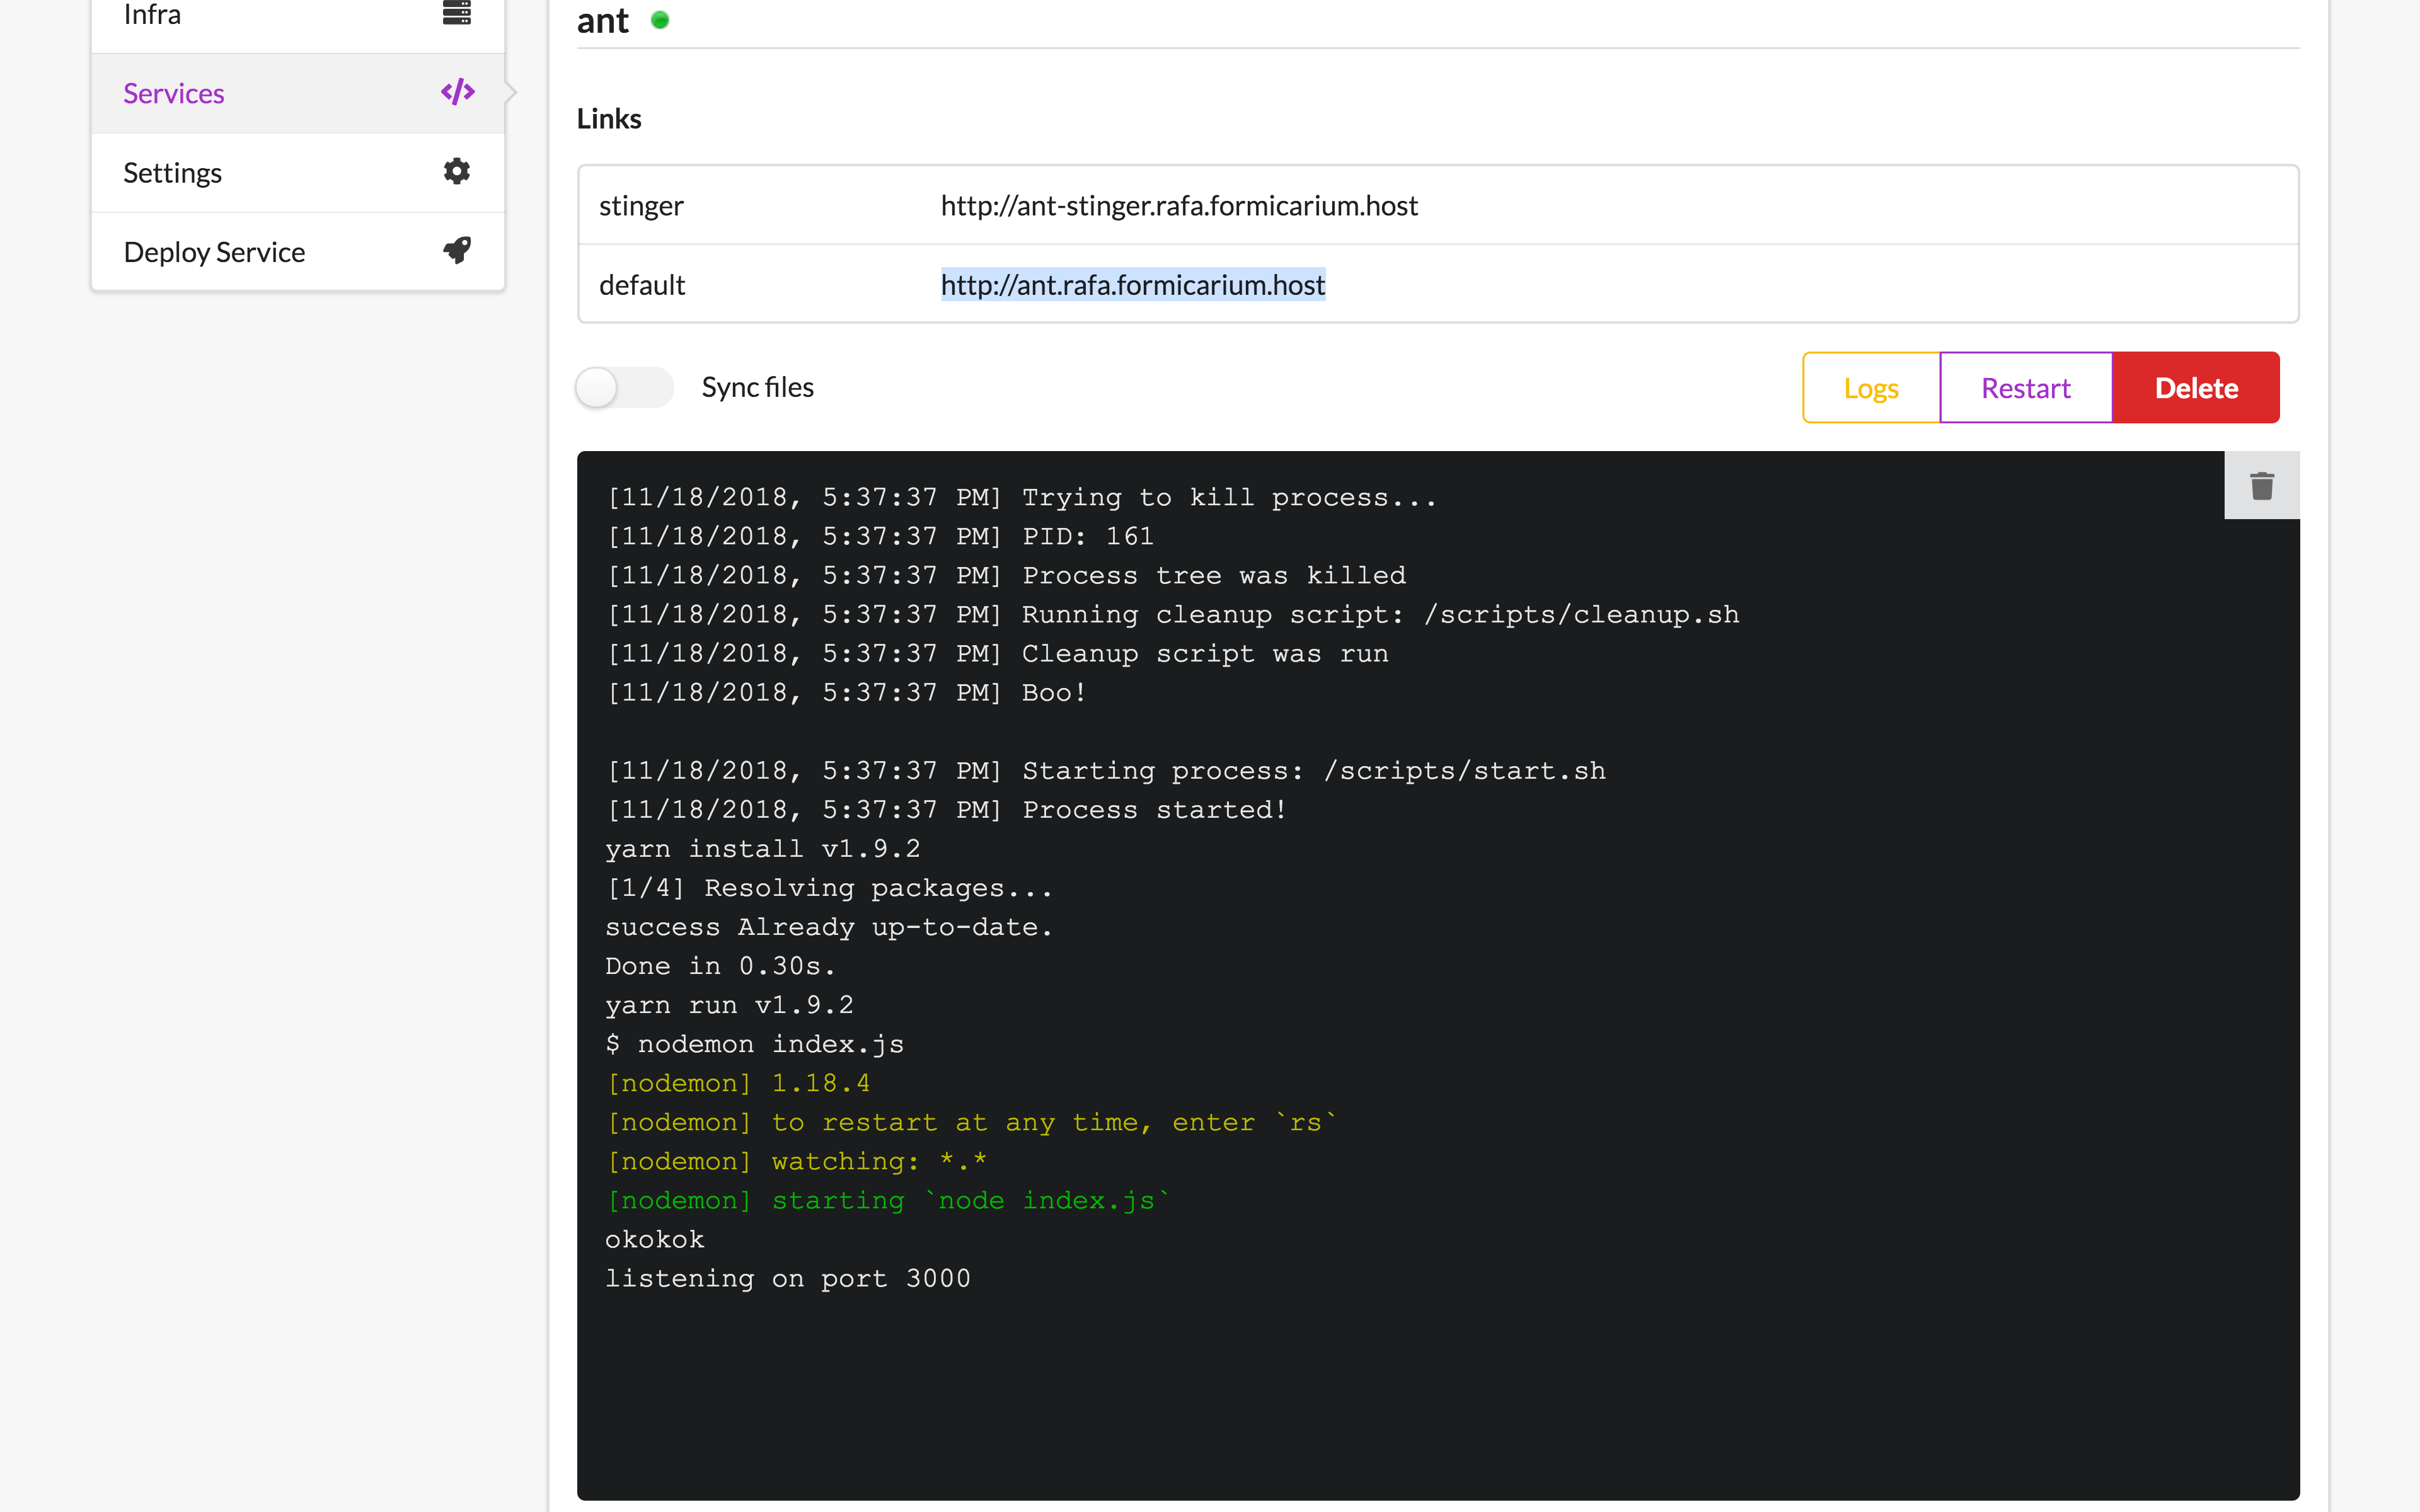
\includegraphics[width=\textwidth,keepaspectratio]{pictures/frontend/frontend-logs.png}
    	\end{center}
    	\legend{Fonte: Elaborado pelos autores}
    \end{figure}

        \subsubsection{Deploy}

            Esta área conta com um formulário para implantação de um novo serviço. É possível inserir o nome, escolher se o serviço é do tipo \textit{Syncable} (o que fará com que a imagem Docker \textit{Chamber} seja usada). Caso esta opção esteja selecionada, o engenheiro deve apontar o diretório local em que está o código fonte do serviço para que este seja enviado para o contêiner remoto e possa ser sincronizado em seguida.

% \begin{figure}[htb]
% 	\caption{\label{fig_frontnd_deploy}Tela Deploy de serviços}
% 	\begin{center}
% 	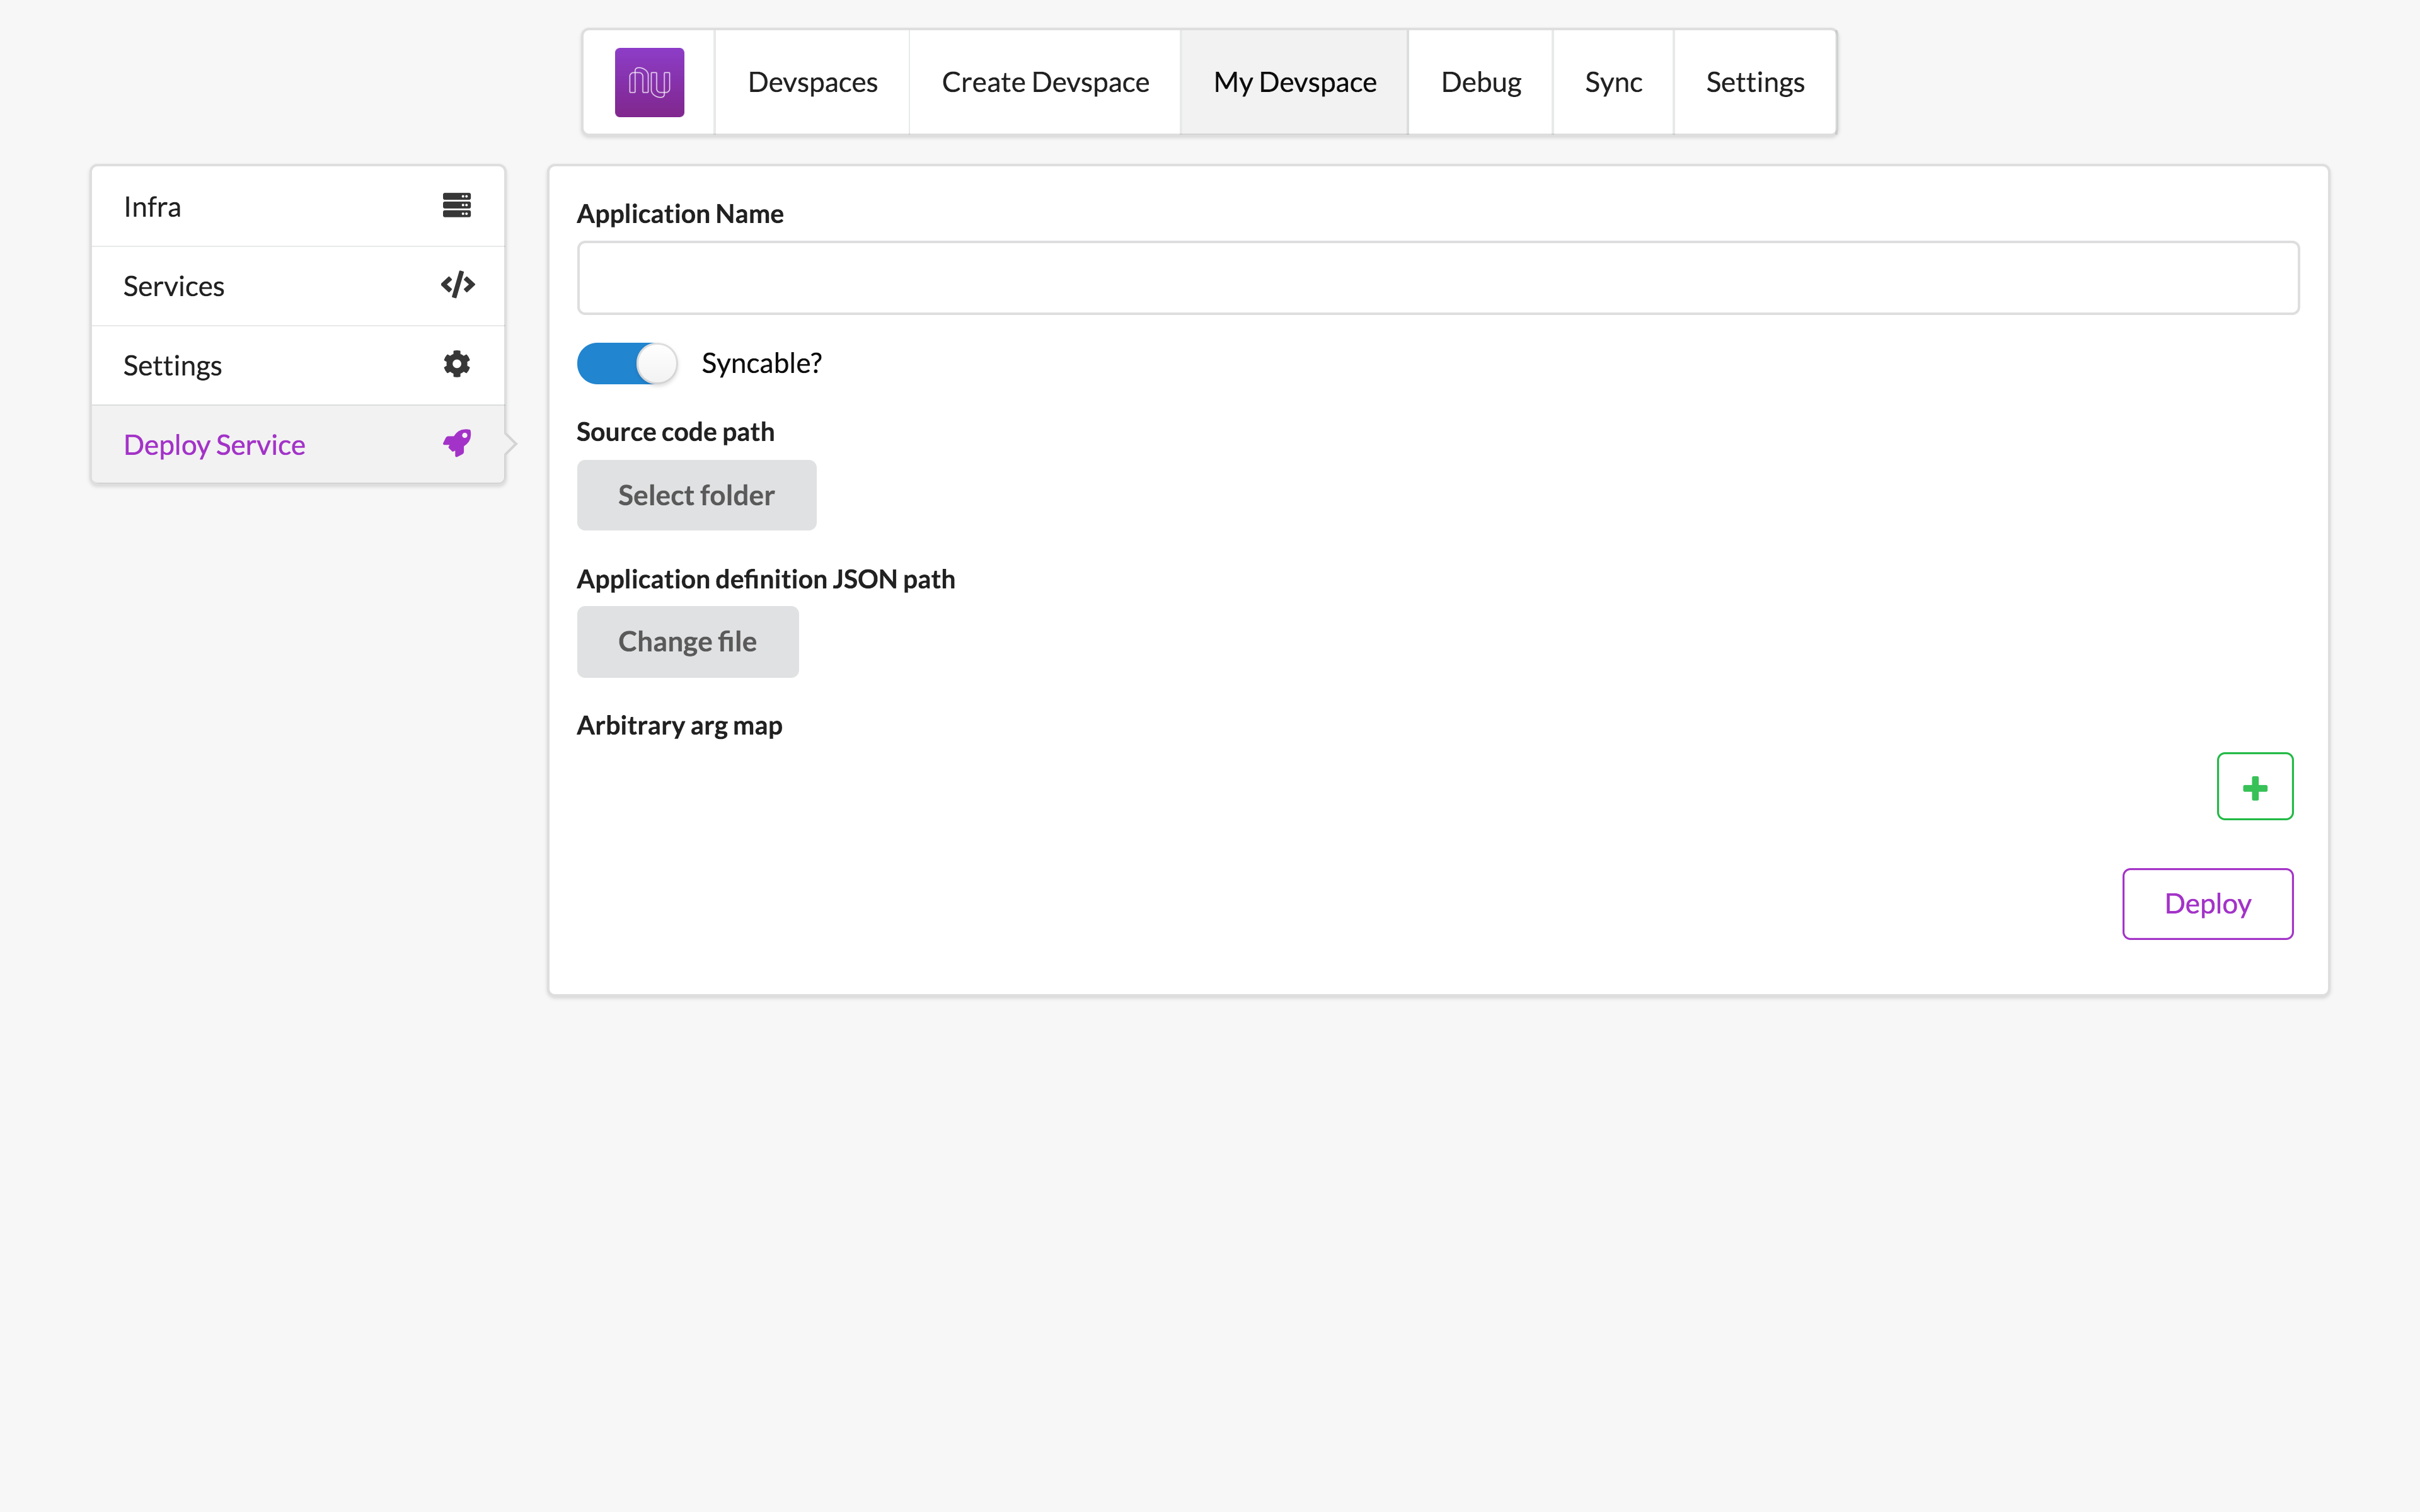
\includegraphics[width=\textwidth,keepaspectratio]{pictures/frontend/frontend-deploy.png}
% 	\end{center}
% 	\legend{Fonte: Elaborado pelos autores}
% \end{figure}

        \subsubsection{Distributed Debugger}
            Nesta interface gráfica, o engenheiro consegue visualizar as interações entre os serviços em seu devspace (ou seja, as trocas de mensagens HTTP e Kafka) através de um grafo. Este grafo é construído por um algoritmo que, através da lista de mensagens coletadas em um período pelo \textit{Hive}, determina seus nós e arestas.
            
            Os nós serão sempre os serviços envolvidos nas trocas de mensagens, enquanto que as arestas representam as interações entre estes serviços. Estas interações podem ser de diversos tipos, porém na implementação atual apenas mensagens HTTP e Kafka são corretamente interpretadas pelo sistema.
            
            Esta área conta também com uma visualização em forma de árvore, agrupando as mensagens hierarquicamente utilizando seu \textit{span id}. Este tipo de visualização ajuda a acompanhar os eventos em função de sua "profundidade". A profundidade de um evento é determinada pelo número de eventos que tiveram de ocorrer para que este fosse finalmente desencadeado.
            É possível aplicar filtros na lista de eventos para que apenas os de interesse sejam usados na geração das visualizações. Por exemplo, é possível filtrar por eventos provenientes apenas de determinados serviços ou por tipos de eventos específicos.
            
            O grafo é interativo para o usuário, ou seja, é possível movimentar com o cursor os nós e arestas para rearranjá-lo, de modo a facilitar a visualização de uma determinada região de interesse. Ao realizar um clique em uma aresta, uma nova tela com detalhes daquela interação é exibida onde o engenheiro pode obter informações completas da interação, como \textit{timestamps}, corpo e cabeçário da mensagem, remetente e destinatário, códigos de resposta, etc.

        \subsubsection{Sync}
            Nesta tela é possível visualizar os serviços que estão em modo de sincronização habilitado e acompanhar quais arquivos foram de fato sincronizados e o estado dessa operação (carregando, sucesso ou erro).



            \begin{figure}[htb]
        		\caption{\label{fig_frontend_sync}Tela Sincronização de arquivos em um serviço}
        		\begin{center}
        		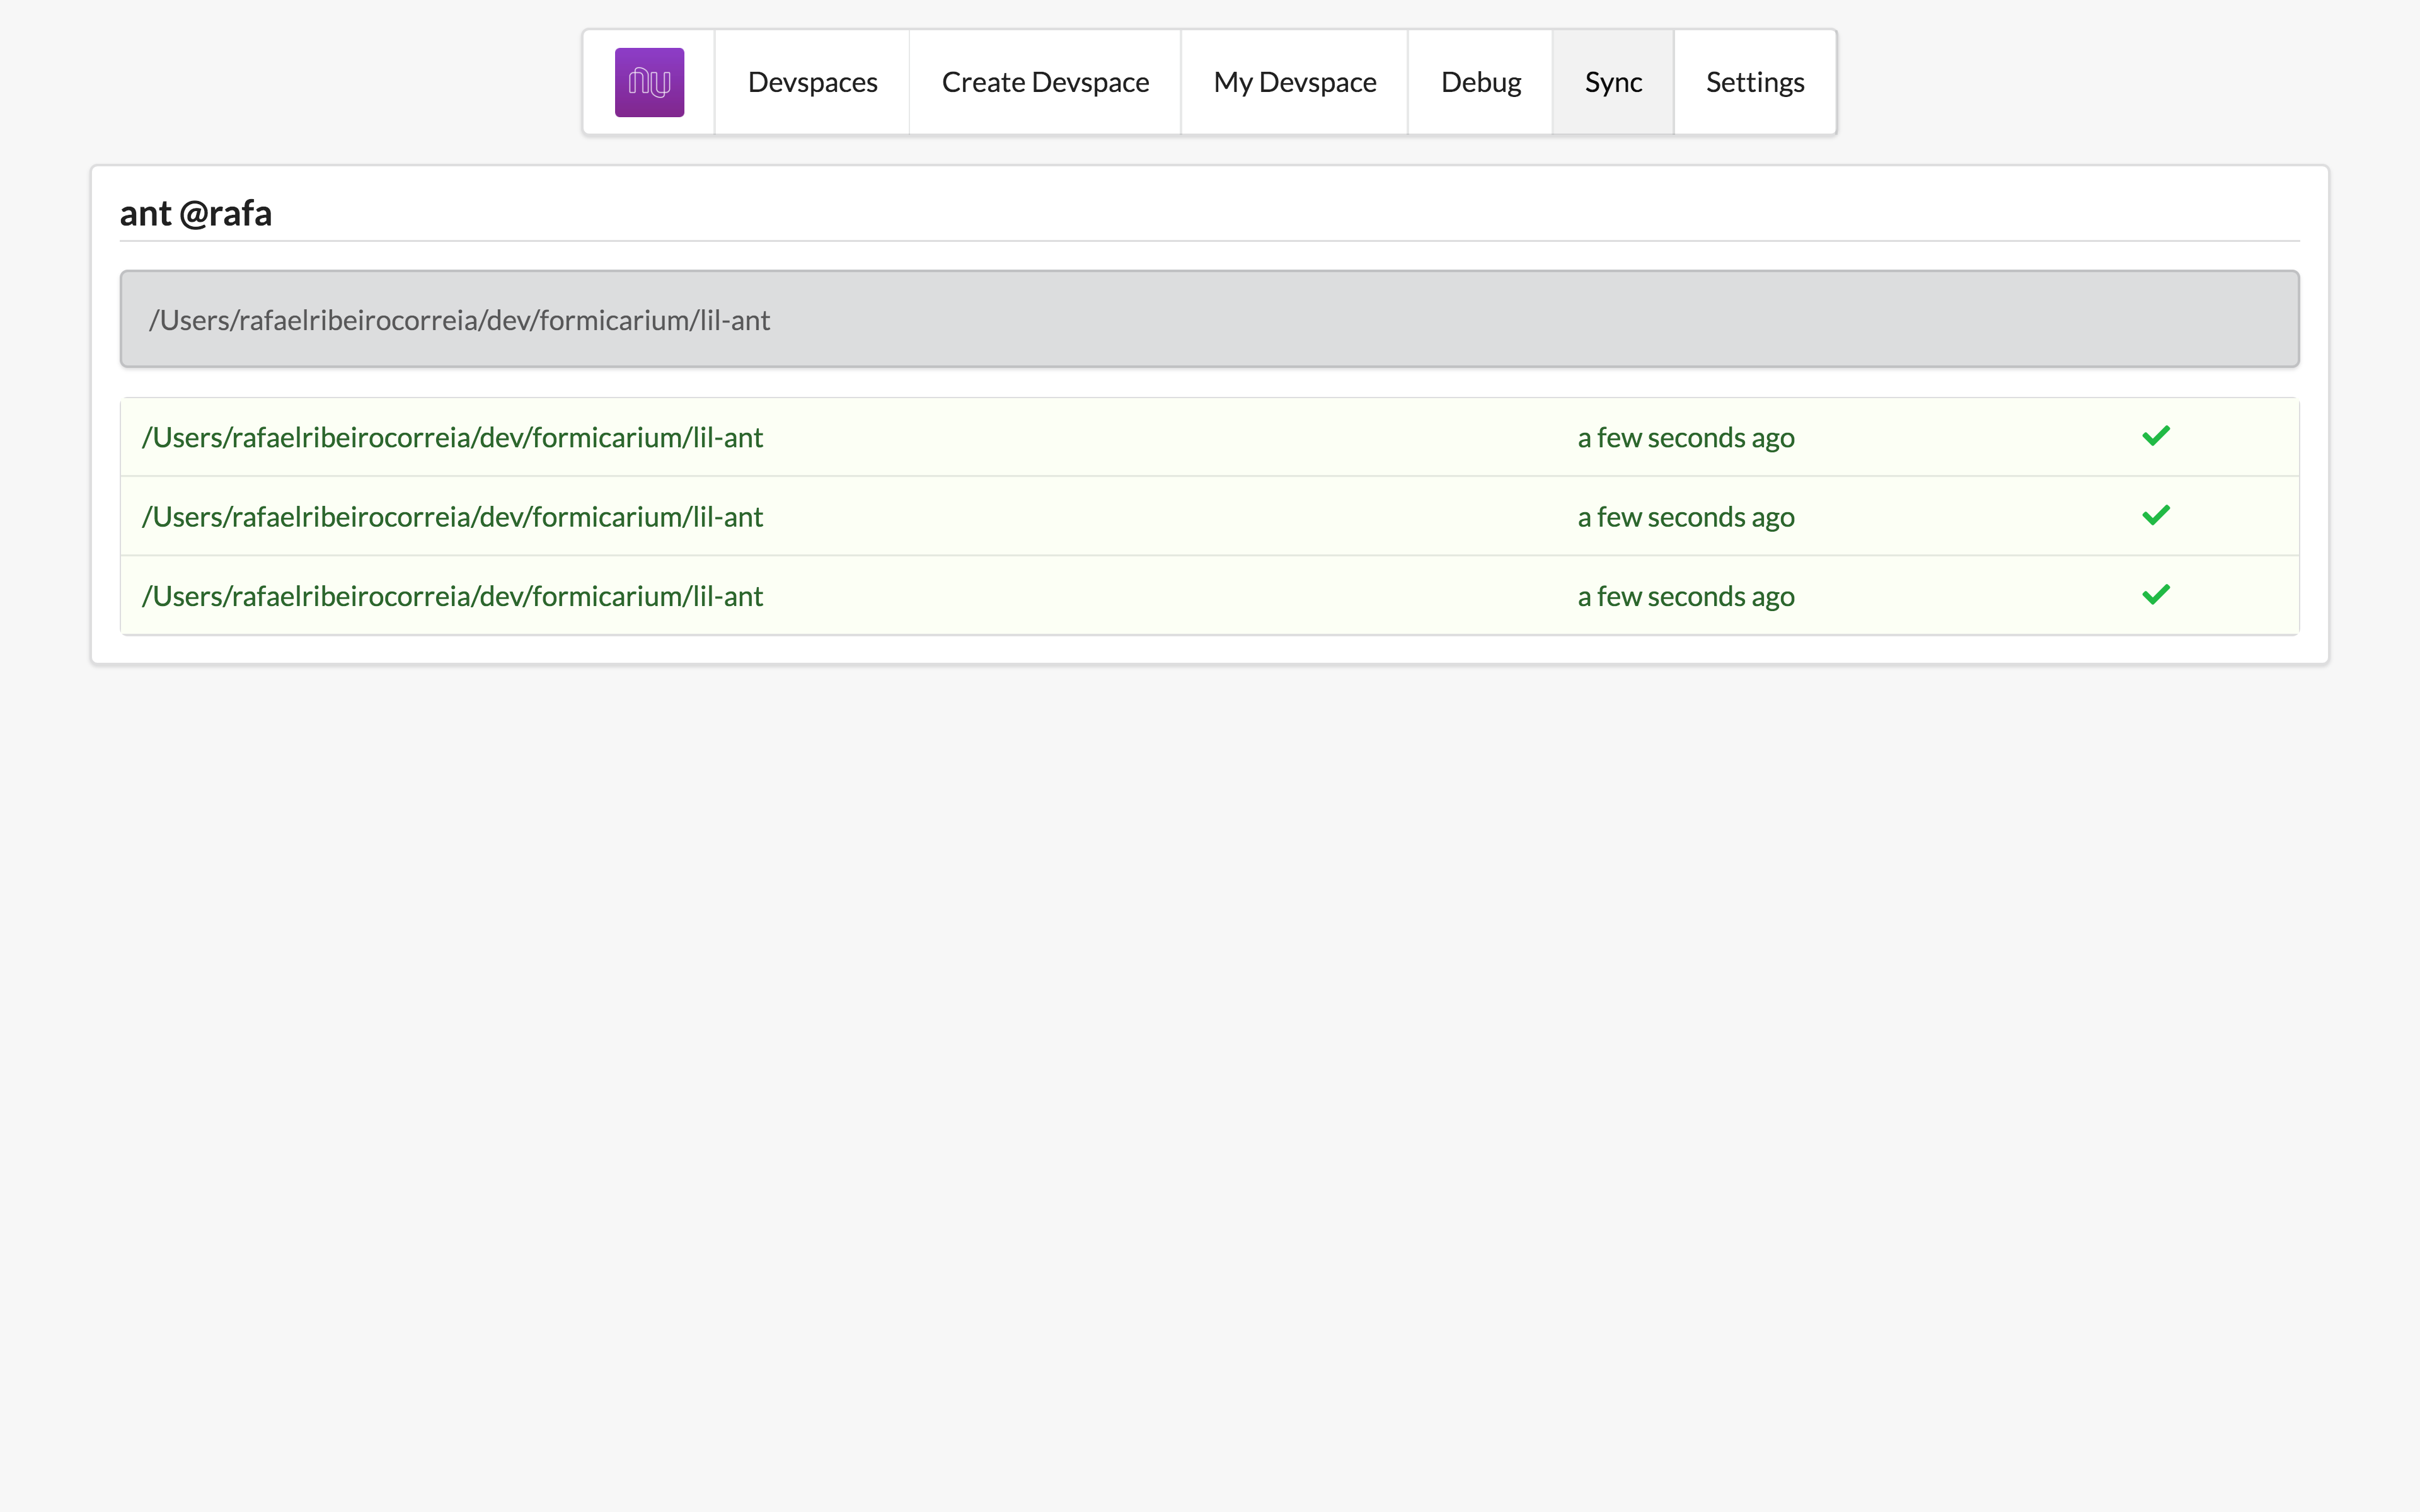
\includegraphics[width=\textwidth,keepaspectratio]{pictures/frontend/frontend-sync.png}
        		\end{center}
        		\legend{Fonte: Elaborado pelos autores}
        	\end{figure}
	
    \begin{figure}[htb]
		\caption{\label{fig_frontend_tracing_details}Tela Detalhes de uma requisição}
		\begin{center}
		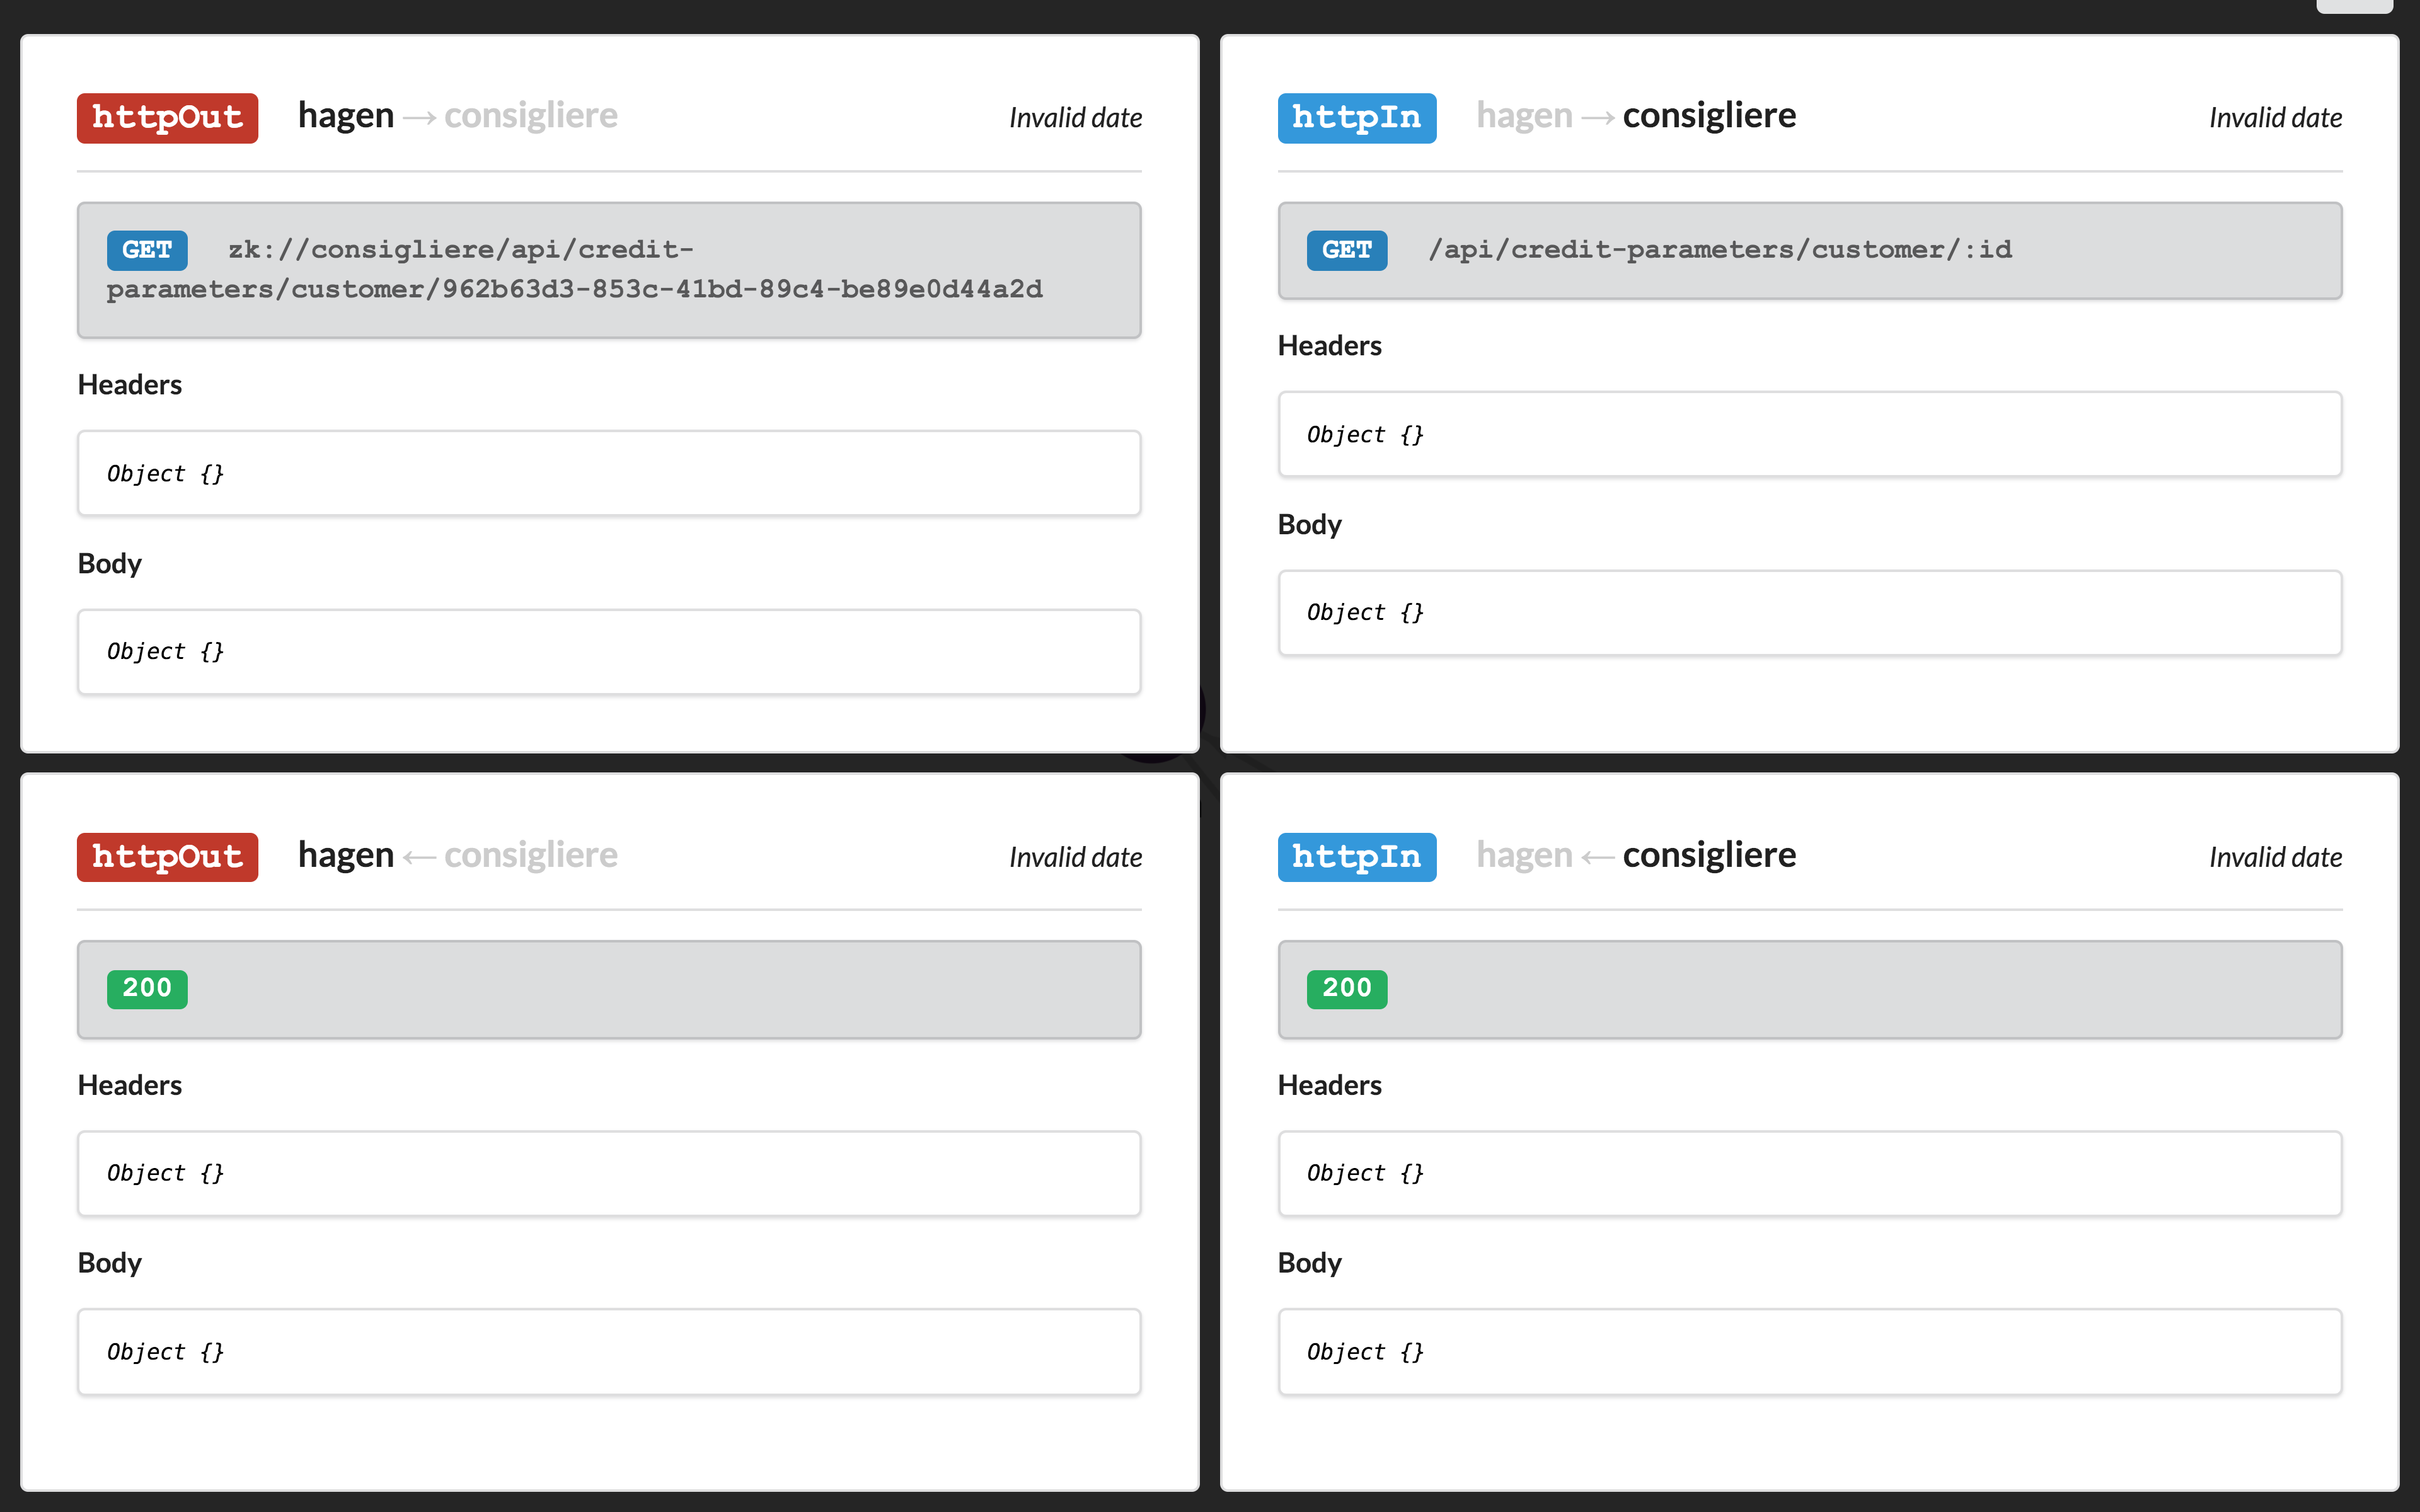
\includegraphics[width=\textwidth,keepaspectratio]{pictures/frontend/frontend-tracing-details.png}
		\end{center}
		\legend{Fonte: Elaborado pelos autores}
	\end{figure}
	
    \begin{figure}[htb]
		\caption{\label{fig_frontend_tracing}Tela Grafo de interações em Tracing}
		\begin{center}
		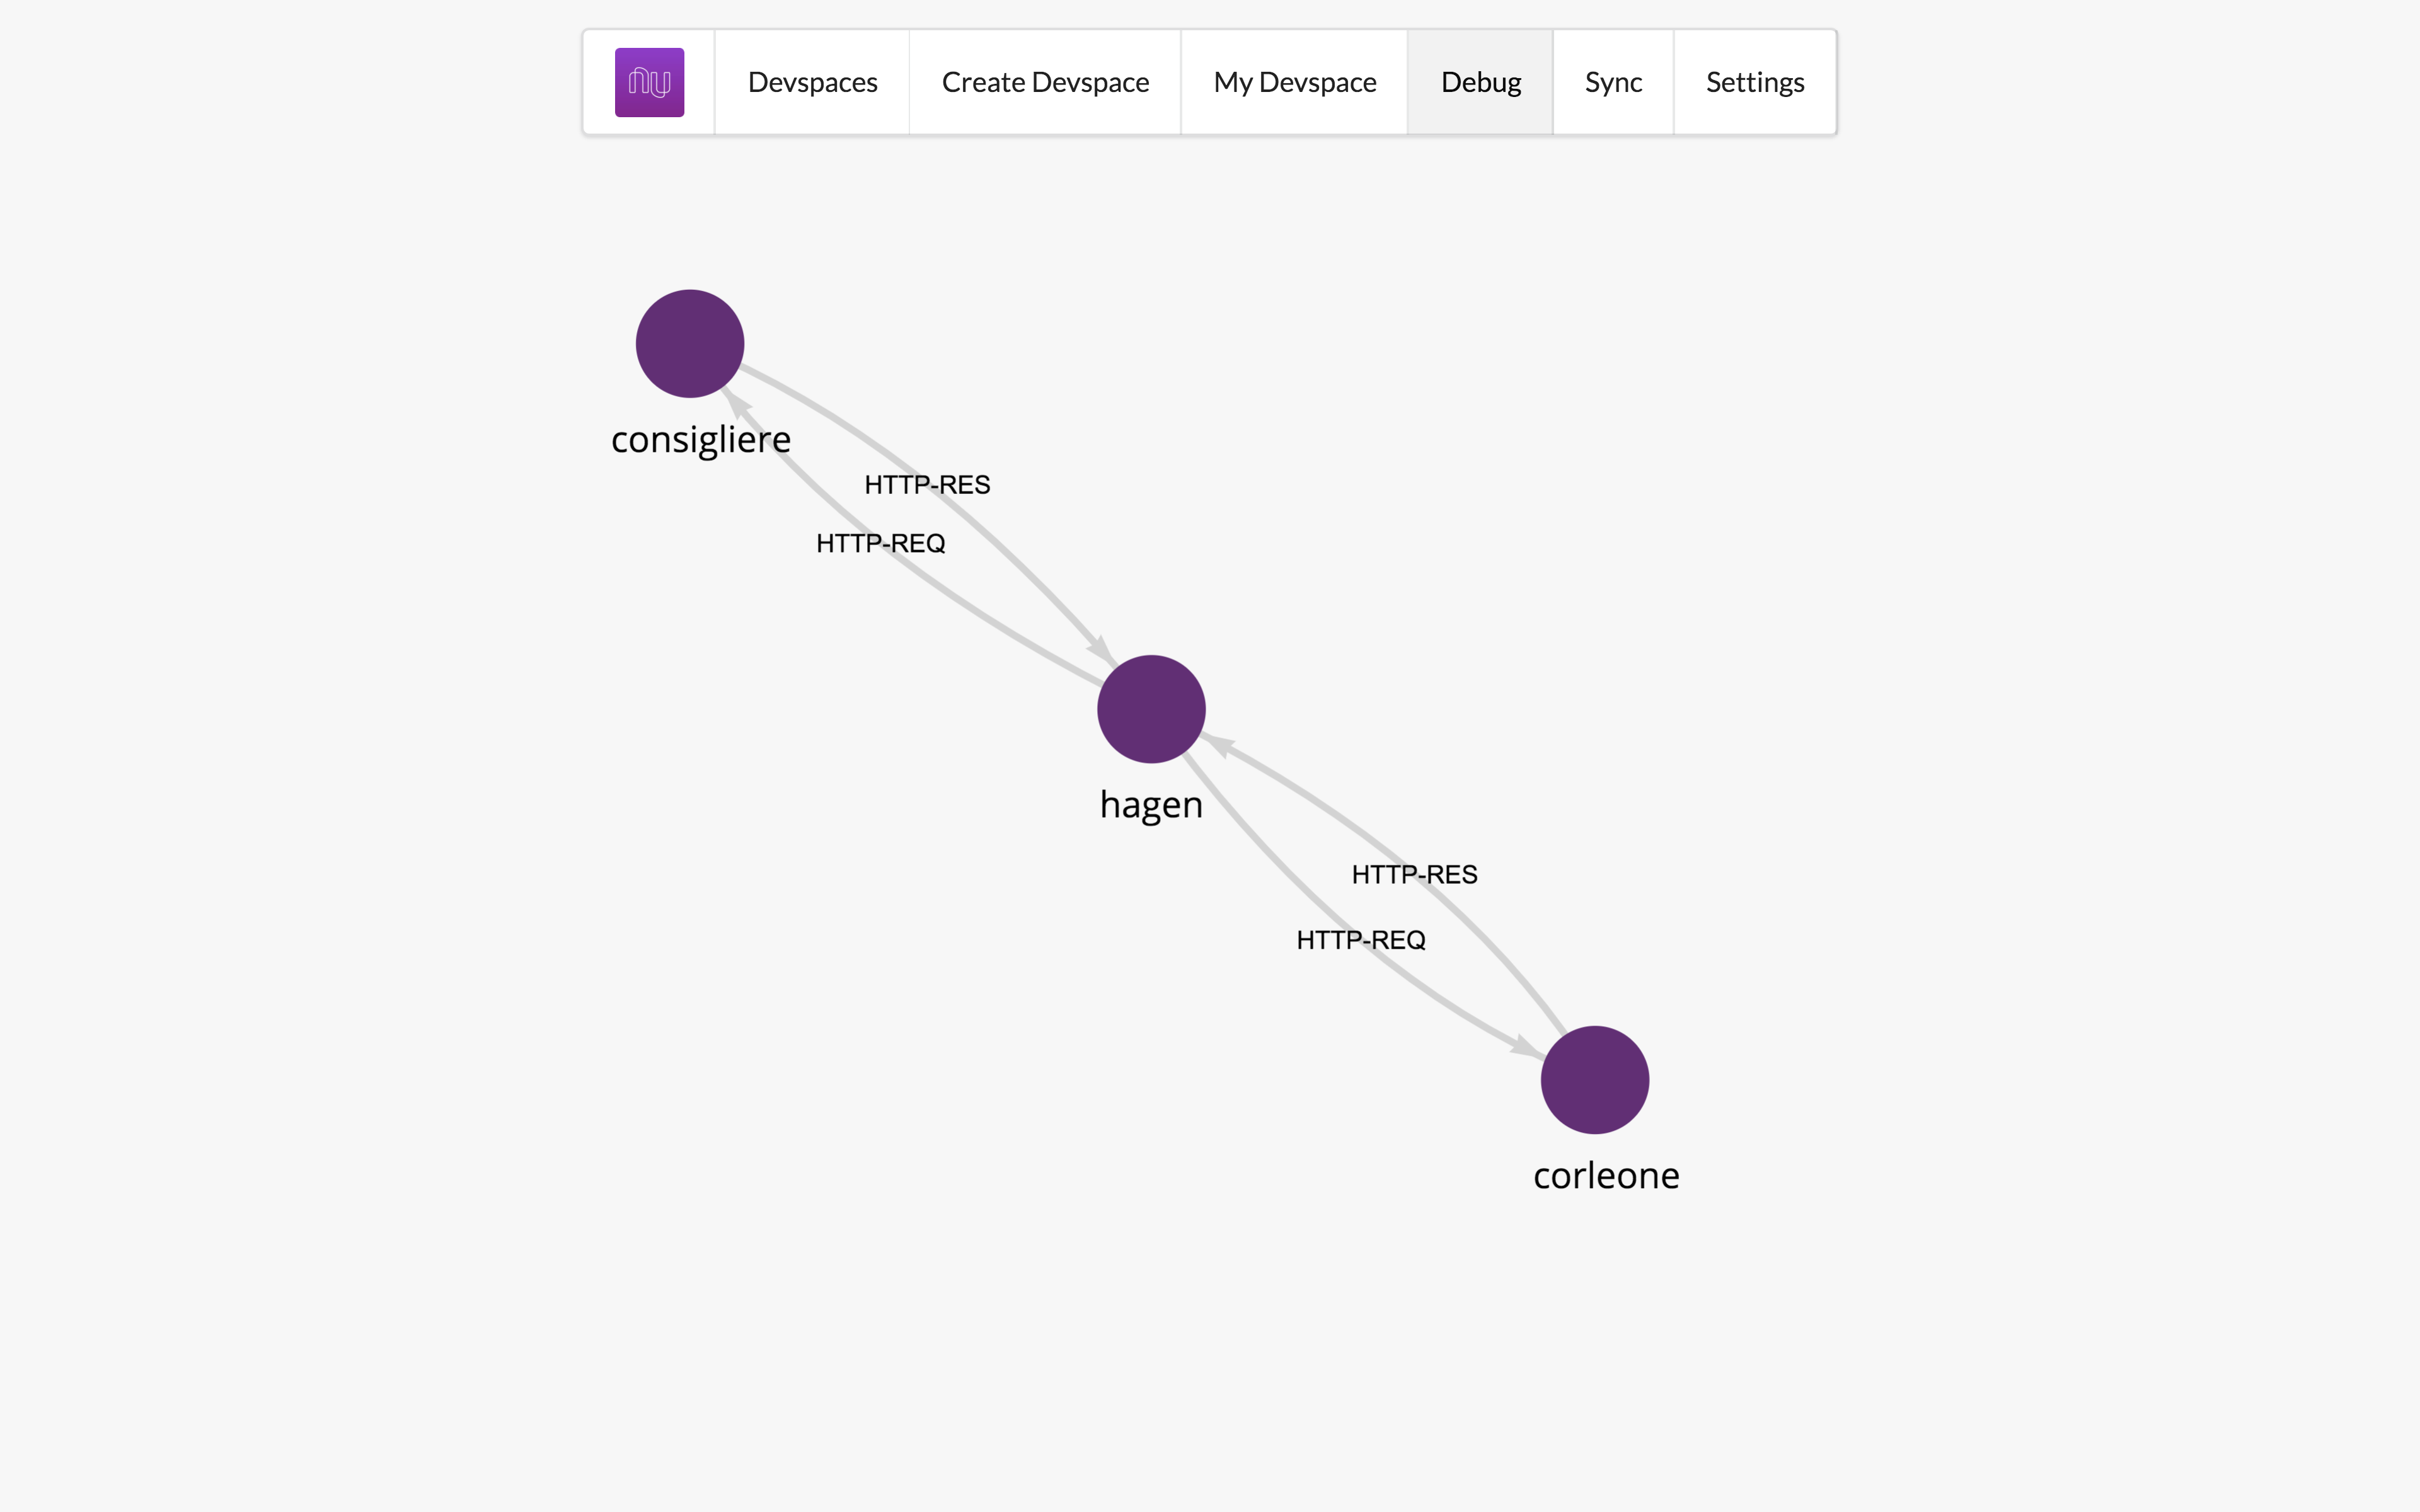
\includegraphics[width=\textwidth,keepaspectratio]{pictures/frontend/frontend-tracing.png}
		\end{center}
		\legend{Fonte: Elaborado pelos autores}
	\end{figure}

% \begin{figure}[htb]
% 		\caption{\label{fig_frontend_create_devspace}Tela Criar novo Devspace}
% 		\begin{center}
% 		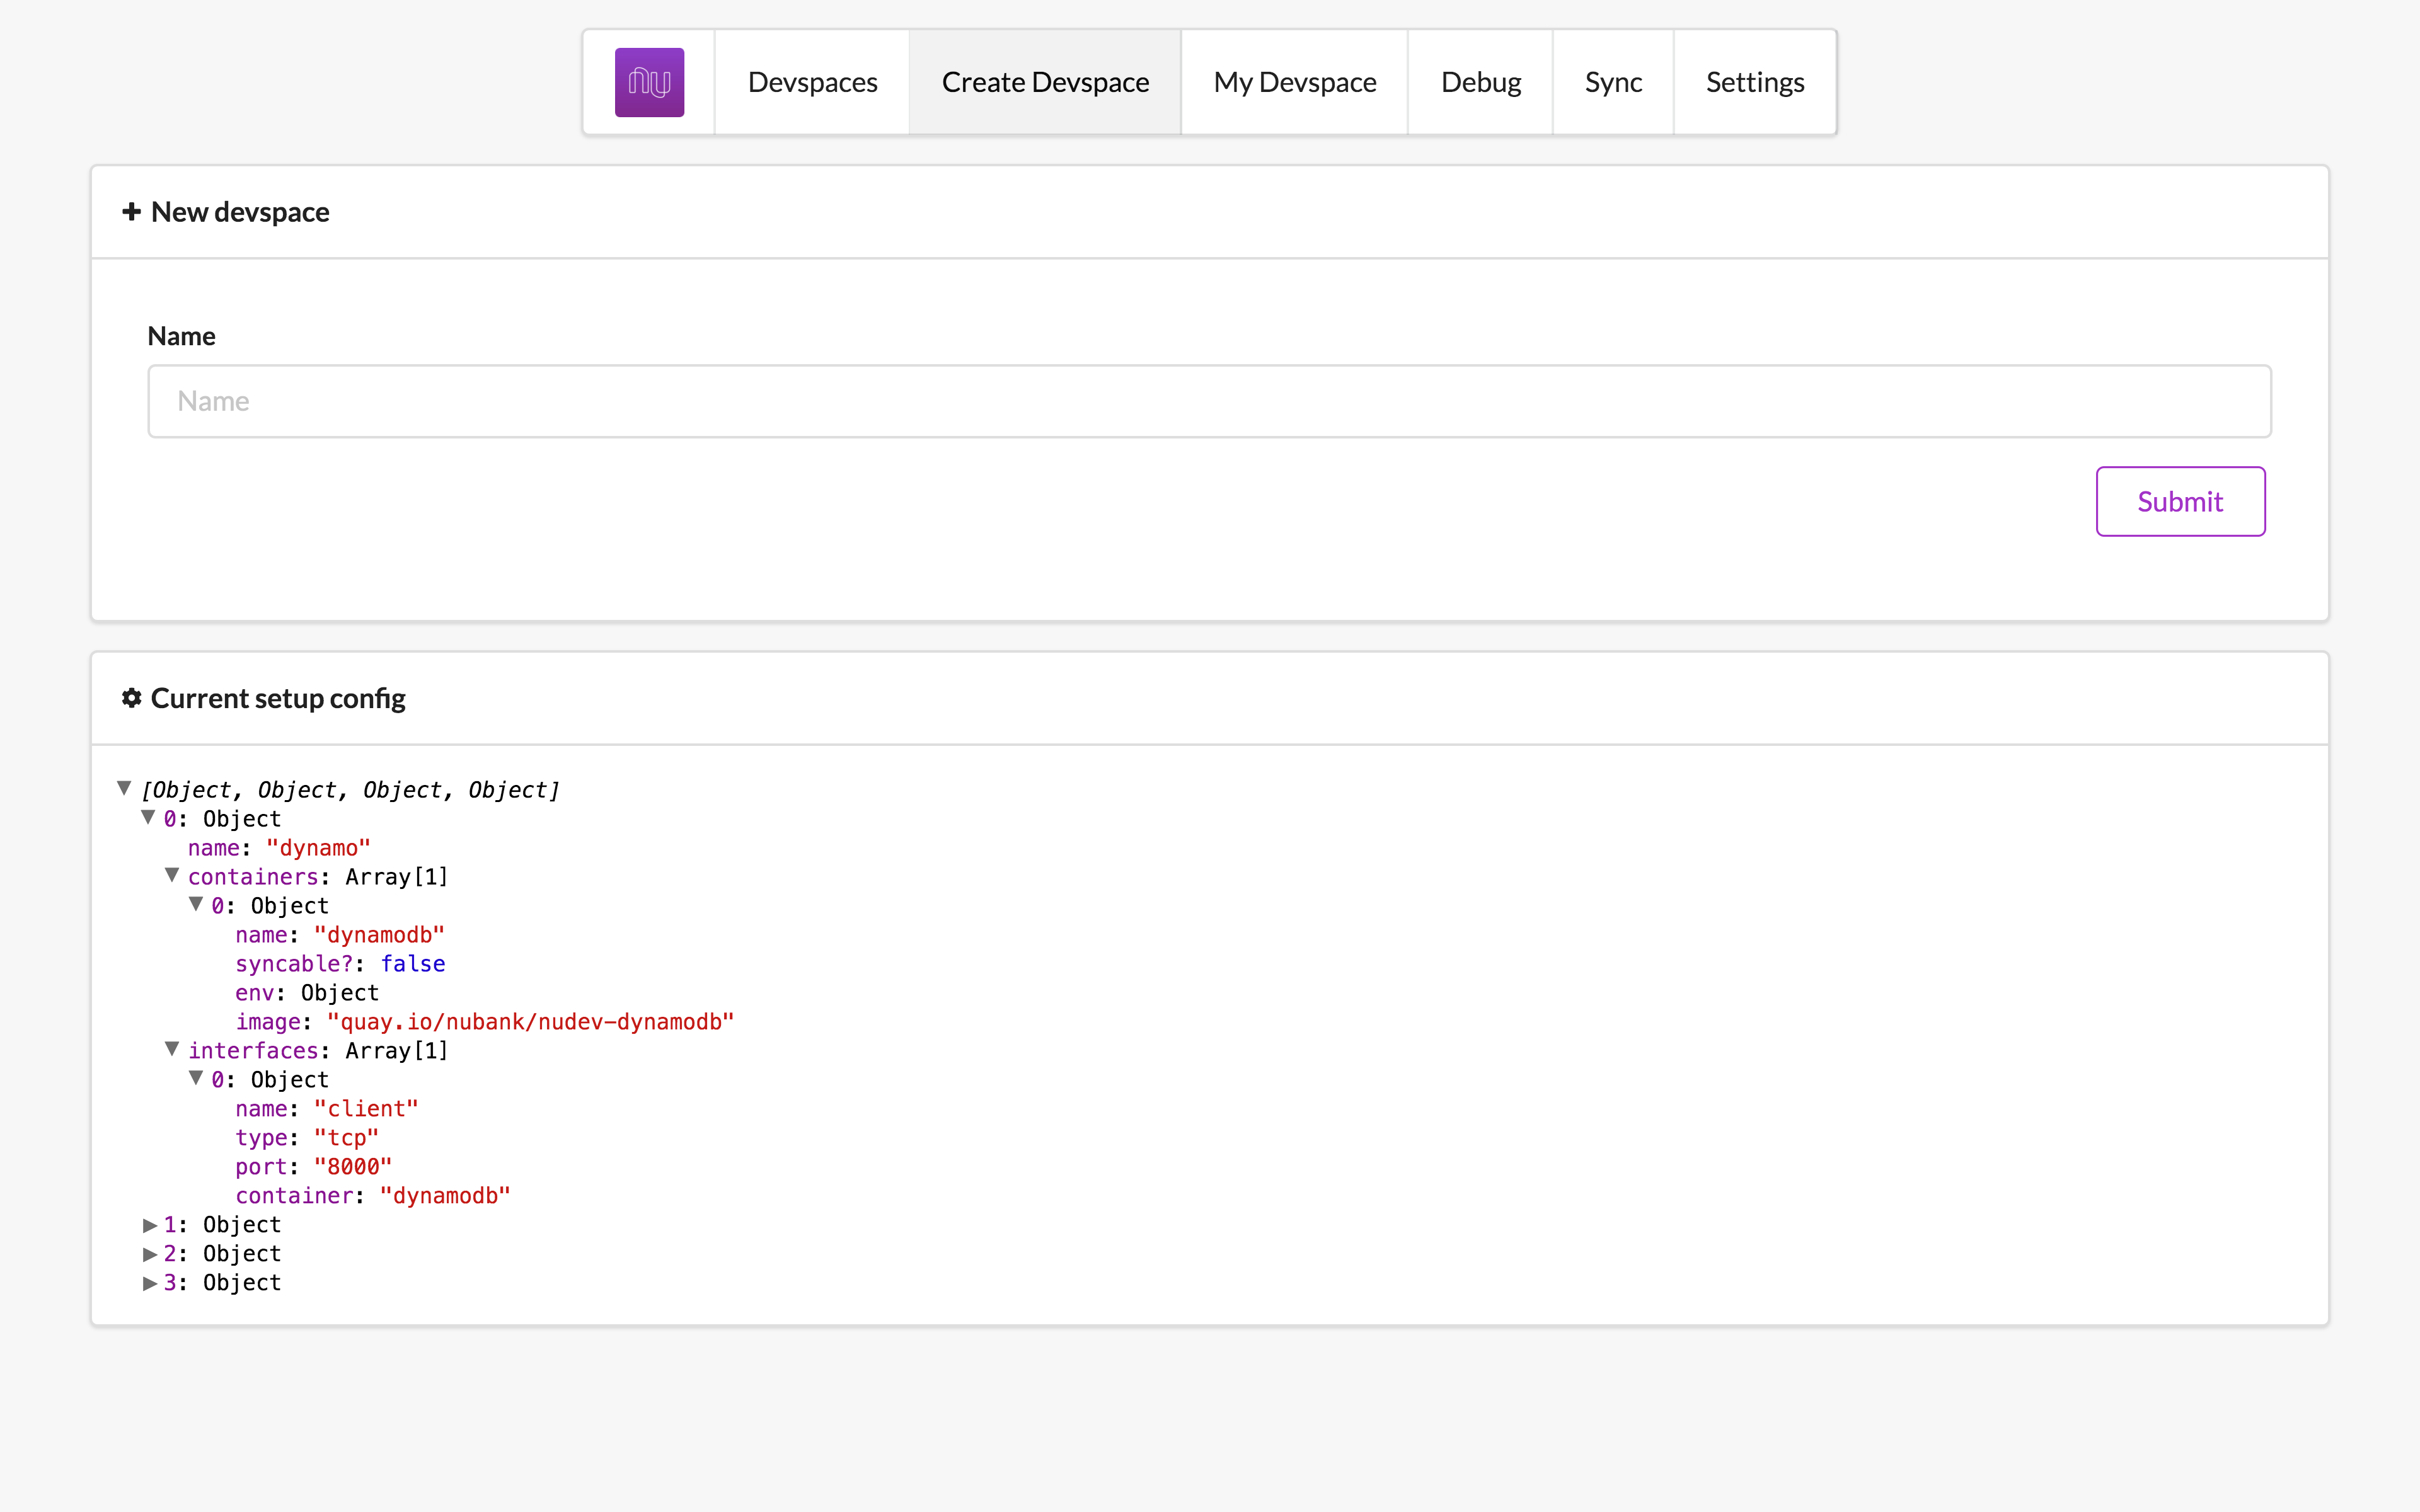
\includegraphics[width=\textwidth,keepaspectratio]{pictures/frontend/frontend-create-devspace.png}
% 		\end{center}
% 		\legend{Fonte: Elaborado pelos autores}
% 	\end{figure}


\chapter{Testes e Avaliação}\
    \section{Testes Unitários}
        Testes unitários foram feitos para por à prova pedaços específicos do código fonte de cada sistema. São muito úteis para evidenciar erros, e no caso do nosso projeto, foram feitos em escopo de função (quando a mesma apresentasse algum tipo de lógica não-trivial, como transformação de dados, criação de \textit{Devspaces}, etc). Os mesmos eram executados em tempo de desenvolvimento, e também foram feitos passos de teste no nosso ambiente de \textit{CI/CD}, permitindo que os artefatos com versões novas dos serviços e bibliotecas só pudessem ser gerados caso todos os testes unitários estivessem passando.
    
    \section{Testes Integrados}
        Testes Integrados foram feitos para por à prova um conjunto de módulos de cada \textit{microsserviço}, que no nosso caso corresponde aos módulos de banco de dados, camada \textit{web}, camada de lógica de negócio, módulo de mensageria \textit{Kafka}, dentre outras. 
        
        O teste integrado correspondeu a subir os módulos referidos, com algumas configurações simplificadas (por exemplo, banco de dados local, \textit{Kafka} \textit{mockado}, etc) e desenvolver asserções.
        
        Fizemos testes integrados no \textit{Soil} para estressar toda a manipulação de \textit{Devspaces}, simulando requisições da \textit{CLI} ou \textit{UI}, como por exemplo, um disparo no \textit{endpoint} de criar ou deletar \textit{Devspace}. 
        
        Fizemos testes integrados para o \textit{config-server} do \textit{Nubank} também, mais focados nas respostas de variáveis de ambiente e como fonte de documentação para nós mesmos adaptarmos o código do \textit{Soil} para lidar corretamente com a criação de \textit{Devspace} a partir da resposta do mesmo.
        
        No \textit{Hive}, testes de integração foram feitos para estressar todo o fluxo de eventos, desde receber um evento até servir o mesmo de resposta para a \textit{UI}.
    
    \section{Teste entre os integrantes}
        Este foi um caso simples de teste de teste de aceitação de usuário, onde os usuários eram 3 dos 4 integrantes do grupo. Foi uma experiência feita por um dos integrantes, sem avisar os outros três de que a usabilidade do \textit{Formicarium} estava sendo testada.
        
        Enquanto refatorávamos as bibliotecas de cliente usadas em um serviço do \textit{Nubank}, um dos integrantes fez uma alteração de código em um dos componentes do microsserviço, introduzindo um \textit{bug} que causava uma \textit{NullPointerException}, possível de ser evidenciada apenas em tempo de execução. Mais especificamente, o código responsável por enviar as mensagens via \textit{ZeroMQ} transforma os mapas de evento de \textit{clojure} para uma \textit{string} \textit{JSON}. A alteração foi feita para causar essa transformação falhar, e tentarmos enviar um nulo para o \textit{Hive}, causando a exceção referida. Tal cenário é impossível de ser reproduzido em testes unitários pois para os mesmos, os \textit{sockets} de \textit{ZeroMQ} são \textit{Mockados}.
        
        Com essa modificação feita, o integrante pediu ajuda do resto da equipe para resolver o problema, e a equipe foi modificando iterativamente cada parte do código para tentar encontrar o problema (a saber, colocando \textit{logs} e verificando requisições no contêiner), usando o \textit{file watch} do \textit{Formicarium}, até descobrir e resolver o problema, em cerca de 30 minutos. Ao final da experiência, o integrante responsável por introduzir o \textit{bug} comentou do experimento, e a equipe concluiu que a infraestrutura do \textit{Formicarium} facilitou o processo.
        
        Esse foi um exemplo de teste sem maiores planejamentos, porém foi uma experiência que nos permitiu por à prova se o \textit{Formicarium} de fato teria alguma utilidade prática, caso conseguisse lidar com um dos casos de erro mais comuns evidenciados no desenvolvimento de microsserviços.
    
    \section{Teste com um engenheiro do \textit{Nubank}}
        Na segunda semana de outubro, pedimos para um engenheiro do \textit{Nubank} experimentar o nosso \textit{Software}, como testador \textit{alfa}. Fizemos o \textit{setup} da máquina e nos prontificamos para lidar com quaisquer dúvidas. Ao longo de um dia de uso, o engenheiro sofreu com alguns problemas da rede local, mas conseguiu executar todas as funcionalidades do \textit{Formicarium}.
    
    \section{Implantação em um \textit{squad}}
        Em seguida, tentamos implementar o produto em uma equipe no \textit{Nubank}, onde apresentamos o produto em uma reunião e pedimos para teste dos integrantes, caso desejassem. 
        
        O produto não teve muito uso, fora os dois primeiros dias. Conversando com os integrantes para entender o motivo, identificamos que a infraestrutura e \textit{API}'s são úteis, porém fazer todo o \textit{setup} de estado inicial é muito custoso, e os engenheiros nem sempre sabem quais são os serviços envolvidos em um fluxo de negócio que desejavam aprender utilizando o \textit{Formicarium}.

\chapter{Considerações Finais}
	\section{Conclusões do Projeto de Formatura} %% TODO: Todos
	\section{Perspectivas de Continuidade}
	Mesmo com a relativa complexidade do projeto desenvolvido nessa monografia, diversos pontos se mantém abertos no \textit{backlog}, provenientes da metodologia descrita em capítulos passados desse documento. Com a completude do MVP, é esperado que esses pontos sejam atacados no ano de 2019, idealmente com os integrantes da concepção participando do desenvolvimento de forma direta ou indireta (consultiva). Quanto às perspectivas de manutenção, melhorias e desenvolvimento de novas \textit{features} do \textit{Formicarium}, alguns modos de trabalho se mostram possíveis:
	\begin{enumerate}
	    \item \textit{Squad} (com 3 a 5 engenheiros) totalmente alocados para execução destas atividades.
	    \item \textit{Pack} (2 a 5 engenheiros) dentro de um \textit{squad} horizontal (que dá suporte aos outros engenheiros, como \textit{devops}, \textit{engineering productivity}, \textit{etc.}) alocados para a execução dessas atividades.
	    \item \textit{Task Force} (pelo menos dois engenheiros), participantes de quaisquer \textit{squads}, que desenvolvem \textit{features} no tempo livre das responsabilidades e priorizações de seus \textit{squads}.
	    \item Suspensão do projeto por tempo determinado ou indeterminado.
	\end{enumerate}
	
	Supondo que a alocação de pessoas para trabalhar no projeto se mostre interessante e esteja alinhada aos interesses da empresa (o último item da lista acima não seja o escolhido), levantamos com os \textit{stakeholders} os seguintes requisitos, que agregam algum tipo de valor à experiência do usuário final (por agora não mensurados, porém com ganhos qualitativos evidentes) ou por ajudarem a manutenção e testabilidade da \textit{code base}. A descrição de alto nível dessas tarefas está a seguir:
	
	\begin{description}
  \item[Cache compartilhado de dependências]
  \hfill \\As dependência de \textit{Maven} dos microsserviços \textit{Clojure} desenvolvidos no Nubank são salvas na pasta \url{~\.m2} do contêiner alocado para execução do processo. Os testes empíricos realizados com manipulação de \textit{Devspaces} mostraram um pequeno incômodo: Quando o serviço é executado pela primeira vez no \textit{cluster}, nenhuma dependência existe no repositório mencionado. Por conta disso, toda a árvore de dependências tem que ser obtida do repositório remoto do \textit{Maven}. Este processo pode levar até 20 minutos para um serviço usual do Nubank, apesar de sincronizações futuras (utilizando o mecanismo de \textit{FileSync}) serem praticamente instantâneas.\\
  Estes 20 minutos de espera da primeira vez podem gerar frustrações, e é desejado uma experiência mais ágil de interação e desenvolvimento dos microsserviços. Para resolver este problema, uma possível solução é fazer uma espécie de \textit{cache} compartilhado dos pacotes \textit{Maven}. Como todos os \textit{Devspaces} são executados em um mesmo ambiente da empresa (a saber, \textit{stack} de teste), é possível criar um volume (utilizando o AWS \textit{Elastic Block Storage}) compartilhado por todos os \textit{Devspaces} onde a pasta \url{~\.m2} será montada. A montagem deste volume compartilhado dentro do contêiner obviamente é mais rápido do que o \textit{download} de todas as dependências através da \textit{internet}, tornando o \textit{deploy} de um serviço novo no \textit{Formicarium} muito mais rápido.
  \item[Kafka Facade Service] %% TODO: Luiz
  \hfill \\Um outro projeto de melhoria possível seria a criação de um \textit{Facade} para lidar com a \textit{API} de kafka via linha de comando ou \textit{UI}. A primeira versão do \textit{Formicarium}, descrita nessa monografia suporta apenas chamadas \textit{HTTP} como forma de iniciar um fluxo que envolve vários microsserviços. No entanto, uma coisa muito corrente que se deseja avaliar enquanto se lida com microsserviços é a maneira como o mesmo "altera o mundo" (eg, mudanças de estado, chamadas de API, mensagens enviadas, \textit{logs} reportados, etc) a partir do consumo de uma mensagem \textit{Kafka}. O \textit{Formicarium} provê facilmente para o desenvolvedor apenas a interação via \textit{HTTP}. Engenheiros mais versados em infraestrutura de \textit{Kafka} poderão lidar com o consumo de mensagens para iniciar um fluxo no \textit{Devspace} usando a \textit{API} nativa do \textit{Kafka}, mas este é um processo cansativo e propenso a erros.\\
  Para lidar com isso, pensamos na criação de um serviço para servir como \textit{Facade} para a \textit{API} nativa do \textit{Kafka}, expondo via \textit{HTTP} uma simplificação/agregação das funcionalidades expostas nos binários de implementação de \textit{Kafka}. Com o suporte nativo dado pelo \textit{Formicarium} para \textit{HTTP} ficaria simples de portar essas chamadas ao \textit{Facade} na \textit{UI} e na \textit{CLI}. Vale apontar que esse \textit{Facade} tem valor de negócio para a empresa independentemente do \textit{Formicarium}, pois facilita a interação direta dos desenvolvedores para uma das entradas de dados de seus microsserviços.
  \item[Arquivo de descrição de fluxo de negócio]
  \hfill \\Na implementação corrente o \textit{Formicarium} não provê uma maneira de fazer \textit{deploy} simultâneo de diversos serviços "de uma vez". Isso quer dizer que, para testar a interação de diversos microsserviços, hoje o usuário do \textit{Formicarium} terá que saber a priori, todos os serviços envolvidos no fluxo e subir todos, um a um. Um projeto possível de extensão do \textit{Formicarium} com bastante valor seria criar uma funcionalidade que permitisse a descrição de \textbf{Fluxos de Negócio} (conjunção de vários serviços), descritos num arquivo com formatação específica (podendo ser \textit{yaml}, \textit{xml}, \textit{json}, etc).
  \\Só isso já economizaria bastante tempo do desenvolvedor, que daria um único comando para fazer \textit{deploy} de diversos serviços e não precisaria conhecer todos, a priori.
  \\Com isso funcionando, uma \textit{feature} de exportagem e compartilhamento de fluxos, compostos por um conjunto de serviços e versões específicas dos mesmos seria possível, dando ainda maior poder e autonomia para os engenheiros pensarem em modificações e impactos das mesmas na lógica de negócio que envolve mais de um serviço. 
  \item[Flamegraph] %% TODO: Luiz
  \hfill \\Flamegraph é um tipo de gráfico bastante interessante para representação temporal de um fluxo de eventos (opcionalmente independentes entre si). Ele demonstra o tempo gasto processando cada evento, exatamente na ordem em que os eventos foram processados. A figura \ref{fig:flamegraph-example} mostra um exemplo de \textit{flamegraph}.\\
	Hoje o \textit{Formicarium} provê apenas uma visualização de grafo de acontecimento dos eventos, que é muito bom para ver a estrutura de chamadas e os serviços envolvidos, mas deixa um pouco a desejar quando o usuário quer ter um detalhamento mais granular nos tempos de processamento envolvidos. Nesse contexto, implementar uma visualização de \textit{Flamegraph} para os eventos se mostraria vantajoso pois estenderia as possibilidades de \textit{debugging} de um conjunto de eventos providas pelo \textit{Formicarium}.
	\begin{figure}[htb]
		\caption{\label{fig:flamegraph-example}Exemplo de flamegraph}
		\begin{center}
		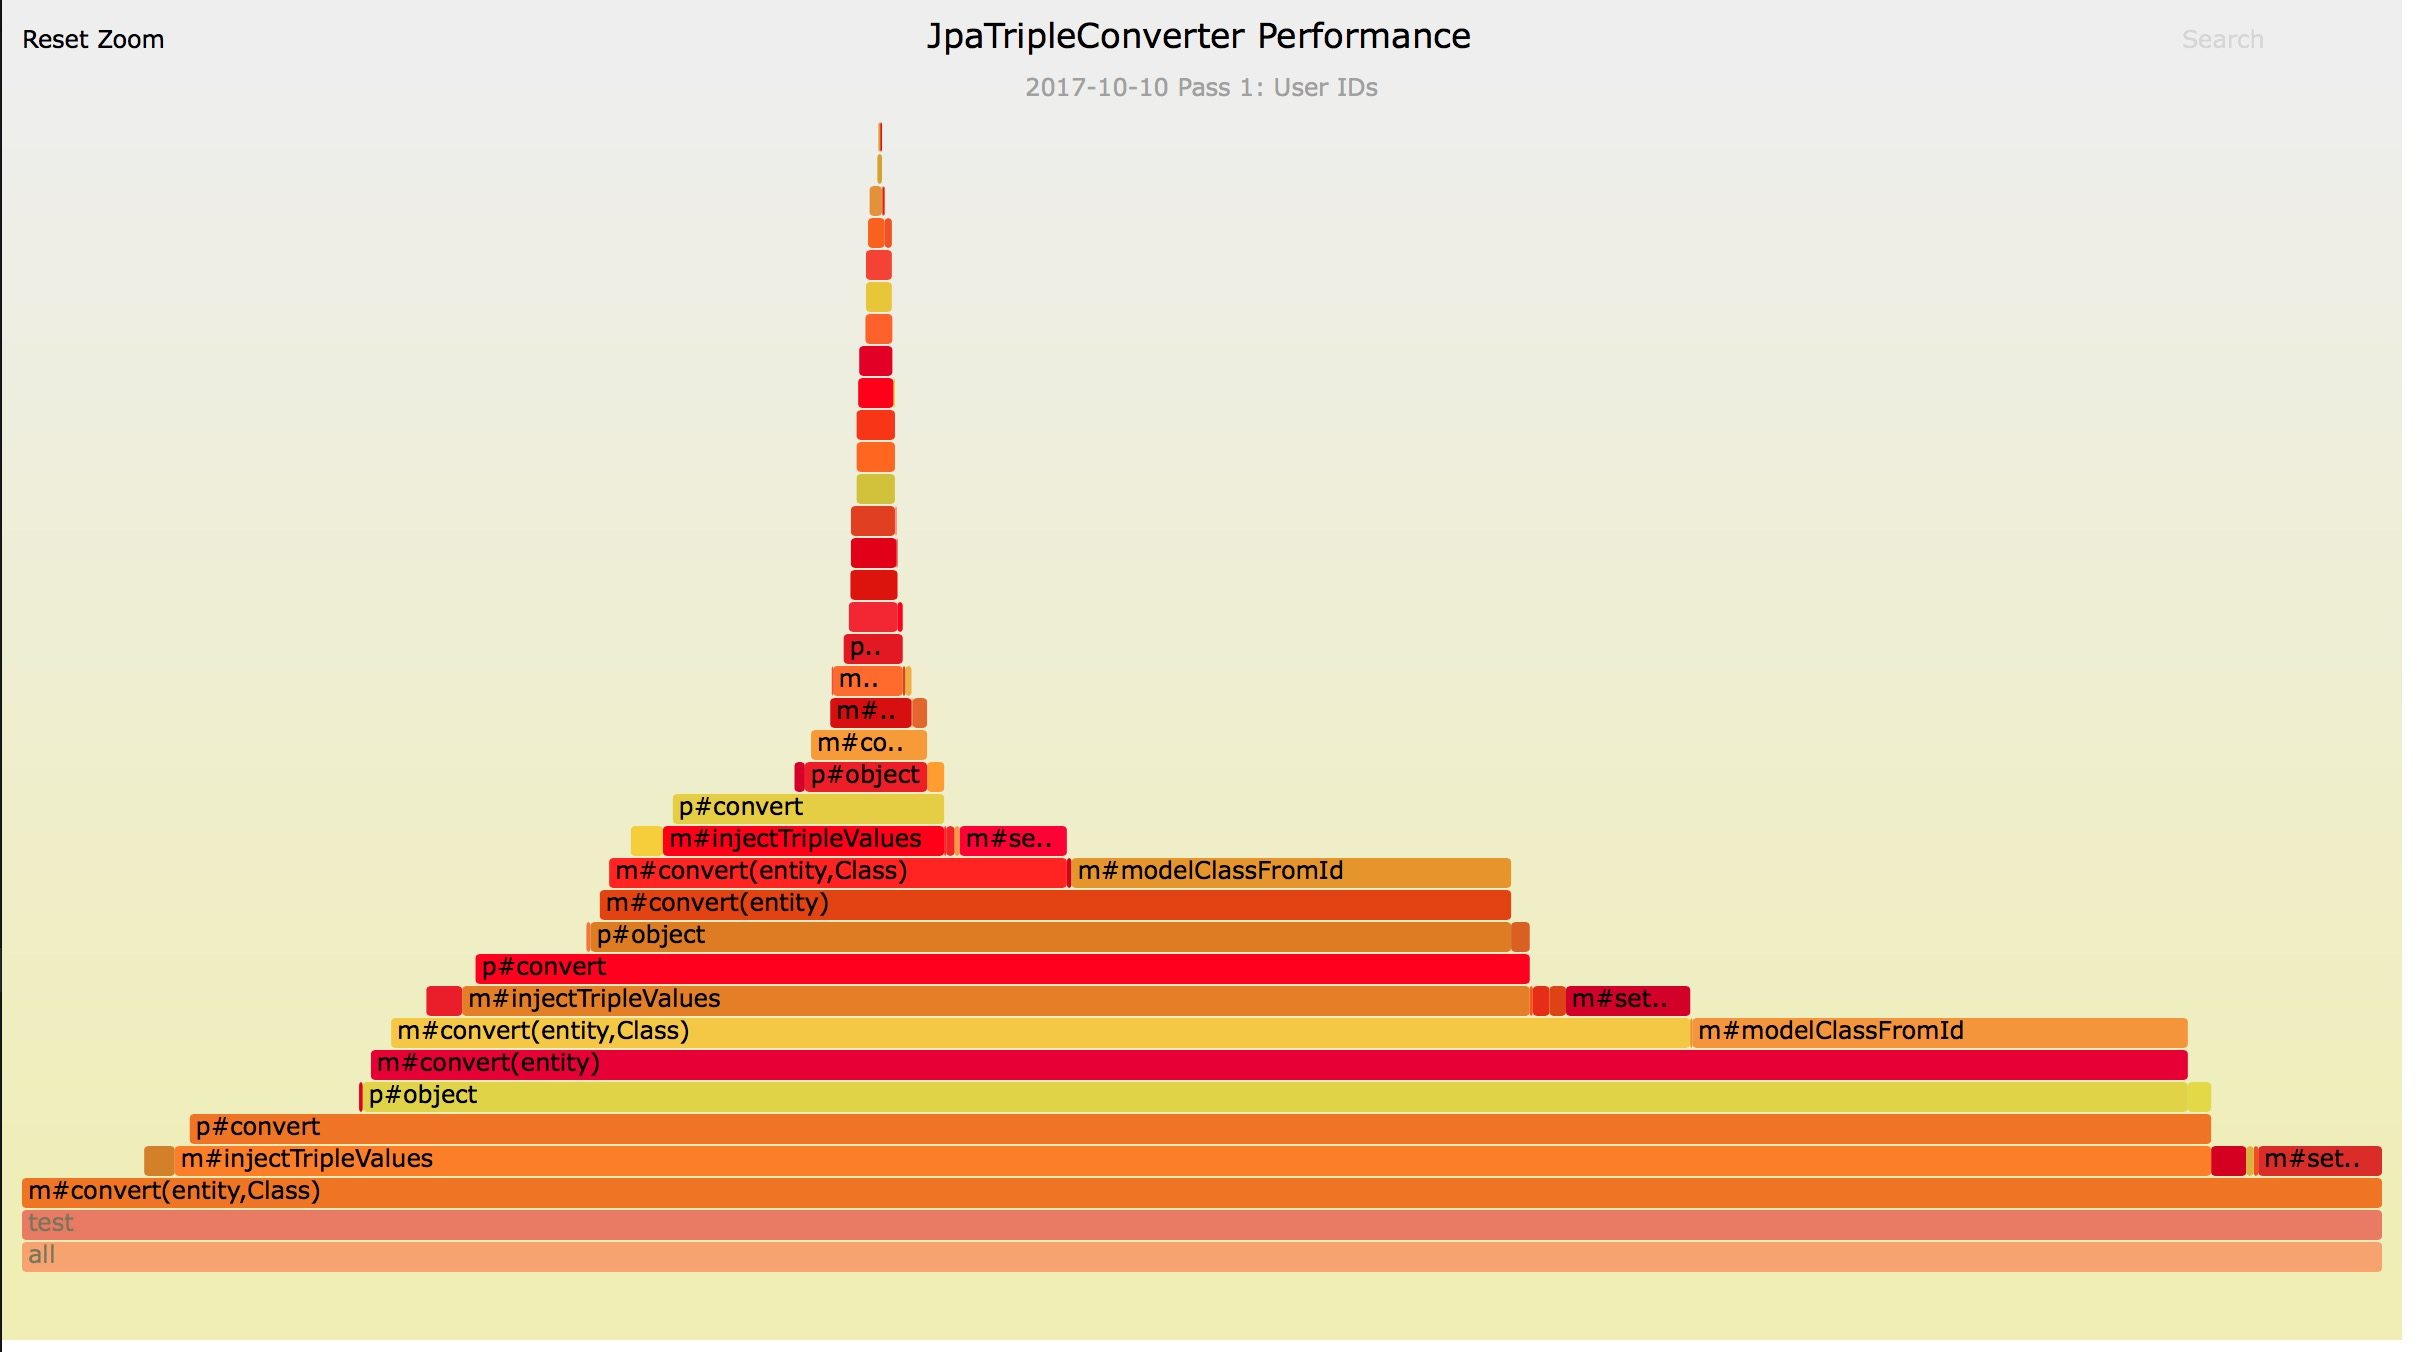
\includegraphics[width=\textwidth,keepaspectratio]{pictures/flame-graph-example.jpg}
		\end{center}
		\legend{Fonte: https://rickosborne.org/blog/tag/flame-graph/}
	\end{figure}
\end{description}

%\capepigrafe[0.5\textwidth]{``Frase espirituosa de um autor famoso''}{Autor famoso}

%\begin{citacaoLonga}
%	\blindtext
%\end{citacaoLonga}

%\blinddocument


% ========== Referências ==========
% --- IEEE ---
%	http://www.ctan.org/tex-archive/macros/latex/contrib/IEEEtran
%\bibliographystyle{IEEEbib}

% --- ABNT (requer ABNTeX 2) ---
%	http://www.ctan.org/tex-archive/macros/latex/contrib/abntex2
\bibliographystyle{abntex2-num}

\bibliography{referencias}


% ========== Apêndices (opcional) ==========
%\apendice
%\chapter{}
%\chapter{Beta}


% ========== Anexos (opcional) ==========
%\anexo
%\chapter{Alpha}
%\chapter{}



\end{document}
